\documentclass{article}

\usepackage{amsmath,geometry,amsfonts,array,makecell,enumitem,bm,esint,booktabs,multirow,mathtools,upgreek,amssymb,pgfplots, chemfig, tikzorbital,subcaption,adjustbox,svg}
\usepackage[amsmath]{ntheorem}
\usepackage[hidelinks,naturalnames]{hyperref}
\usepackage[nameinlink,noabbrev]{cleveref}
\usepackage{fancyhdr}
\pagestyle{fancy}
\fancyhead[L]{\itshape\nouppercase{\leftmark}}
\fancyhead[R]{M1 Inorganic Materials}

\title{Inorganic Materials}
\author{Yue Wu}

\geometry{a4paper,hmargin=1.1in,vmargin=1.2in}

\setlength{\parskip}{1em}
\tolerance=1000
\emergencystretch=1em
\hyphenpenalty=1000
\exhyphenpenalty=100
\righthyphenmin=3

\svgsetup{
  inkscapeexe="C:/Program Files/Inkscape/bin/inkscape.exe",
}

\pgfplotsset{compat=1.18}
\usetikzlibrary{decorations.markings}

\theoremstyle{plain}\theoremheaderfont{\normalfont\itshape}\theorembodyfont{\rmfamily}\theoremseparator{.}\newtheorem*{rem}{Remark}\newtheorem*{ex}{Example}\newtheorem*{proof}{Proof}\newtheorem*{altp}{Alternative proof}

\theoremstyle{plain}\theoremheaderfont{\normalfont\bfseries}\theorembodyfont{\rmfamily}\theoremseparator{.}\newtheorem{thm}{Theorem}[section]\newtheorem{lem}[thm]{Lemma}\newtheorem{prop}[thm]{Proposition}\newtheorem*{cor}{Corollary}\newtheorem{defn}[thm]{Definition}\newtheorem{clm}[thm]{Claim}\newtheorem{clminproof}{Claim}

\theoremstyle{break}\theoremheaderfont{\normalfont\itshape}\theorembodyfont{\rmfamily}\theoremseparator{.\medskip}\newtheorem*{proofskip}{Proof}\newtheorem*{exs}{Examples}\newtheorem*{rems}{Remarks}

\theoremstyle{break}\theoremheaderfont{\normalfont\bfseries}\theorembodyfont{\rmfamily}\theoremseparator{.\medskip}\newtheorem{lemskip}[thm]{Lemma}\newtheorem{defnskip}[thm]{Definition}\newtheorem{propskip}[thm]{Proposition}\newtheorem{thmskip}[thm]{Theorem}

\crefname{thm}{Theorem}{Theorems}\crefname{defn}{Definition}{Definitions}\crefname{lem}{Lemma}{Lemmas}\crefname{lemskip}{Lemma}{Lemmas}\crefname{cor}{Corollary}{Corollaries} \crefname{prop}{Proposition}{Propositions}\crefname{clm}{Claim}{Claims}

\setcounter{tocdepth}{2}
\setcounter{section}{0}
\numberwithin{equation}{section}

\newcommand{\qed}{\hfill\ensuremath{\Box}}
\newcommand{\unit}[1]{\ \mathrm{#1}}
\newcommand{\ii}{\mathrm{i}}
\newcommand{\ee}{\mathrm{e}}
\newcommand{\tp}{^\mathrm{T}}
\newcommand{\dd}[2][]{\mathrm{d}^{#1} #2\,}
\renewcommand{\d}[2][]{\mathrm{d}^{#1} #2}
\newcommand{\dv}[3][]{\frac{\mathrm{d}^{#1} #2}{{\mathrm{d} #3}^{#1}}}
\newcommand{\pdv}[3][]{\frac{\partial^{#1} #2}{{\partial #3}^{#1}}}
\newcommand{\bra}[1]{\left\langle #1 \right|}
\newcommand{\ket}[1]{\left| #1 \right\rangle}
\newcommand{\braket}[2]{\left\langle #1 \middle| #2 \right\rangle}
\newcommand{\mel}[3]{\left\langle #1 \middle| #2 \middle| #3 \right\rangle}
\newcommand{\eval}[1]{\left\langle #1 \right\rangle}
\newcommand{\expval}[2]{\left\langle #2 \middle| #1 \middle| #2 \right\rangle}
\newcommand{\vb}[1]{\bm{\mathrm{#1}}}
\newcommand{\vu}[1]{\hat{\bm{\mathrm{#1}}}}
\newcommand{\cross}{\bm{\times}}
\newcommand{\vdot}{\bm{\cdot}}
\newcommand{\abs}[1]{\left| #1 \right|}
\newcommand{\norm}[1]{\left\| #1 \right\|}
\newcommand{\grad}{\vb{\nabla}}
\renewcommand{\div}{\vb{\nabla}\cdot}
\newcommand{\curl}{\vb{\nabla}\times}
\newcommand{\laplacian}{\nabla^2}
\renewcommand{\Re}{\operatorname{Re}}
\renewcommand{\Im}{\operatorname{Im}}
\newcommand{\hb}{\mathcal{H}}
\newcommand{\NN}{\mathbb{N}}
\newcommand{\ZZ}{\mathbb{Z}}
\newcommand{\QQ}{\mathbb{Q}}
\newcommand{\RR}{\mathbb{R}}
\newcommand{\CC}{\mathbb{C}}
\newcommand{\nuc}{_{\text{n}}}
\newcommand{\el}{_{\text{e}}}

\usetikzlibrary{arrows.meta,calc, math}

\setchemfig{
  atom sep=2em,
  bond style={line width=0.8pt},
  cram width=2pt
}


\begin{document}
    \setlength{\parindent}{0pt}
	\Huge\textsf{\textbf{Inorganic Materials}}
		
	\Large\textsf{\textbf{University of Cambridge Part III Natural Sciences Tripos}}

	\noindent\makebox[\linewidth]{\rule{\textwidth}{2pt}}

	\large\textsf{\textbf{Yue Wu}}
	\begin{itemize}[topsep=0pt,leftmargin=15pt]
		\item[] \textit{Yusuf Hamied Department of Chemistry\\
		Lensfield Road,\\
		Cambridge, CB2 1EW}\\

		\textit{yw628@cam.ac.uk}
	\end{itemize}
    \thispagestyle{empty}
    \pagenumbering{roman}
    \setlength{\parindent}{15pt}

    \newpage
    \begin{center}
		\textbf{\Large{Acknowledgements}}
	\end{center}
	\large
	Nothing in these lecture notes is original. They are largely based on the notes by Prof. Paul Wood, who lectured this course in 2025. Moreover, they are nowhere near accurate representations of what was actually lectured, and in particular, all errors are almost surely mine.

    \vskip 30pt

    \begin{center}
		\textbf{\Large{Preface}}
	\end{center}
	\large
    This course focuses on the magnetic properties of inorganic materials. It is not a theoretical course, so it will be pretty handwavy on quantum mechanical/statistical mechanical arguments. But I, as a theoretical chemist though, have tried my best to make this course notes more rigorous than the original official notes without being too pedantic. 
    
	\normalsize
    \newpage
	\tableofcontents
	\newpage
    \pagenumbering{arabic}

    \section{Magnetism in a Single Ion}
    \subsection{Magnetic Moment}
    In the 1820's Oersted showed that an electric current \(\vb{J}\), caused by the movement of charge carriers like electrons, can generate a magnetic field given by\footnote{The full form of this equation is
    \begin{equation}
        \curl \vb{B}=\mu_0\left(\vb{J}+\epsilon_0\pdv{\vb{E}}{t}\right)\,,
    \end{equation}
    where the latter term is something known as a \textit{displacement current}. It comes when we're working with something like a capacitor, but we are not dealing with them in this course. Moreover, we are not distinguishing \(\vb{H}\) and \(\vb{B}\) and calling both of them `magnetic field' for some reason that will be explained later.
    }
    \begin{equation}
        \curl \vb{B}=\mu_0\vb{J}\,,
    \end{equation}
    where \(\mu_0\) is the permeability of free space. On the other hand, it is also found that a rotational current \(I\) in a circular wire generates something called a \textit{magnetic moment}, \(\vb{\mu}\) (or sometimes \(\vb{m}\)), given by
    \begin{equation}
        \vb{\mu}=I\vu{n}A\,,
    \end{equation}
    where \(A\) is the area enclosed by the circular wire and \(\vu{n}\) is the unit normal, such that placing the magnetic moment \(\vb{\mu}\) in a magnetic field \(\vb{B}\) will experience a torque
    \begin{equation}
        \vb{\tau}=\vb{\mu}\cross\vb{B}\,.
    \end{equation}
    This will lead to an additional potential energy
    \begin{equation}
        E=-\vb{\mu}\vdot\vb{B}
    \end{equation}
    for a magnetic moment placed in a magnetic field which favours the magnetic moment to align with the magnetic field, just like an electric dipole moment will align with an electric field.

    \begin{figure}[ht!]
        \centering
        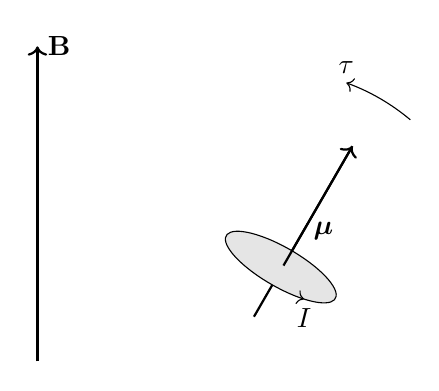
\begin{tikzpicture}
            \draw[->,thick] (240:0.5)--node[right]{\(\vb{\mu}\)}(60:2);
            \draw[->, rotate=-30, fill=gray!20] (0.38,0) arc [start angle=-60, end angle=305, x radius=0.8cm, y radius=0.25cm] node[below]{\(I\)};
            \draw[thick] (60:0.25)--(60:2);

            \draw[->,thick] (-3,-1)--(-3,3)node[right]{\(\vb{B}\)};
            \draw[->] (50:2.7) arc (50:70:2.7) node[above]{\(\tau\)};
        \end{tikzpicture}
        \caption{A charged particle with angular momentum will experience a torque in a magnetic field.}
    \end{figure}

    This reveals the close link between the angular momentum of a moving current and the magnetic moment. Suppose a particle of charge \(+q\) of mass \(m\) is rotating around a circle of radius \(r\) with angular velocity \(\vb{\omega}\). This is effectively a current
    \begin{equation}
        I=\frac{Q}{t}=\frac{\omega q}{2\pi}\,,
    \end{equation}
    which produces a magnetic moment
    \begin{equation}
        \vb{\mu} =\frac{\vb{\omega} q r^2}{2}\,.
    \end{equation}
    Since the particle carries an angular momentum
    \begin{equation}
        \vb{L}=mr^2\vb{\omega}\,,
    \end{equation}
    we can conclude that the magnetic moment it creates is proportional to the angular momentum
    \begin{equation}
        \vb{\mu}=\gamma\vb{L}=\frac{q}{2m}\vb{L}\,,
    \end{equation}
    where the proportionality constant \(\gamma\) is known as the \textit{gyromagnetic ratio}. This magnetic moment, coming from orbital angular momentum (momentum caused by particle orbiting around some point), is often written with a seemingly redundant extra factor
    \begin{equation}
        \vb{\mu}_{L}=g_L \frac{q}{2m}\vb{L}\,,
    \end{equation}
    where \(g_L=1\) is the Land\'{e} \(g\)-factor for orbital angular momentum for a reason that will be apparent immediately.

    Some charge-carrying particles, like electrons, have another natural source of angular momentum --- that is its spin. For a particle of spin \(S\), it carries a spin angular momentum of magnitude
    \begin{equation}
        \norm{\vb{S}}=\hbar\sqrt{S(S+1)}\,,
    \end{equation}
    which also leads to a magnetic moment
    \begin{equation}
        \vb{\mu}_S = \gamma \vb{S}=g_S \frac{q}{2m}\vb{S}\,.
    \end{equation}
    The spin of a particle does not come from its circular motion. It is intrinsic to the particle so we have no reason to assume \(g_S=1\) as for the orbital angular momentum case. For free electrons, \(g_{S, e-}\approx 2.0\),\footnote{In Dirac's theory, every point-like Fermion should have \(g_S=2\) exactly, while it is actually slightly above \(2\) for some subtle Quantum Field Theory effects. This is known as the anomalous magnetic moment.} while for other particles like a proton, it takes some other values that are not relevant for us. For a single, isolated free electron, the magnitude of the magnetic moment is
    \begin{equation}
        \mu_S=g_S\mu_{\text{B}}\sqrt{S(S+1)}\,,
    \end{equation}
    where \(S=\frac{1}{2}\), and \(\mu_{\text{B}}=e\hbar/2m_e\) is the Bohr's magneton (also denoted \(\beta\)) which characterises the strength of the magnetic moment of an electron. Note that since the charge of an electron is negative, \(q=-e\), its magnetic moment \(\vb{\mu}_S\) is in the opposite direction of its spin \(\vb{S}\), i.e. the gyromagnetic ratio is negative. We will take extra care on whether we are talking about the direction of the spin or the direction of the magnetic moment in future.

    \subsection{Magnetic Moment of Ions and Atoms}
    In an ion or atom, there are two main sources of angular momenta --- the spins and the orbital angular momentum of the electrons. The nucleus also carries nuclear spin, but the magnetic moment is proportional to \(m^{-1}\), and since nuclei are much heavier than the electrons, we are ignoring the nuclear contribution.

    The Schr\"{o}dinger equation tells us that the electronic spins and orbital angular momentum of an atom (ion) are characterised by two quantum numbers, the total spin quantum number \(S\) and the total orbital angular momentum quantum number \(L\). However, due to relativistic effects that are neglected in Schr\"{o}dinger's equation, the spin and orbital angular momentum can interact, and the effect is that these two numbers are no longer well defined. This process is called \textit{spin-orbit coupling}, and the overall result is that the spin is well-described by the total angular momentum quantum number \(J\).

    The strength of spin-orbit coupling is characterised by the spin-orbit coupling constant \(\lambda\), and the magnitude of \(\lambda\) is strongly dependent on the nuclear charge, \(\lambda\propto Z^4\). This means that for atoms not too heavy (up to around the third row transition metals), we can treat the spin-orbit coupling as a perturbation and still sensibly talk about the \(L\) and \(S\) values of an electronic term, and the possible \(J\) values are \(J=L+S, \dots, \abs{L-S}\). This is the \textit{\(LS\) coupling} (or \textit{Russell--Saunders coupling}) scheme. For the remainder of this course, we will always assume that the spin-orbit coupling is weak enough that the \(LS\) coupling scheme always applies.
    
    The way to work out the \(L\), \(S\) and \(J\) values for an electronic configuration should be familiar from Part IB and Part II, and the ground term (level) is determined by the Hund's rules.

    \begin{ex}
        \textit{Gaseous \(\mathrm{Ti^{3+}}\) ion.}

        A free \(\mathrm{Ti^{3+}}\) ion has electron configuration \(\mathrm{[Ar]\ 3d^1}\). The \(L\) and \(S\) values satisfying the Hund's first and second rules can be worked out using the box method.

        \begin{figure}[ht!]
            \centering
            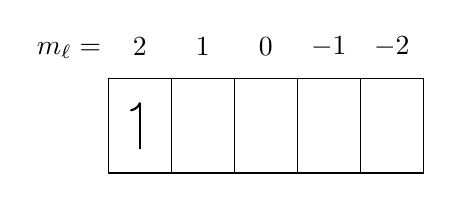
\begin{tikzpicture}
                \foreach \i in {-2,...,2}{
                    \draw (0.8*\i-0.4,-0.6) rectangle (0.8*\i + 0.4, 0.6);
                    \node at (-0.8*\i,1) {\(\i\)};
                }
                \draw[arrows = {->[left]}, thick] (-1.6,-0.3)--(-1.6,0.3);
                \node at (-2.5,0.95){\(m_\ell = \)};
            \end{tikzpicture}
        \end{figure}

        This gives \(L=2\) and \(S=\frac{1}{2}\), with spin multiplicity \(2S+1=2\). The available \(J\) values are \(J=\frac{5}{2}, \frac{3}{2}\). This is less than half-filled, so we need to minimise \(J\), giving \(J=\frac{3}{2}\). The ground level is therefore \(^2 D_{\frac{3}{2}}\).

        \begin{figure}[ht!]
            \centering
            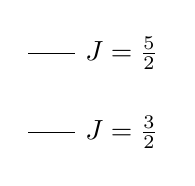
\begin{tikzpicture}
                \draw (-0.3,0)--(0.3,0)node[right]{\(J=\frac{3}{2}\)};
                \draw (-0.3,1)--(0.3,1)node[right]{\(J=\frac{5}{2}\)};
            \end{tikzpicture}
        \end{figure}
    \end{ex}
    
    \subsubsection{Free Ions}
    When both the electronic spin and angular momentum are present in a free ion (atom), the overall magnetic moment is proportional to the total angular momentum:
    \begin{equation}\label{free_ion_m_J}
        \mu_J = g_J\mu_{\text{B}}\sqrt{J(J+1)}\,,
    \end{equation}
    where the Land\'{e} \(g\)-factor for the total angular momentum is given by the complicated formula
    \begin{equation}
        g_{J}=g_{L}\frac{J(J+1)-S(S+1)+L(L+1)}{2J(J+1)}+g_{S}\frac{J(J+1)+S(S+1)-L(L+1)}{2J(J+1)}\,.
    \end{equation}
    We have \(g_L=1\), and if we take \(g_S=2\), the above equation simplifies to
    \begin{equation}\label{free_ion_g_J}
        g_{J}\approx 1 + \frac{J(J+1)+S(S+1)-L(L+1)}{2J(J+1)}\,.
    \end{equation}

    \subsubsection{Transition Metal Complexes}
    Free atoms and ions are of little interest to chemists. Instead, the materials showing the most interesting magnetic properties are the transition metal complexes, which will be the main topic of this course.

    The above equation cannot be directly applied to transition metal complexes, because we need a bit extra considerations on the orbital angular momentum.

    We now make the claim that for an ion to carry orbital angular momentum, it must have a set of partially filled degenerate orbitals. This can be seen from the atomic orbitals: an orbital with angular momentum quantum number \(\ell\) is \((2\ell+1)\)-degenerate, and the non-degenerate \(\mathrm{s}\)-orbital carries zero orbital angular momentum. The reason is that if several orbitals are degenerate, then any complex linear combination of them is also an allowed stationary state. The electron can occupy a coherent superposition with relative phases which evolve in a way such that it produces a probability density that circulates around the nucleus, leading to orbital angular momentum --- this can be imagined by electrons hopping between degenerate orbitals at different orientations.

    However, the degeneracies of the valence \(\mathrm{d}\) orbitals are broken in transition metal complexes due to ligand field splitting. This leads to the quenching of the orbital angular momentum. For example, in an octahedral complex, the \(\mathrm{d}\) orbitals are split into a \(T_{2g}\) set and a \(E_g\) set. The \(E_g\) set is only doubly degenerate, and since the orbital angular momentum quantum number can only be integers, it can carry no momentum. The \(T_{2g}\) set, on the other hand, are triply degenerate, and can carry one unit of angular momentum. Hence, if an octahedral complex has term symbol \(A\) or \(E\), it effectively has \(L_{\text{eff}}=0\), and we say that the angular momentum is completely quenched, while a complex with term symbol \(T\) is partially quenched, and has \(L_{\text{eff}}=1\).

    \begin{ex}
        \textit{Ground state term symbols and orbital angular momentum of octahedral complexes.}
        \begin{figure}[ht!]
            \centering
            \begin{tikzpicture}
                \draw (-1.6,0)--(-0.8,0);
                \draw (-0.4,0)--(0.4,0);
                \draw (0.8,0)--(1.6,0);
                \draw (-1,1.3)--(-0.2,1.3);
                \draw (0.2,1.3)--(1,1.3);
                \node at (-2.3,0) {\(t_{2g}\)};
                \node at (-2.3,1.3) {\(e_{g}\)};
                \foreach \i in {-1,0,1}{
                    \draw[arrows = {->[left]},thick] (1.2*\i-0.06,-0.2)--(1.2*\i-0.06,0.4);
                }
                \foreach \i in {-1,0}{
                    \draw[arrows = {->[left]},thick] (1.2*\i+0.06,0.4)--(1.2*\i+0.06,-0.2);
                }
                \foreach \i in {-1,0}{
                    \draw[arrows = {->[left]},thick] (1.2*\i+0.6-0.06,1.1)--(1.2*\i+0.6-0.06,1.7);
                }

                \node at (0,-1) {\(\mathrm{Co^{2+}}\), \(d^7\) HS};
                \node at (0,-1.55) {\(T\)};
                \node at (0,-2.1) {\(L_{\text{eff}}=1\).};

                \begin{scope}[shift={(5,0)}]
                    \draw (-1.6,0)--(-0.8,0);
                    \draw (-0.4,0)--(0.4,0);
                    \draw (0.8,0)--(1.6,0);
                    \draw (-1,1.3)--(-0.2,1.3);
                    \draw (0.2,1.3)--(1,1.3);
                    \foreach \i in {-1,0,1}{
                        \draw[arrows = {->[left]},thick] (1.2*\i-0.06,-0.2)--(1.2*\i-0.06,0.4);
                    }
                    \foreach \i in {-1}{
                        \draw[arrows = {->[left]},thick] (1.2*\i+0.6-0.06,1.1)--(1.2*\i+0.6-0.06,1.7);
                    }
                    \node at (0,-1) {\(\mathrm{Cr^{2+}}\), \(d^4\) HS};
                    \node at (0,-1.55) {\(E\)};
                    \node at (0,-2.1) {\(L_{\text{eff}}=0\).};
                \end{scope}

                \begin{scope}[shift={(10,0)}]
                    \draw (-1.6,0)--(-0.8,0);
                    \draw (-0.4,0)--(0.4,0);
                    \draw (0.8,0)--(1.6,0);
                    \draw (-1,1.3)--(-0.2,1.3);
                    \draw (0.2,1.3)--(1,1.3);
                    \foreach \i in {-1,0,1}{
                        \draw[arrows = {->[left]},thick] (1.2*\i-0.06,-0.2)--(1.2*\i-0.06,0.4);
                    }
                    \foreach \i in {-1,0}{
                        \draw[arrows = {->[left]},thick] (1.2*\i+0.6-0.06,1.1)--(1.2*\i+0.6-0.06,1.7);
                    }
                    \node at (0,-1) {\(\mathrm{Mn^{2+}}\), \(d^5\) HS};
                    \node at (0,-1.55) {\(A\)};
                    \node at (0,-2.1) {\(L_{\text{eff}}=0\).};
                \end{scope}
                
            \end{tikzpicture}
        \end{figure}
    \end{ex}

    To avoid this complication, it is often good enough to only consider the contribution of the electron spins to the magnetic moment. This leads to the spin only formula
    \begin{equation}
        \mu_{\text{so}}=g_{\text{so}}\mu_{\text{B}}\sqrt{S(S+1)}
    \end{equation}
    for an ion of spin quantum number \(S\). This is the formula you have seen throughout in Part IB and Part II when calculating the effective magnetic moment of e.g. a transition metal complex ion.

    If we are making a very crude estimation, then we can directly take the Land\'{e} \(g\)-factor to be that of a free electron, \(g_{\text{so}}\approx g_{S, e^-}\approx 2.0\). However, due to the fact that the electron is not completely free in the complexes and that we have ignored the orbital angular momentum contribution, we usually need a slightly larger value of \(g_{\text{so}}\) to match the experimental value of measured magnetic moment.
    \begin{ex}
        \textit{\(\mathrm{Ti^{3+}}\) complex: \(\mathrm{[Ti(CN)_6]^{3-}}\)}

        Let's return to the \(\mathrm{Ti^{3+}}\) example, but this time in a complex \(\mathrm{[Ti(CN)_6]^{3-}}\). Suppose this complex is octahedral, then the orbital diagram is shown below.

        \begin{figure}[ht!]
            \centering
            \begin{tikzpicture}
                \draw (-1.6,0)--(-0.8,0);
                \draw (-0.4,0)--(0.4,0);
                \draw (0.8,0)--(1.6,0);
                \draw (-1,1.7)--(-0.2,1.7);
                \draw (0.2,1.7)--(1,1.7);
                \node at (-2.3,0) {\(t_{2g}\)};
                \node at (-2.3,1.7) {\(e_{g}\)};
                \draw[arrows = {->[left]},thick] (-1.2,-0.2)--(-1.2,0.4);
                \node at (0,-1) {octahedral};

                \draw[dashed] (1,1.7)--(5,2);
                \draw[dashed] (1,1.7)--(5,1.3);
                \draw (5,2)--(5.8,2);
                \draw (5,1.3)--(5.8,1.3);
                \draw[dashed] (1,0)--(4.4,0.2);
                \draw[dashed] (1,0)--(5,-0.4);
                \draw (5,-0.4)--(5.8,-0.4);
                \draw (4.4,0.2)--(5.2,0.2);
                \draw (5.6,0.2)--(6.4,0.2);
                \draw[arrows = {->[left]},thick] (5.4,-0.6)--(5.4,0);
                \node at (5.4,-1) {distorted};
            \end{tikzpicture}
        \end{figure}

        The term symbol is \(^2 T_{2g}\), with \(L=1\) and \(S=\frac{1}{2}\). The available \(J\) values are \(\frac{1}{2}\) and \(\frac{3}{2}\).

        However, this complex has asymmetrically filled \(t_{2g}\) level, and so it is susceptible to Jahn--Teller distortion. This further breaks the degeneracy of the \(t_{2g}\) level and leads to a complete quenching of angular momentum.
    \end{ex}

    Due to the double effect of ligand field splitting and Jahn--Teller distortion, the orbital angular momentum of transition metal complexes are almost always completely quenched, and so it is fine to consider \(S\) only.

    \subsubsection{Lanthanide Ions}
    The special case comes to the lanthanide \(3^{+}\) ions. We have learned in Part II A1 that those ions have extremely contracted \(\mathrm{4f}\) orbitals, and the interactions between the metal ions and ligands are predominantly ionic with little covalency. As a result, the degeneracy of the \(\mathrm{4f}\) orbitals are not broken and they behave closely to free ions. Therefore, the formula of the magnetic moments and Land\'{e} \(g\)-factors for free ions, (\ref{free_ion_m_J}) and (\ref{free_ion_g_J}), work extremely well for lanthanide ions.

    \subsubsection{Spin Crossover Complex}
    We are familiar with the idea that a coordination complex can be classified as being either high or low spin. However, there are possibilities that the difference in crystal field stabilisation energies between the two spin states are so small that it is comparable to the thermal energy at some achievable temperature.
    
    The most common combination of metal and ligand that gives rise to this situation is \(\mathrm{Fe\ (II)}\) with moderately strong \(\sigma\)-donor ligands (e.g. \(\mathrm{S}\) or \(\mathrm{N}\)-donors). In these materials the low spin state (with \(S=0\)) is always lower in energy (enthalpy) than the high spin state (with \(S=2\)). However, a spin state \(S\) has degeneracy \(2S+1\), leading to an associated molar entropy
    \begin{equation}
        S_S=R\ln(2S+1)\,,
    \end{equation}
    where we have assumed the orbital angular momentum to be completely quenched. For free ions or lanthanide complexes where the orbital angular momentum is significant, the corresponding entropy is
    \begin{equation}
        S_J=R\ln(2J+1)\,.
    \end{equation}
    As the temperature is raised the population of the energetically excited state increases (from zero) and the sample switches from being diamagnetic to paramagnetic.

    For example, consider the octahedral \(\mathrm{Fe\ (II)}\) complex shown in \cref{Fig:crossover_structure} and the plot of \(\mu^2\) (or equivalently \(\chi T\), see later) against temperature is shown in \cref{Fig:crossover_plot}. The molecular orbital diagrams of the low spin and high spin states are shown below.

    \begin{figure}[ht!]
        \centering
        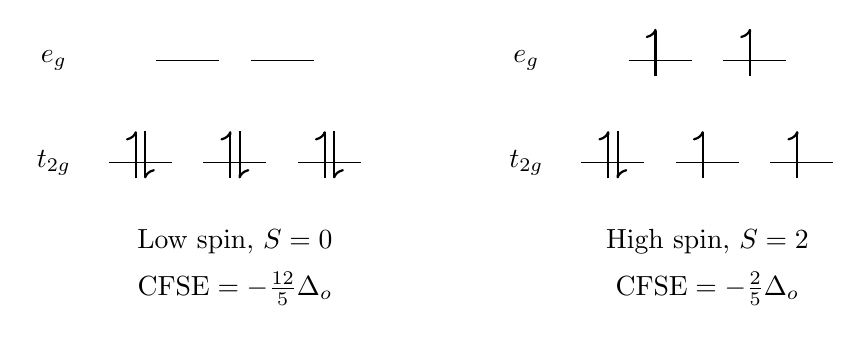
\begin{tikzpicture}
            \draw (-1.6,0)--(-0.8,0);
            \draw (-0.4,0)--(0.4,0);
            \draw (0.8,0)--(1.6,0);
            \draw (-1,1.3)--(-0.2,1.3);
            \draw (0.2,1.3)--(1,1.3);
            \node at (-2.3,0) {\(t_{2g}\)};
            \node at (-2.3,1.3) {\(e_{g}\)};
            \foreach \i in {-1,0,1}{
                \draw[arrows = {->[left]},thick] (1.2*\i-0.06,-0.2)--(1.2*\i-0.06,0.4);
            }
            \foreach \i in {-1,0,1}{
                \draw[arrows = {->[left]},thick] (1.2*\i+0.06,0.4)--(1.2*\i+0.06,-0.2);
            }

            \node at (0,-1) {Low spin, \(S=0\)};
            \node at (0,-1.6) {\(\mathrm{CFSE}=-\frac{12}{5}\Delta_o\)};

            \begin{scope}[shift={(6,0)}]
                \draw (-1.6,0)--(-0.8,0);
                \draw (-0.4,0)--(0.4,0);
                \draw (0.8,0)--(1.6,0);
                \draw (-1,1.3)--(-0.2,1.3);
                \draw (0.2,1.3)--(1,1.3);
                \node at (-2.3,0) {\(t_{2g}\)};
                \node at (-2.3,1.3) {\(e_{g}\)};
                \foreach \i in {-1,0,1}{
                    \draw[arrows = {->[left]},thick] (1.2*\i-0.06,-0.2)--(1.2*\i-0.06,0.4);
                }
                \foreach \i in {-1}{
                    \draw[arrows = {->[left]},thick] (1.2*\i+0.06,0.4)--(1.2*\i+0.06,-0.2);
                }
                \foreach \i in {-1,0}{
                    \draw[arrows = {->[left]},thick] (1.2*\i+0.6-0.06,1.1)--(1.2*\i+0.6-0.06,1.7);
                }

                \node at (0,-1) {High spin, \(S=2\)};
                \node at (0,-1.6) {\(\mathrm{CFSE}=-\frac{2}{5}\Delta_o\)};
            \end{scope}
        \end{tikzpicture}
    \end{figure}

    \begin{figure}[ht!]
        \centering
        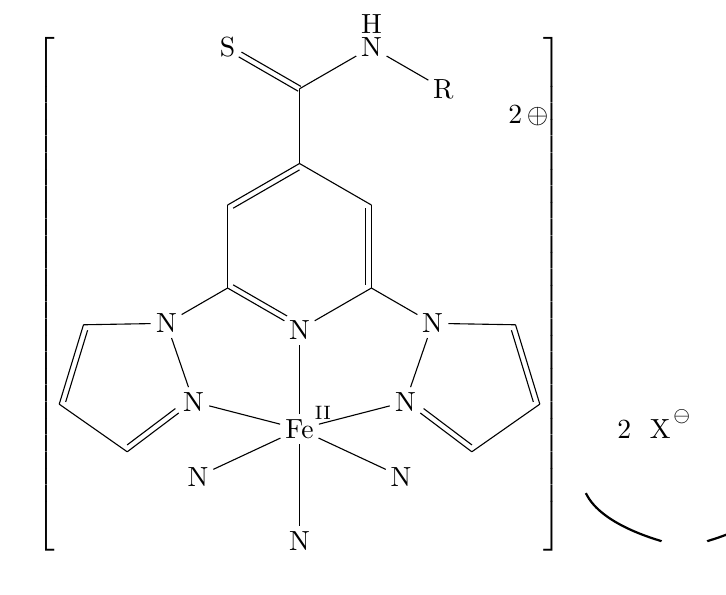
\begin{tikzpicture}
            \node at (0,0){
                \chemleft[\chemfig{
                    \charge{35:2.3pt=\scriptsize\(\mathrm{II}\)}{Fe}?[a]?[b]
                    (-[:90,1.2]  N*6(-[:60](-[,0.85]N*5([:-55]-N?[a]=-=-))=-(-[,0.9](=[:150]S)-[:30]\chemabove{N}{H}-[:-30]R)=-(-[,0.85]N*5([:-125]-=-=N?[b]-))=))
                    (-[:-90,1.35]@{c}N)
                    (-[:-155,1.35]@{d}N)
                    (-[:-25,1.35]@{e}N)
                }\chemright]\qquad 2 \ \chemfig{\charge{30:3pt=\scriptsize\(\ominus\)}{X}}
                \chemmove{\draw[-,thick,shorten <=1mm,shorten >=1mm](c)..controls +(180:2mm) and +(-65:7mm)..(d);}
                \chemmove{\draw[-,thick,shorten <=1mm,shorten >=1mm](c)..controls +(0:2mm) and +(-115:7mm)..(e);}
            };
            \node at (2.1,2.3) {\(2\,\oplus\)};
        \end{tikzpicture}
        \caption{The structure of a spin crossover complex, where \(\mathrm{R}\) is \(\mathrm{Me}\) or \(\mathrm{H}\) and \(\mathrm{X^-}\) is \(\mathrm{BF_4^-}\) or \(\mathrm{ClO_4^-}\).}
        \label{Fig:crossover_structure}
    \end{figure}

    \begin{figure}
        \centering
        % This file was created with matplot2tikz v0.4.0.
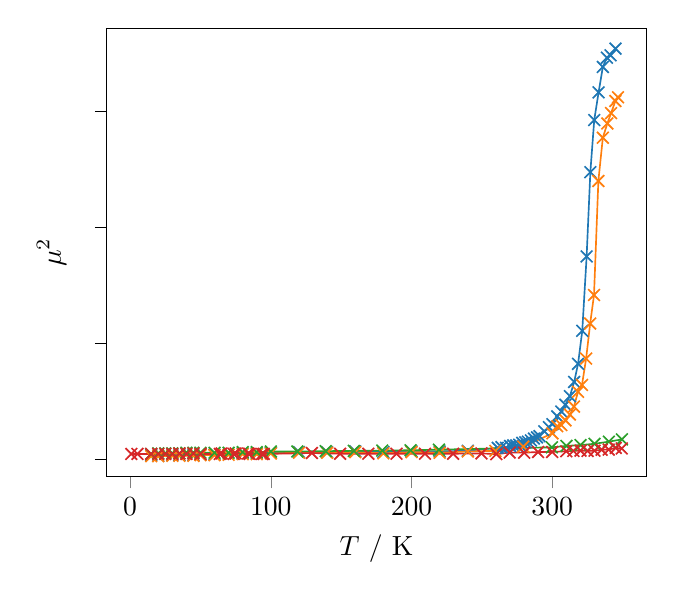
\begin{tikzpicture}

\definecolor{crimson2143940}{RGB}{214,39,40}
\definecolor{darkgray176}{RGB}{176,176,176}
\definecolor{darkorange25512714}{RGB}{255,127,14}
\definecolor{forestgreen4416044}{RGB}{44,160,44}
\definecolor{steelblue31119180}{RGB}{31,119,180}

\begin{axis}[
tick align=outside,
tick pos=left,
x grid style={darkgray176},
xlabel={\(\displaystyle T\) / \(\displaystyle \mathrm{K}\)},
xmin=-16.5854903156202, xmax=366.934851215292,
y grid style={darkgray176},
ylabel={\(\displaystyle \mu^2\)},
ymin=-3.04606060606061, ymax=74.2339393939394,
ytick style={color=black},
yticklabel=\empty,
]
\addplot [draw=steelblue31119180, fill=steelblue31119180, mark=x, only marks]
table{%
x  y
15 0.636363636363636
20 0.53030303030303
30 0.636363636363636
35 0.636363636363636
45 0.636363636363636
50 0.742424242424242
60 0.742424242424242
80 0.933333333333333
90 0.933333333333333
100 1.05
120 1.16666666666667
140 1.16666666666667
160 1.28333333333333
180 1.16666666666667
200 1.28333333333333
220 1.28333333333333
240 1.4
261.239711934156 1.90909090909091
263.940329218107 2.01515151515152
267.181069958848 1.90909090909091
270.061728395062 2.22727272727273
272.222222222222 2.33333333333333
274.382716049383 2.33333333333333
276.543209876543 2.43939393939394
278.703703703704 2.75757575757576
280.864197530864 2.86363636363636
282.664609053498 2.96969696969697
284.825102880658 3.18181818181818
286.985596707819 3.5
289.146090534979 3.71212121212121
290.946502057613 3.92424242424243
294.354569821328 4.76380344003295
297.6080247 5.46212121212121
300.128600823045 5.99242424242424
303.549382716049 7.31818181818182
306.430041152263 8.16666666666667
309.310699588477 9.33333333333333
312.551440329218 10.8181818181818
315.587306655314 13.2603187042842
318.343278463649 16.3831313131313
321.331447187929 22.0747474747475
324.434156378601 34.8939393939394
327.07475994513 49.4242424242424
329.839309367914 58.4075269085471
332.935913123656 63.1757982706972
335.956790123457 67.5606060606061
338.837448559671 69.1515151515152
341.442657877611 69.5590382257885
344.958847736626 70.7212121212121
};
\addplot [draw=darkorange25512714, fill=darkorange25512714, mark=x, only marks]
table{%
x  y
15 0.466666666666667
20 0.466666666666667
30 0.525
35 0.525
45 0.525
50 0.641666666666667
60 0.641666666666667
70 0.7
80 0.816666666666667
90 0.816666666666667
100 0.933333333333333
120 1.06060606060606
140 1.06060606060606
160 1.16666666666667
180 0.954545454545455
200 1.16666666666667
220 1.06060606060606
240 1.27272727272727
259.6193416 1.37878787878788
279.423868312757 2.12121212121212
300.128600823045 4.40151515151515
303.549382716049 5.62121212121212
306.430041152263 5.83333333333333
309.41081421494 6.64549161338152
312.551440329218 7.63636363636364
315.432098765432 9.01515151515151
318.312757201646 11.5606060606061
321.143935729133 12.7428829356366
324.074074074074 17.2878787878788
326.954732510288 23.3333333333333
329.682355967078 28.2479166666667
332.772232437323 47.9036643026005
335.956790123457 55.3636363636364
339.155082137241 57.8155333826066
341.806412894376 59.5979797979798
344.862090926906 61.6875901875902
346.73225308642 62.332702020202
};
\addplot [draw=forestgreen4416044, fill=forestgreen4416044, mark=x, only marks]
table{%
x  y
15 0.848484848484849
20 0.954545454545455
25 0.954545454545455
30 0.954545454545455
35 0.954545454545455
40 1.06060606060606
45 1.06060606060606
50 1.06060606060606
60 1.06060606060606
70 1.06060606060606
80 1.16666666666667
90 1.16666666666667
100 1.27272727272727
118.827160493827 1.27272727272727
138.991769547325 1.33113746157225
158.97633744856 1.37878787878788
179.16875773696 1.43483616654348
199.305555555556 1.48484848484848
219.470164609054 1.59090909090909
299.732510288066 1.98981481481482
310.081108240023 2.23467230443974
320.121170553269 2.38047138047138
330.055133481059 2.5998445998446
340.235907742368 2.96723044397463
349.502108418432 3.36120463898243
};
\addplot [draw=crimson2143940, fill=crimson2143940, mark=x, only marks]
table{%
x  y
0.847252481239409 0.848484848484849
5.22119341563786 0.848484848484849
15 0.848484848484849
20 0.848484848484849
25 0.848484848484849
30 0.848484848484849
35 0.932047750229577
40 0.848484848484849
45 0.932047750229577
50 0.848484848484849
63.7345679012346 0.848484848484849
65 0.932047750229577
73.649106808829 0.848484848484849
75 0.932047750229577
83.8991769547325 0.932047750229577
85 0.848484848484849
93.7789351851852 0.848484848484849
95 0.848484848484849
129.162379972565 1.00631313131313
149.258506473954 0.885802469135814
169.291636407649 0.885802469135814
189.316956657762 0.885802469135814
209.552725352002 0.885802469135814
229.552469135802 0.885802469135814
249.687738149672 0.940845959595966
260.262507441054 0.817800647989333
269.765275092138 1.08999634903249
280.033238366572 1.06831131831133
289.91224696486 1.18021334843766
299.948559670782 1.18916437098256
309.987891412217 1.31506422247163
315.001143118427 1.36902356902358
320.052509698069 1.42060388834583
325.117645938119 1.36798540965208
330.024744572158 1.41017938000697
335.078189300412 1.57676767676768
340.124229167439 1.60014560014561
345.124131417392 1.89605067064083
349.370967332216 1.79517396184063
};
\addplot [semithick, steelblue31119180, mark=x, mark size=3, mark options={solid}]
table {%
15 0.636363636363636
20 0.53030303030303
30 0.636363636363636
35 0.636363636363636
45 0.636363636363636
50 0.742424242424242
60 0.742424242424242
80 0.933333333333333
90 0.933333333333333
100 1.05
120 1.16666666666667
140 1.16666666666667
160 1.28333333333333
180 1.16666666666667
200 1.28333333333333
220 1.28333333333333
240 1.4
261.239711934156 1.90909090909091
263.940329218107 2.01515151515152
267.181069958848 1.90909090909091
270.061728395062 2.22727272727273
272.222222222222 2.33333333333333
274.382716049383 2.33333333333333
276.543209876543 2.43939393939394
278.703703703704 2.75757575757576
280.864197530864 2.86363636363636
282.664609053498 2.96969696969697
284.825102880658 3.18181818181818
286.985596707819 3.5
289.146090534979 3.71212121212121
290.946502057613 3.92424242424243
294.354569821328 4.76380344003295
297.6080247 5.46212121212121
300.128600823045 5.99242424242424
303.549382716049 7.31818181818182
306.430041152263 8.16666666666667
309.310699588477 9.33333333333333
312.551440329218 10.8181818181818
315.587306655314 13.2603187042842
318.343278463649 16.3831313131313
321.331447187929 22.0747474747475
324.434156378601 34.8939393939394
327.07475994513 49.4242424242424
329.839309367914 58.4075269085471
332.935913123656 63.1757982706972
335.956790123457 67.5606060606061
338.837448559671 69.1515151515152
341.442657877611 69.5590382257885
344.958847736626 70.7212121212121
};
\addplot [semithick, darkorange25512714, mark=x, mark size=3, mark options={solid}]
table {%
15 0.466666666666667
20 0.466666666666667
30 0.525
35 0.525
45 0.525
50 0.641666666666667
60 0.641666666666667
70 0.7
80 0.816666666666667
90 0.816666666666667
100 0.933333333333333
120 1.06060606060606
140 1.06060606060606
160 1.16666666666667
180 0.954545454545455
200 1.16666666666667
220 1.06060606060606
240 1.27272727272727
259.6193416 1.37878787878788
279.423868312757 2.12121212121212
300.128600823045 4.40151515151515
303.549382716049 5.62121212121212
306.430041152263 5.83333333333333
309.41081421494 6.64549161338152
312.551440329218 7.63636363636364
315.432098765432 9.01515151515151
318.312757201646 11.5606060606061
321.143935729133 12.7428829356366
324.074074074074 17.2878787878788
326.954732510288 23.3333333333333
329.682355967078 28.2479166666667
332.772232437323 47.9036643026005
335.956790123457 55.3636363636364
339.155082137241 57.8155333826066
341.806412894376 59.5979797979798
344.862090926906 61.6875901875902
346.73225308642 62.332702020202
};
\addplot [semithick, forestgreen4416044, mark=x, mark size=3, mark options={solid}]
table {%
15 0.848484848484849
20 0.954545454545455
25 0.954545454545455
30 0.954545454545455
35 0.954545454545455
40 1.06060606060606
45 1.06060606060606
50 1.06060606060606
60 1.06060606060606
70 1.06060606060606
80 1.16666666666667
90 1.16666666666667
100 1.27272727272727
118.827160493827 1.27272727272727
138.991769547325 1.33113746157225
158.97633744856 1.37878787878788
179.16875773696 1.43483616654348
199.305555555556 1.48484848484848
219.470164609054 1.59090909090909
299.732510288066 1.98981481481482
310.081108240023 2.23467230443974
320.121170553269 2.38047138047138
330.055133481059 2.5998445998446
340.235907742368 2.96723044397463
349.502108418432 3.36120463898243
};
\addplot [semithick, crimson2143940, mark=x, mark size=3, mark options={solid}]
table {%
0.847252481239409 0.848484848484849
5.22119341563786 0.848484848484849
15 0.848484848484849
20 0.848484848484849
25 0.848484848484849
30 0.848484848484849
35 0.932047750229577
40 0.848484848484849
45 0.932047750229577
50 0.848484848484849
63.7345679012346 0.848484848484849
65 0.932047750229577
73.649106808829 0.848484848484849
75 0.932047750229577
83.8991769547325 0.932047750229577
85 0.848484848484849
93.7789351851852 0.848484848484849
95 0.848484848484849
129.162379972565 1.00631313131313
149.258506473954 0.885802469135814
169.291636407649 0.885802469135814
189.316956657762 0.885802469135814
209.552725352002 0.885802469135814
229.552469135802 0.885802469135814
249.687738149672 0.940845959595966
260.262507441054 0.817800647989333
269.765275092138 1.08999634903249
280.033238366572 1.06831131831133
289.91224696486 1.18021334843766
299.948559670782 1.18916437098256
309.987891412217 1.31506422247163
315.001143118427 1.36902356902358
320.052509698069 1.42060388834583
325.117645938119 1.36798540965208
330.024744572158 1.41017938000697
335.078189300412 1.57676767676768
340.124229167439 1.60014560014561
345.124131417392 1.89605067064083
349.370967332216 1.79517396184063
};
\end{axis}

\end{tikzpicture}

        \caption{The \(\mu^2\) against \(T\) of a spin crossover complex. The blue and orange plots are for \(\mathrm{R=Me}\) and the green and red points are for \(\mathrm{R=H}\).}
        \label{Fig:crossover_plot}
    \end{figure}
    
    The low spin state in enthalpically favourable due to a higher \(\abs{\text{CFSE}}\). Assuming each pair of spin-parallel electrons contributes an exchange energy \(-K\), we can estimate the enthalpy change from low spin to high spin to be
    \begin{align}
        \Delta H_m&\approx\left[-\frac{2}{5}\Delta_o - \binom{5}{2}K\right]-\left[-\frac{12}{5}\Delta_o - 2\binom{3}{2}K\right]\notag\\
        &=2\Delta_o-4K>0\,,
    \end{align}
    where \(\Delta_o\) is the octahedral crystal field splitting energy. The high spin state is entropically favoured,
    \begin{equation}
        \Delta S_m\approx R\ln S_{\text{HS}}-R\ln S_{\text{LS}}=R\ln 5>0\,,
    \end{equation}
    which allows us to estimate the spin crossover temperature
    \begin{equation}
        \Delta G_m = \Delta_r H_m - T_c \Delta S_m =0 \quad\implies \quad T_c = \frac{\Delta H_m}{\Delta S_m}\,.
    \end{equation}

    Note that the identity of the \(\mathrm{R}\) group has an effect on the crossover temperature. This is because we have neglected the volumetric contribution to the enthalpy, \(\Delta H_m=\Delta E_m+P\Delta V_m\). There is an associated size change when the spin state of the complex changes. Due to the different sizes of the \(\mathrm{R}\) groups, the packing densities of the complexes in solid states might be different, and hence the \(\Delta V_m\) might be different. This leads to a change in \(\Delta H_m\) and hence in crossover temperature \(T_c\).

    \subsection{Magnetisation in Bulk Material}
    The magnetic moment of a single ion is, however, difficult to measure since practically we always have a bulk material, and what we can measure is only the combined magnetic properties of the whole sample. Here, we will assume that the magnetic moments of different spin carriers are non-interacting, so the total magnetic moment of the sample, known as the \textit{magnetisation}, is just the vector sum of all the individual magnetic moments of each ions,
    \begin{equation}
        \vb{M}=\sum\vb{\mu}\,.
    \end{equation}
    We will look at this in two different perspectives --- a classical perspective and a quantum perspective; the latter is apparently more correct.
    \subsubsection{The Classical View}
    Now suppose we have an ensemble of non-interacting magnetic moments that are allowed to point in any direction in space, as shown in \cref{Fig:Classical_magnetisation}. When there are no external magnetic fields, \(\vb{H}=\vb{0}\), the magnetic moments have no preferred orientations so they are pointing in random directions. Therefore, their vector sum cancels out by symmetry and we have \(\vb{M}=\vb{0}\) as shown in (a). Now suppose we are applying a small magnetic field in some direction, say \(\vu{z}\), \(\vb{H}=H\vu{z}\). The magnetic moments interact with the field with energy \(E=-\vb{H}\vdot\vb{\mu}\), so they are preferred to align with the field. However, temperature will randomize the orientations of the magnetic moments since the randomized state has larger entropy than having all spins completely aligned with the field. As a result, we have a small resultant magnetisation along the applied field, \(\vb{M}=M\vu{z}\), as shown in (b). As we increase the field, there are larger preference for the spins to align with the field since the energy penalty of misalignment increases, and so the \(M\) increases, as shown in (c). This comes to a limit when all the spins are completely aligned with the field as in (d), and we reach a saturation magnetisation \(\vb{M}_{\text{sat}}=M_{\text{sat}}\vu{z}\).

    \begin{figure}[ht!]
        \centering
        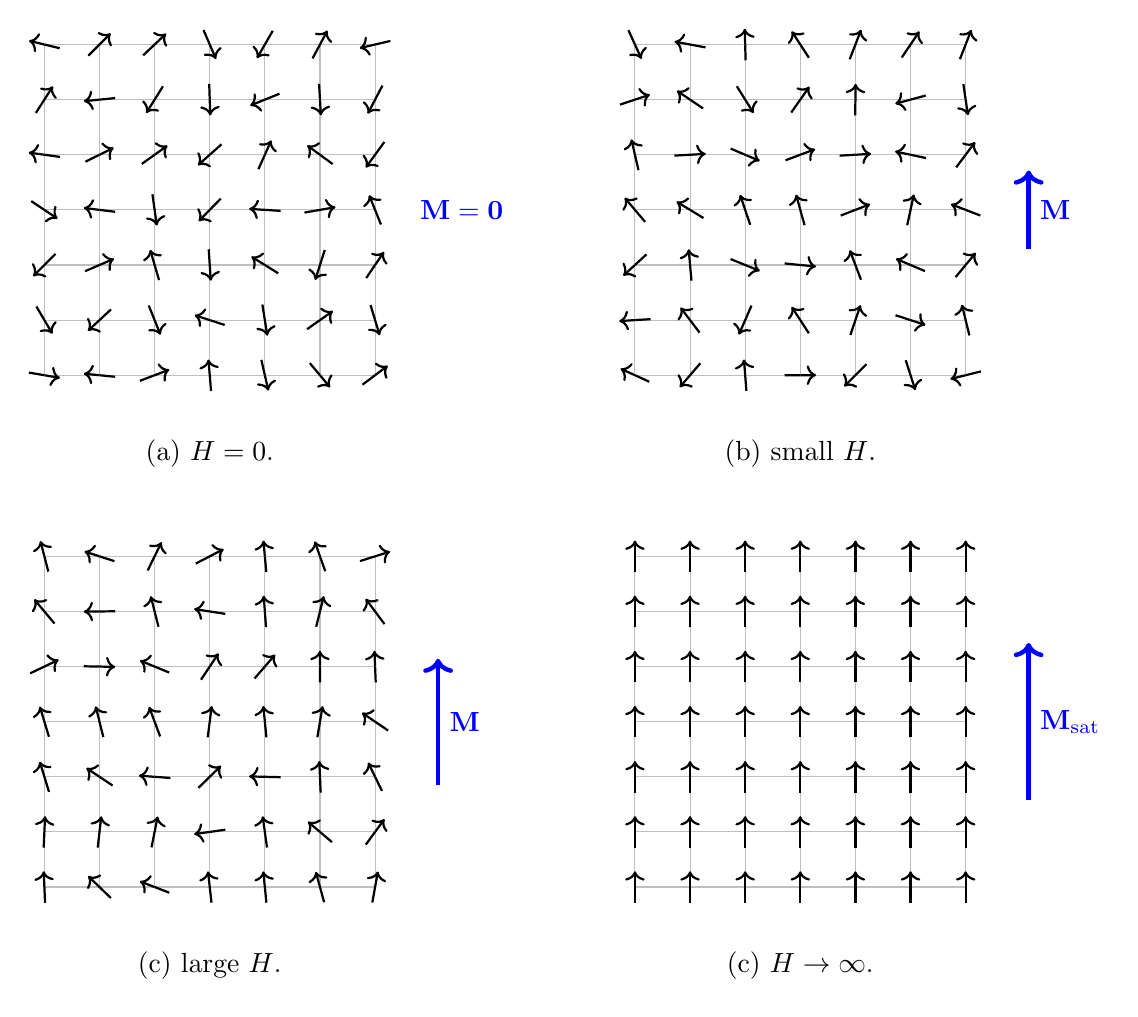
\begin{tikzpicture}
            \pgfmathsetseed{88888}
            \draw[step=0.7,thin,color=gray!50] (0,0) grid (4.2,4.2);
            \foreach \i in {0,...,6}{
                \foreach \j in {0,...,6}{
                    \tikzmath{\x = rand*180;}
                    \draw[thick] (0.7*\i,0.7*\j)--++(180+\x :0.2);
                    \draw[->,thick] (0.7*\i,0.7*\j)--++(\x :0.2);
                }
            }
            \node at (5.3,2.1)[blue]{\(\vb{M}=\vb{0}\)};
            \node at (2.1,-1){(a) \(H=0\).};
            \begin{scope}[shift={(7.5,0)}]
                \draw[step=0.7,thin,color=gray!50] (0,0) grid (4.2,4.2);
                \foreach \i in {0,...,6}{
                    \foreach \j in {0,...,6}{
                        \tikzmath{\x = rand;
                        \y = 70*\x + 110*\x*\x*\x + 90;}
                        \draw[thick] (0.7*\i,0.7*\j)--++(180+\y :0.2);
                        \draw[->,thick] (0.7*\i,0.7*\j)--++(\y :0.2);
                    }
                }
                \draw[ultra thick, blue, ->] (5,1.6)--node[right]{\(\vb{M}\)}(5,2.6);
                \node at (2.1,-1){(b) small \(H\).};
            \end{scope}
            \begin{scope}[shift={(0,-6.5)}]
                \draw[step=0.7,thin,color=gray!50] (0,0) grid (4.2,4.2);
                \foreach \i in {0,...,6}{
                    \foreach \j in {0,...,6}{
                        \tikzmath{\x = rand;
                        \y = 30*\x + 70*\x*\x*\x + 90;}
                        \draw[thick] (0.7*\i,0.7*\j)--++(180+\y :0.2);
                        \draw[->,thick] (0.7*\i,0.7*\j)--++(\y :0.2);
                    }
                }
                \draw[ultra thick, blue, ->] (5,1.3)--node[right]{\(\vb{M}\)}(5,2.9);
                \node at (2.1,-1){(c) large \(H\).};
            \end{scope}
            \begin{scope}[shift={(7.5,-6.5)}]
                \draw[step=0.7,thin,color=gray!50] (0,0) grid (4.2,4.2);
                \foreach \i in {0,...,6}{
                    \foreach \j in {0,...,6}{
                        \draw[thick] (0.7*\i,0.7*\j)--++(-90 :0.2);
                        \draw[->,thick] (0.7*\i,0.7*\j)--++(90 :0.2);
                    }
                }
                \draw[ultra thick, blue, ->] (5,1.1)--node[right]{\(\vb{M}_{\text{sat}}\)}(5,3.1);
                \node at (2.1,-1){(c) \(H\to\infty\).};
            \end{scope}
        \end{tikzpicture}
        \caption{Non-interacting magnetic moments at finite temperatures with magnetic fields upward.}
        \label{Fig:Classical_magnetisation}
    \end{figure}

    Since in a bulk material, each magnetic moment experiences an energy \(E=-\vb{\mu}\vdot\vb{H}=-\mu_z H\) in the magnetic field, and the magnetisation in other directions other that \(z\) cancels out so we have \(M=\sum \mu_z\), we can identify that\footnote{Technically, this should be Helmholtz (or Gibbs) free energy in \(NVT\) (\(NVP\)) ensembles.}
    \begin{equation}
        M=-\pdv{E}{H}\,.
    \end{equation}
    We further define the \textit{magnetic susceptibility}, \(\chi\), to be the ease that the magnetisation is generated by the magnetic field,
    \begin{equation}
        \chi\coloneqq \pdv{M}{H}=-\pdv[2]{E}{H}\,.
    \end{equation}
    By the crude analysis above, we can have the rough idea that the magnetic susceptibility is large near \(H=0\), while it decreases to \(0\) when \(H\) is very large, since then the magnetisation will reach a saturation and further increasing \(H\) will not increase \(M\) any more.
    
    \subsubsection{The Quantum View}
    Now let's proceed to the quantum mechanical view of magnetisation. Now when we impose a magnetic field of strength \(H\) along \(\vu{z}\) direction, what it does to a quantum mechanical spin is that it creates a preferred direction, or axis of quantisation. We can therefore observe the component of spins along this direction. For a particle of spin \(S\), its spin angular momentum along \(z\) direction spin governed by the spin magnetic quantum number, \(M_S\), taking values \(-S, -S+1, \dots, S\). There are in total \(2S+1\) of them. The spin angular momentum along this direction is \(S_z=\hbar M_S\). Since the field strength is \(H\), each of these levels have different energies
    \begin{equation}
        E=-\vb{\mu}\vdot\vb{H}=g\mu_{\text{B}} M_S H\,.
    \end{equation}
    The negative sign disappears because recall that the gyromagnetic ratio of electron is negative so the direction of spin is opposite to that of the magnetic moment. The magnetic field breaks the degeneracies of different \(M_S\) levels, and the energy gap between levels are proportional to \(H\).

    \begin{figure}
        \centering
        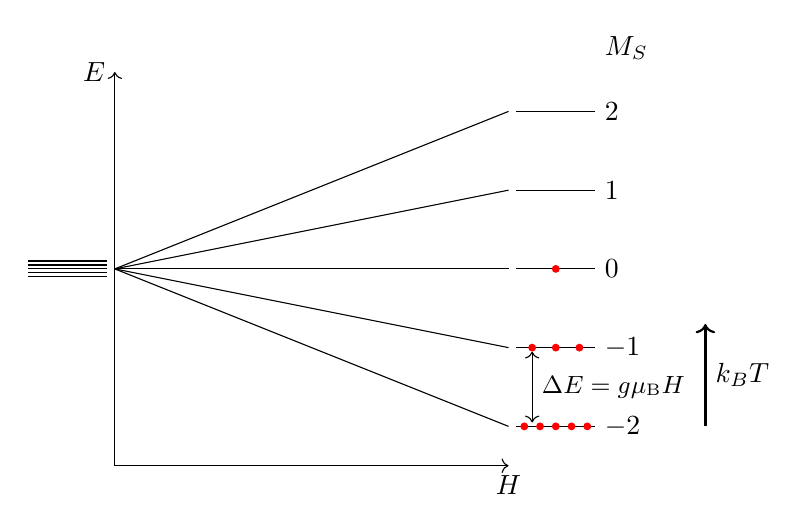
\begin{tikzpicture}
            \draw[->] (0,0)--(5,0)node[below]{\(H\)};
            \draw[->] (0,0)--(0,5)node[left]{\(E\)};
            \foreach \i in {-2,...,2}{
                \draw(0,2.5)--(5,2.5+\i);
                \draw (-1.1,2.5+0.05*\i)--(-0.1,2.5+0.05*\i);
                \draw (5.1,2.5+\i)--(6.1,2.5+\i)node[right]{\(\i\)};
            }
            \node at (6.1,5.3)[right]{\(M_S\)};
            \draw[<->](5.3,0.55)--node[right]{\small\(\Delta E=g\mu_{\text{B}}H\)}(5.3,1.45);
            \draw[thick,->] (7.5,0.5)--node[right]{\(k_B T\)}(7.5,1.8);
            \foreach \i in {-2,...,2}{
                \fill[red] (5.6+0.2*\i,0.5) circle (0.05);
            }
            \foreach \i in {-1,...,1}{
                \fill[red] (5.6+0.3*\i,1.5) circle (0.05);
            }
            \fill[red] (5.6,2.5) circle (0.05);
        \end{tikzpicture}
        \caption{External magnetic field results in the splitting of the \(M_S\) levels. The occupation of the \(M_S\) levels in the canonical ensemble follows the Boltzmann distribution.}
    \end{figure}

    The population of different \(M_S\) levels follows the Boltzmann distribution. When \(\Delta E=g\mu_{\text{B}} H\gg k_B T\), i.e. the magnetic field is large or the temperature is small, the spins will populate the lowest \(M_S\) state only. Therefore, the magnetic moments are maximally aligned with the field and we have a maximum \(\vb{M}=\vb{M}_{\text{sat}}\). If we decrease the field strength or increase the temperature, the thermal energy will be enough to promote the spins to higher \(M_S\) values, until when \(\Delta E=g\mu_{\text{B}} H\ll k_B T\), all \(M_S\) states are equally occupied, and the magnetic moments cancels so we get \(\vb{M}=\vb{0}\).

    \subsubsection{The Brillouin Function}
    We can be more quantitative. The canonical thermal average of the \(M_S\) value is
    \begin{align}
        \eval{M_S}&=\frac{\sum_{M_S=-S}^{S} M_S \ee^{-\beta E(M_S)}}{\sum_{M_S=-S}^{S} \ee^{-\beta E(M_S)}}\notag \\
        &=\frac{\sum_{M_S=-S}^{S} M_S \ee^{-\beta g\mu_{\text{B}} M_S H}}{\sum_{M_S=-S}^{S} \ee^{-\beta g\mu_{\text{B}} M_S H}}\,,
    \end{align}
    where \(\beta=1/k_B T\) is the thermodynamic inverse temperature. Denoting \(\beta g\mu_{\text{B}} H\) as \(\lambda\), this is
    \begin{align}
        \eval{M_S}&=\frac{\sum_{M_S=-S}^{S} M_S \ee^{-\lambda M_S}}{\sum_{M_S=-S}^{S} \ee^{-\lambda M_S}}\notag \\
        &=\frac{-\pdv{}{\lambda}\sum_{M_S=-S}^{S} \ee^{-\lambda M_S}}{\sum_{M_S=-S}^{S} \ee^{-\lambda M_S}}\notag \\
        &=-\pdv{}{\lambda}\ln Z(\lambda)\,,
    \end{align}
    where \(Z(\lambda)=\sum_{M_S}\ee^{-\lambda M_S}\) is the partition function. This partition function is a geometric series, evaluated to
    \begin{equation}
        Z(\lambda)=\frac{\sinh(\frac{(2S+1)\lambda}{2})}{\sinh(\frac{\lambda}{2})}\,,
    \end{equation}
    and finally this gives
    \begin{equation}
        \eval{M_S}=-\left[\frac{2S+1}{2}\coth\left(\frac{(2S+1)}{2}\lambda\right)-\frac{1}{2}\coth\left(\frac{\lambda}{2}\right)\right]\,.
    \end{equation}
    It's common to define the \textit{Brillouin function}
    \begin{equation}
        B_S(x)=\frac{2S+1}{2S}\coth\left(\frac{(2S+1)}{2S}x\right)-\frac{1}{2}\coth\left(\frac{x}{2S}\right)\,.
    \end{equation}
    This allows us to compactly write
    \begin{equation}
        \eval{M_S}=-SB_S(\lambda S)=-SB_S(\beta g\mu_{\text{B}}S H)\,.
    \end{equation}
    The molar magnetisation is therefore
    \begin{align}
        M(H, T) &= -N_A g \mu_{\text{B}}\eval{M_S}=N_A g \mu_{\text{B}} S B_S(\beta g\mu_{\text{B}}S H)\notag \\
        &=N_A g \mu_{\text{B}} S B_S\left(\frac{g\mu_{\text{B}}S}{k_B} \frac{H}{T}\right)\,.
    \end{align}
    where \(N_A\) is the Avogadro's constant.

    The magnetisation \(M\) is a function of \(\frac{H}{T}\) only, but the functional form in pretty complex. Their plots are shown in \cref{Fig:Brillouin_func}. These plots are, however, easy to interpret. As \(H/T\) increases, the molar magnetisation monotonically increases until it reaches the saturation value \(N_A g \mu_{\text{B}} S\), or \(2S\) molar Bohr magnetons taking \(g=2\). This gives us a way of measuring the spin in bulk magnetic materials.

    \begin{figure}
        \centering
        % This file was created with matplot2tikz v0.4.0.
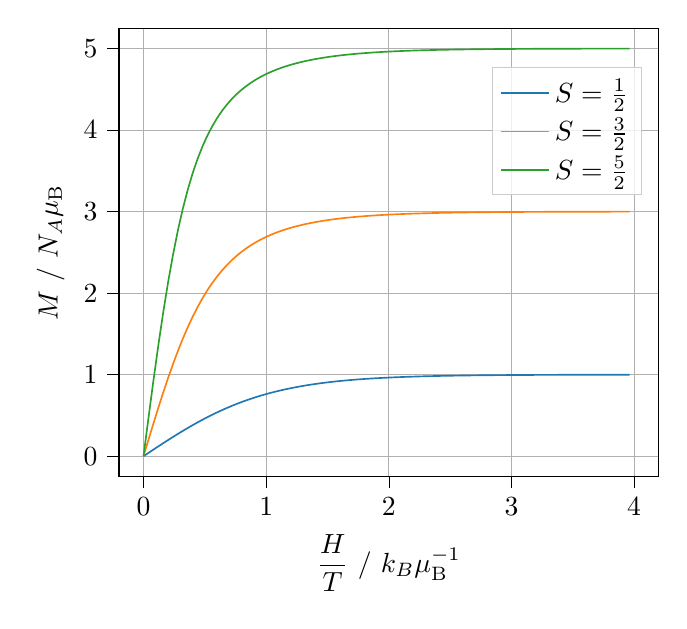
\begin{tikzpicture}

\definecolor{darkgray176}{RGB}{176,176,176}
\definecolor{darkorange25512714}{RGB}{255,127,14}
\definecolor{forestgreen4416044}{RGB}{44,160,44}
\definecolor{lightgray204}{RGB}{204,204,204}
\definecolor{steelblue31119180}{RGB}{31,119,180}

\begin{axis}[
legend cell align={left},
legend style={
  fill opacity=0.8,
  draw opacity=1,
  text opacity=1,
  at={(0.97,0.77)},
  anchor=east,
  draw=lightgray204
},
tick align=outside,
tick pos=left,
x grid style={darkgray176},
xlabel={\(\displaystyle \frac{H}{T}\) / \(\displaystyle k_B \mu_{\text{B}}^{-1}\) },
xmajorgrids,
xmin=-0.1999895, xmax=4.1999995,
xtick style={color=black},
y grid style={darkgray176},
ylabel={\(\displaystyle M\) / \(\displaystyle N_A\mu_{\text{B}}\) },
ymajorgrids,
ymin=-0.249953433730955, ymax=5.24924210842453,
ytick style={color=black}
]
\addplot [semithick, steelblue31119180]
table {%
1e-05 1.00000033853576e-05
0.0400499399399399 0.0400285403327665
0.0800898798798799 0.0799190755642059
0.12012981981982 0.11955526476503
0.16016975975976 0.158813986856416
0.2002096996997 0.19757684230597
0.24024963963964 0.235731530734823
0.28028957957958 0.273173071885133
0.32032951951952 0.309804844167731
0.360369459459459 0.345539422587116
0.400409399399399 0.380299205760097
0.440449339339339 0.414016829551124
0.480489279279279 0.446635372133679
0.520529219219219 0.478108361717756
0.560569159159159 0.508399603513739
0.600609099099099 0.537482846585722
0.640649039039039 0.565341314030664
0.680688978978979 0.591967121437393
0.720728918918919 0.61736060893463
0.760768858858859 0.641529611484504
0.800808798798799 0.664488690603608
0.840848738738739 0.686258348597395
0.880888678678679 0.706864243873452
0.920928618618619 0.72633642313831
0.960968558558558 0.744708583441805
1.0010084984985 0.762017374245393
1.04104843843844 0.778301747059531
1.08108837837838 0.793602357794332
1.12112831831832 0.807961024844575
1.16116825825826 0.821420244109127
1.2012081981982 0.834022760631165
1.24124813813814 0.845811195329749
1.28128807807808 0.856827724355468
1.32132801801802 0.867113807915651
1.36136795795796 0.876709964947284
1.4014078978979 0.88565558973565
1.44144783783784 0.89398880645176
1.48148777777778 0.901746357581712
1.52152771771772 0.908963522318369
1.56156765765766 0.915674061155857
1.6016075975976 0.921910183149198
1.64164753753754 0.927702532557095
1.68168747747748 0.933080191860988
1.72172741741742 0.938070698436296
1.76176735735736 0.94270007243322
1.8018072972973 0.946992853697771
1.84184723723724 0.950972145823939
1.88188717717718 0.954659665671765
1.92192711711712 0.958075796911516
1.96196705705706 0.961239646360128
2.002006996997 0.96416910206231
2.04204693693694 0.966880892235553
2.08208687687688 0.969390644346519
2.12212681681682 0.971712943716875
2.16216675675676 0.973861391170903
2.2022066966967 0.975848659336443
2.24224663663664 0.977686547296259
2.28228657657658 0.979386033360161
2.32232651651652 0.980957325790467
2.36236645645646 0.982409911365875
2.4024063963964 0.98375260171272
2.44244633633634 0.984993577369004
2.48248627627628 0.986140429576454
2.52252621621622 0.987200199820076
2.56256615615616 0.988179417154061
2.6026060960961 0.989084133368128
2.64264603603604 0.989919956060087
2.68268597597598 0.990692079689135
2.72272591591592 0.991405314690667
2.76276585585586 0.992064114737498
2.8028057957958 0.992672602234891
2.84284573573574 0.993234592137772
2.88288567567568 0.993753614178452
2.92292561561562 0.994232933592137
2.96296555555556 0.994675570425765
3.0030054954955 0.995084317513429
3.04304543543544 0.995461757198906
3.08308537537538 0.995810276882782
3.12312531531532 0.99613208346844
3.16316525525526 0.99642921677777
3.2032051951952 0.996703562004026
3.24324513513514 0.996956861265775
3.28328507507507 0.997190724322442
3.32332501501502 0.997406638508551
3.36336495495495 0.997605977940441
3.40340489489489 0.997790012046037
3.44344483483483 0.997959913465137
3.48348477477477 0.998116765364713
3.52352471471471 0.998261568210856
3.56356465465465 0.99839524603632
3.60360459459459 0.998518652239996
3.64364453453453 0.998632574952266
3.68368447447447 0.998737741997828
3.72372441441441 0.998834825485462
3.76376435435435 0.998924446052126
3.80380429429429 0.999007176786888
3.84384423423423 0.999083546858359
3.88388417417417 0.99915404486767
3.92392411411411 0.999219121947386
3.96396405405405 0.999279194625354
};
\addlegendentry{\(S=\frac{1}{2}\)}
\addplot [semithick, darkorange25512714]
table {%
1e-05 5.00000169267878e-05
0.0400499399399399 0.199886563704123
0.0800898798798799 0.397566544808427
0.12012981981982 0.591037214803055
0.16016975975976 0.77844175555503
0.2002096996997 0.958192361211386
0.24024963963964 1.12901828526756
0.28028957957958 1.28998710943408
0.32032951951952 1.4405010799361
0.360369459459459 1.58027301769753
0.400409399399399 1.7092877559887
0.440449339339339 1.82775532408611
0.480489279279279 1.93606144713346
0.520529219219219 2.03471974070326
0.560569159159159 2.12432859712643
0.600609099099099 2.20553445591797
0.640649039039039 2.27900207962106
0.680688978978979 2.34539167888414
0.720728918918919 2.40534223748253
0.760768858858859 2.45946013179595
0.800808798798799 2.50831205850662
0.840848738738739 2.55242131952234
0.880888678678679 2.59226661505037
0.920928618618619 2.62828262780755
0.960968558558558 2.66086181906445
1.0010084984985 2.69035698591529
1.04104843843844 2.71708424137645
1.08108837837838 2.74132617200591
1.12112831831832 2.76333500200877
1.16116825825826 2.78333565013716
1.2012081981982 2.80152860866664
1.24124813813814 2.81809260501829
1.28128807807808 2.83318702868773
1.32132801801802 2.84695412120146
1.36136795795796 2.85952093663526
1.4014078978979 2.87100108622463
1.44144783783784 2.88149628388128
1.48148777777778 2.89109771084132
1.52152771771772 2.89988721783218
1.56156765765766 2.90793838250864
1.6016075975976 2.91531743879613
1.64164753753754 2.92208409341405
1.68168747747748 2.92829224338717
1.72172741741742 2.93399060688598
1.76176735735736 2.93922327833107
1.8018072972973 2.94403021738719
1.84184723723724 2.94844768027755
1.88188717717718 2.95250860077461
1.92192711711712 2.9562429272692
1.96196705705706 2.95967792147751
2.002006996997 2.96283842360938
2.04204693693694 2.96574708817852
2.08208687687688 2.96842459407879
2.12212681681682 2.97088983206766
2.16216675675676 2.97316007238181
2.2022066966967 2.97525111485019
2.24224663663664 2.97717742356014
2.28228657657658 2.97895224786527
2.32232651651652 2.98058773129364
2.36236645645646 2.98209500971685
2.4024063963964 2.9834842999692
2.44244633633634 2.98476497995871
2.48248627627628 2.98594566118419
2.52252621621622 2.98703425446182
2.56256615615616 2.98803802956936
2.6026060960961 2.98896366943256
2.64264603603604 2.9898173194066
2.68268597597598 2.99060463214193
2.72272591591592 2.99133080846941
2.76276585585586 2.99200063469117
2.8028057957958 2.99261851662203
2.84284573573574 2.99318851068902
2.88288567567568 2.99371435236413
2.92292561561562 2.99419948217693
2.96296555555556 2.99464706952845
3.0030054954955 2.99506003450495
3.04304543543544 2.99544106787105
3.08308537537538 2.99579264940344
3.12312531531532 2.99611706471119
3.16316525525526 2.99641642067442
3.2032051951952 2.99669265962077
3.24324513513514 2.99694757234796
3.28328507507507 2.99718281009058
3.32332501501502 2.9973998955204
3.36336495495495 2.99760023286144
3.40340489489489 2.99778511719367
3.44344483483483 2.99795574301266
3.48348477477477 2.9981132121067
3.52352471471471 2.99825854080741
3.56356465465465 2.9983926666651
3.60360459459459 2.99851645459575
3.64364453453453 2.99863070254237
3.68368447447447 2.99873614669015
3.72372441441441 2.99883346627101
3.76376435435435 2.99892328799094
3.80380429429429 2.99900619010985
3.84384423423423 2.99908270620193
3.88388417417417 2.99915332862193
3.92392411411411 2.99921851170051
3.96396405405405 2.99927867469033
};
\addlegendentry{\(S=\frac{3}{2}\)}
\addplot [semithick, forestgreen4416044]
table {%
1e-05 0.000116666651592823
0.0400499399399399 0.465410730451694
0.0800898798798799 0.919916025167318
0.12012981981982 1.35397336040696
0.16016975975976 1.75992727432049
0.2002096996997 2.13259508828216
0.24024963963964 2.46930417880385
0.28028957957958 2.76958798015103
0.32032951951952 3.03468720683061
0.360369459459459 3.26699893362712
0.400409399399399 3.46957590986467
0.440449339339339 3.64572922460578
0.480489279279279 3.79874727015762
0.520529219219219 3.93171922546803
0.560569159159159 4.04744047402031
0.600609099099099 4.14837588988802
0.640649039039039 4.23666025806247
0.680688978978979 4.31412006041967
0.720728918918919 4.38230568310684
0.760768858858859 4.44252703369128
0.800808798798799 4.49588844062335
0.840848738738739 4.54332066507465
0.880888678678679 4.58560909769225
0.920928618618619 4.62341794901883
0.960968558558558 4.65731064244815
1.0010084984985 4.68776680776602
1.04104843843844 4.71519633748108
1.08108837837838 4.73995096319464
1.12112831831832 4.76233376991595
1.16116825825826 4.78260701303354
1.2012081981982 4.80099854706472
1.24124813813814 4.81770712319869
1.28128807807808 4.83290676660705
1.32132801801802 4.84675040525176
1.36136795795796 4.8593728892441
1.4014078978979 4.87089351301895
1.44144783783784 4.88141813085275
1.48148777777778 4.89104093873653
1.52152771771772 4.89984598155591
1.56156765765766 4.90790843327096
1.6016075975976 4.91529568877739
1.64164753753754 4.92206829891568
1.68168747747748 4.92828077431004
1.72172741741742 4.93398227907167
1.76176735735736 4.939217231658
1.8018072972973 4.94402582715621
1.84184723723724 4.94844449280952
1.88188717717718 4.95250628661278
1.92192711711712 4.95624124717897
1.96196705705706 4.95967670174724
2.002006996997 4.96283753810959
2.04204693693694 4.96574644533163
2.08208687687688 4.9684241273959
2.12212681681682 4.97088949327642
2.16216675675676 4.97315982643623
2.2022066966967 4.97525093630715
2.24224663663664 4.97717729394841
2.28228657657658 4.97895215377524
2.32232651651652 4.98058766299044
2.36236645645646 4.98209496013338
2.4024063963964 4.98348426397508
2.44244633633634 4.98476495382957
2.48248627627628 4.98594564221636
2.52252621621622 4.98703424069261
2.56256615615616 4.98803801957396
2.6026060960961 4.98896366217667
2.64264603603604 4.98981731413939
2.68268597597598 4.99060462831835
2.72272591591592 4.99133080569379
2.76276585585586 4.99200063267629
2.8028057957958 4.9926185151594
2.84284573573574 4.99318850962727
2.88288567567568 4.99371435159338
2.92292561561562 4.99419948161743
2.96296555555556 4.9946470691223
3.0030054954955 4.99506003421011
3.04304543543544 4.99544106765702
3.08308537537538 4.99579264924808
3.12312531531532 4.99611706459841
3.16316525525526 4.99641642059255
3.2032051951952 4.99669265956134
3.24324513513514 4.99694757230482
3.28328507507507 4.99718281005926
3.32332501501502 4.99739989549766
3.36336495495495 4.99760023284493
3.40340489489489 4.99778511718169
3.44344483483483 4.99795574300397
3.48348477477477 4.99811321210039
3.52352471471471 4.99825854080283
3.56356465465465 4.99839266666177
3.60360459459459 4.99851645459333
3.64364453453453 4.99863070254062
3.68368447447447 4.99873614668887
3.72372441441441 4.99883346627009
3.76376435435435 4.99892328799027
3.80380429429429 4.99900619010936
3.84384423423423 4.99908270620158
3.88388417417417 4.99915332862167
3.92392411411411 4.99921851170032
3.96396405405405 4.99927867469019
};
\addlegendentry{\(S=\frac{5}{2}\)}
\end{axis}

\end{tikzpicture}

        \caption{The magnetisation per mole of non-interacting spins against \(H/T\), taking \(g=2\).}
        \label{Fig:Brillouin_func}
    \end{figure}

    This high \(H/T\) limit is, however, difficult to reach since we either need a really strong magnet or a temperature close to absolute zero --- both are experimentally inaccessible. We will go to this regime in experiments only if we really need to. Instead, we are more interested in the \(H/T\to 0\) limit, since a small magnetic field and room temperature are trivially achievable.

    \subsubsection{The Curie's Law}
    If you look carefully, you can see that the \(M(\frac{H}{T})\) graph is approximately linear in the \(\frac{H}{T}\to 0\) limit, which means a constant magnetic susceptibility. The full expression of \(\chi(H, T)=\pdv{M}{H}\) needs a tough differentiation of the Brillouin function, and its full expression is meaningless to us. Instead, to look at the \(\frac{H}{T}\to 0\) limit, we only need to perform a Taylor expansion in \(\frac{H}{T}\). For small \(x\), we have \(\coth x\sim\frac{1}{x}+\frac{1}{3}x\), and substituting into the expression of \(M\), we have
    \begin{equation}
        M(H, T)=\frac{N_A g^2 \mu_{\text{B}}^2 H S(S+1)}{3k_B T}\,.
    \end{equation}
    This means that for small \(H/T\), the magnetic susceptibility is
    \begin{equation}
        \chi=\frac{M}{H}=\frac{N_A g^2 \mu_{\text{B}}^2 S(S+1)}{3k_B T}\,.
    \end{equation}
    This is independent of \(H\) (as long as \(H\) is small) and inversely proportional to \(T\). We can write this as
    \begin{equation}
        \chi=\frac{C}{T}\,,
    \end{equation}
    which is known as \textit{Curie's law}, named after Pierre Curie (not Marie Curie), where
    \begin{equation}
        C=\frac{N_A g^2 \mu_{\text{B}}^2 S(S+1)}{3 k_B}
    \end{equation}
    is \textit{Curie's constant}. This law holds when
    \begin{itemize}
        \item the ground term is well isolated from any excited terms, so only the \(2S+1\) different \(M_S\) states from the same \(S\) state are populated at the temperature considered;
        \item there are no interactions between spins.
    \end{itemize}

    Note that we have \(\chi T=C\propto S(S+1)\), and we also have \(\mu^2\propto S(S+1)\), so it is actually the macroscopic quantity \(\chi T\) that is actually measured in experiments, not the microscopic \(\mu^2\). Therefore, in figures like \cref{Fig:crossover_plot}, the proper \(y\)-axis label should actually be \(\chi T\), not \(\mu^2\).

    \subsubsection*{A Note on Units}
    Whilst much of the scientific world has moved to SI units, magnetochemists have continued to work with the cgs (centimetre-gram-second) units. There is good reason to do this since it simplifies the calculations considerably.

    Before we proceed, let's make clear of two easily confused quantities, the magnetic flux density (or magnetic induction) \(\vb{B}\) and the magnetic field strength \(\vb{H}\). What we've discussed above is the magnetic field strength \(\vb{H}\), which measures the external magnetic field generated by free currents, not counting materials' response. However, when a external field is applied to a medium, the media respond to the external field and generates a magnetisation \(\vb{M}\). This magnetisation also generates magnetic fields that can be experienced by other particles in the media, such as a moving charge or other magnetic moments. The total effect is the magnetic flux density
    \begin{equation}
        \vb{B}=\mu_0(\vb{H}+\vb{M})\,,
    \end{equation}
    where in SI units, the vacuum magnetic permeability \(\mu_0=4\pi\times 10^{-7}\unit{N}\unit{A}^{-2}\). The SI unit of \(\vb{B}\) is Tesla (\(\mathrm{T}=\mathrm{kg\ s^{-2}\ A^{-2}}\)) and the unit of \(\vb{H}\) is \(\mathrm{A\ m^{-1}}\). Therefore in vacuum, we have an annoying scaling between \(\vb{B}\) and \(\vb{H}\):
    \begin{equation}
        \vb{B}=\mu_0\vb{H}\,.
    \end{equation}

    In the cgs unit, however, we take a different convention to move this extra \(4\pi\) factor in front of \(\vb{H}\) to somewhere in the Maxwell's equations (which doesn't affect us since we don't bother solving Maxwell's equations) so that now we have
    \begin{equation}
        \vb{B}_{\text{cgs}}=\vb{H}_{\text{cgs}}+4\pi\vb{M}_{\text{cgs}}\,,
    \end{equation}
    and in vacuum, we have
    \begin{equation}
        \vb{B}_{\text{cgs}}=\vb{H}_{\text{cgs}}
    \end{equation}
    so the magnetic field and magnetic flux density now becomes the same. The cgs unit of \(\vb{B}\) is Gauss (\(\mathrm{G}\)), with \(1\unit{T}=10,000\unit{G}\), and the unit of \(\vb{H}\) is Oersted (\(\mathrm{Oe}\)), so a magnetic field of \(1\unit{Oe}\) produces a magnetic flux density \(1\unit{G}\) in vacuum. The down side is that people often forget which is the correct unit of which, and tend to use them interchangeably.

    Two additional units in the cgs system are the energy \(1\unit{erg}=10^{-7}\unit{J}\) and the \textit{electromagnetic unit} for magnetic moments \(1\unit{emu}\equiv 1\unit{erg}\unit{G}^{-1}=10^{-3}\unit{J}\unit{T}^{-1}\). One mole of Bohr magnetons is \(N_A\mu_{\text{B}}=5,585\unit{emu}\unit{mol}^{-1}\) in cgs units, and the saturation magnetisation is
    \begin{equation}
        M_{\text{sat}}=g S N_A\mu_{\text{B}}\approx 5,585gS\unit{emu}\unit{mol}^{-1}\,.
    \end{equation}
    The combination of constants \(N_A \mu_{\text{B}}^2/3k_B=0.12504\unit{emu}\unit{K}\unit{mol}^{-1}\) is coincidentally very close to \(\frac{1}{8}\) in cgs units, which allows us to approximate the Curie's constant as
    \begin{equation}
        C=\frac{N_A \mu_{\text{B}}^2}{3k_B}g^2 S(S+1)\approx \frac{1}{8}g^2 S(S+1)\unit{emu}\unit{K}\unit{mol}^{-1}
    \end{equation}
    in cgs units. If we take \(g\approx 2\), this gives us the handy formula
    \begin{equation}
        C\approx\frac{1}{2}S(S+1)\unit{emu}\unit{K}\unit{mol}^{-1}\,.
    \end{equation}

    \subsubsection{Deviation from Curie Behaviour}
    In many compounds, the magnetic susceptibility does not obey the Curie law, but instead obey a modified version
    \begin{equation}
        \chi=\frac{C}{T-\Theta}
    \end{equation}
    known as the \textit{Curie--Weiss} law for some parameter \(\Theta\) known as the \textit{Weiss constant}. This deviation from the pure Curie law can arise from a series of phenomena, including the presence of thermally accessible excited states of a single ion or some form of interaction between spin centres on neighbouring molecules. We will look at mechanisms through which they can interact later, and we will have a glimpse of how this equation arise when we introduce the Ising model. What is important is that, in both situations, there is no longer a single energy level, so our above derivation for Curie law fails.

    Suppose we have two spins, quantised along some direction in the magnetic field. There are two possibilities of their relative alignments: they are either be parallel or antiparallel. If the spins are parallel, then they are said to be in \textit{ferromagnetic alignment}, and if they are antiparallel, they are in \textit{antiferromagnetic alignment}.

    If the interaction between the two spins have an effect such that the ferromagnetic (parallel) alignment is lowered in energy than having two isolated spins and the antiferromagnetic (antiparallel) spin is raised in energy, then the two spins are said to have a \textit{ferromagnetic interaction}. This types of interaction will encourage the alignment of spins with each other, and hence all of them tends to align with the field, leading to an increased magnetic susceptibility. This will lead to a positive \(\Theta\).

    On the other hand, if the interaction between spins has an effect to encourage antiferromagnetic alignment, then this is known as an antiferromagnetic interaction, which leads to a negative \(\Theta\).

    A plot of \(\chi\), \(\chi^{-1}\) and \(\chi T\) against \(T\) are shown in \cref{Fig:Curie_Weiss}. In the \(\chi^{-1}\)-\(T\) graph, it is easy to read off the value of \(\Theta\) by the \(x\) intercept, while in the \(\chi T\)-\(T\) graph, we have \(\chi T\to T\) as \(T\to\infty\) independent of \(\Theta\), which helps us to determine the spin \(S\) (or \(g\) value) of the molecule of interest.

    \begin{figure}
        \centering
        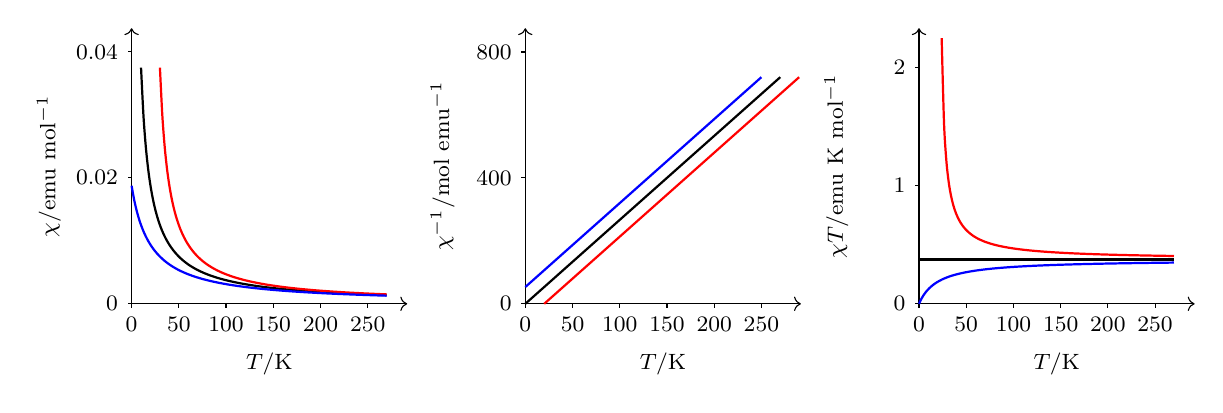
\begin{tikzpicture}
            \draw[->] (0,0)--node[below=5mm]{\footnotesize\(T/\mathrm{K}\)}(3.5,0);
            \draw[->] (0,0)--(0,3.5);
            \node[rotate=90] at (-1.05,1.75){\footnotesize\(\chi/\mathrm{emu\ mol^{-1}}\)};
            \foreach \i in {0,50,...,250}{
                \draw (0.012*\i, 0)--(0.012*\i, -0.05)node[below]{\footnotesize\(\i\)};
            }
            \foreach \i in {0,0.02,0.04}{
                \draw (0,80*\i)--(-0.05,80*\i)node[left]{\footnotesize\(\i\)};
            }
            \draw[thick,domain=10:270, smooth, variable=\x,samples=100] plot ({0.012*\x}, {80*0.375/\x});
            \draw[thick,domain=30:270, smooth, variable=\x,samples=100,red] plot ({0.012*\x}, {80*0.375/(\x-20)});
            \draw[thick,domain=0:270, smooth, variable=\x,samples=100,blue] plot ({0.012*\x}, {80*0.375/(\x+20)});

            \begin{scope}[shift={(5,0)}]
                \draw[->] (0,0)--node[below=5mm]{\footnotesize\(T/\mathrm{K}\)}(3.5,0);
                \draw[->] (0,0)--(0,3.5);
                \node[rotate=90] at (-1.05,1.75){\footnotesize\(\chi^{-1}/\mathrm{mol\ emu^{-1}}\)};
                \foreach \i in {0,50,...,250}{
                    \draw (0.012*\i, 0)--(0.012*\i, -0.05)node[below]{\footnotesize\(\i\)};
                }
                \foreach \i in {0,400,800}{
                    \draw (0,0.004*\i)--(-0.05,0.004*\i)node[left]{\footnotesize\(\i\)};
                }
                \draw[thick,domain=0:270, smooth, variable=\x,samples=100] plot ({0.012*\x}, {0.004*\x/0.375});
                \draw[thick,domain=20:290, smooth, variable=\x,samples=100,red] plot ({0.012*\x}, {0.004*(\x-20)/0.375});
                \draw[thick,domain=0:250, smooth, variable=\x,samples=100,blue] plot ({0.012*\x}, {0.004*(\x+20)/0.375});
            \end{scope}
            \begin{scope}[shift={(10,0)}]
                \draw[->] (0,0)--node[below=5mm]{\footnotesize\(T/\mathrm{K}\)}(3.5,0);
                \draw[->] (0,0)--(0,3.5);
                \node[rotate=90] at (-1.05,1.75){\footnotesize\(\chi T/\mathrm{emu\ K\ mol^{-1}}\)};
                \foreach \i in {0,50,...,250}{
                    \draw (0.012*\i, 0)--(0.012*\i, -0.05)node[below]{\footnotesize\(\i\)};
                }
                \foreach \i in {0,1,2}{
                    \draw (0,1.5*\i)--(-0.05,1.5*\i)node[left]{\footnotesize\(\i\)};
                }
                \draw[thick,domain=0:270, smooth, variable=\x,samples=100] plot ({0.012*\x}, {1.5*0.375});
                \draw[thick,domain=24:270, smooth, variable=\x,samples=100,red] plot ({0.012*\x}, {1.5*0.375*\x/(\x-20)});
                \draw[thick,domain=0:270, smooth, variable=\x,samples=100,blue] plot ({0.012*\x}, {1.5*0.375*\x/(\x+20)});
            \end{scope}
        \end{tikzpicture}
        \caption{Plot of \(\chi\), \(\chi^{-1}\) and \(\chi T\) against \(T\) for spins with \(S=\frac{1}{2}\), \(g=2\) and \(\Theta=0\unit{K}\) (black), \(\Theta=-20\unit{K}\) (antiferromagnetic, blue) and \(\Theta=+20\unit{K}\) (ferromagnetic, red).}
        \label{Fig:Curie_Weiss}
    \end{figure}

    If the ferromagnetic/antiferromagnetic interactions are too strong, then the system's behaviour will deviate from the Curie--Weiss law again. In such cases, we can still fit the Curie--Weiss law to the high temperature regime, and hence we usually linearly extrapolate the high temperature data and obtain a \(x\)-intercept to determine a suitable value of \(\Theta\).
    
    \newpage
    \section{Magnetism in Polynuclear Species}
    In this section, we will examine what happens when paramagnetic ions come into close proximity and the interactions between them becomes significant.

    \subsection{Interactions between Two Spins}
    As we mentioned before, two spins have two possible alignments --- ferromagnetic and antiferromagnetic alignments, and depending on the interactions between them, either of them may be lower in energy.
    
    \begin{figure}[ht!]
        \centering
        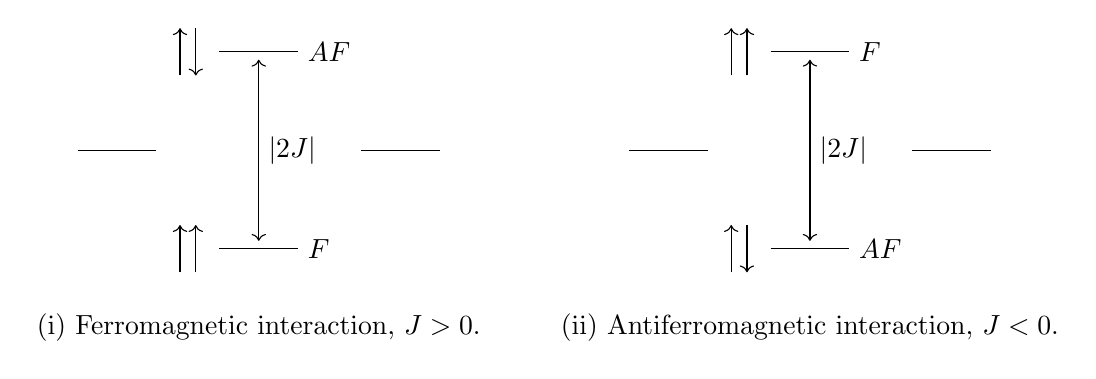
\begin{tikzpicture}
            \draw(0,0)--(1,0)node[right]{\(F\)};
            \draw(0,2.5)--(1,2.5)node[right]{\(AF\)};
            \draw[<->] (0.5,0.1)--node[right]{\(\abs{2J}\)}(0.5,2.4);
            \draw[->] (-0.5,-0.3)--(-0.5,0.3);
            \draw[->] (-0.3,-0.3)--(-0.3,0.3);
            \draw[->] (-0.5,2.2)--(-0.5,2.8);
            \draw[<-] (-0.3,2.2)--(-0.3,2.8);
            \draw (-1.8,1.25)--(-0.8,1.25);
            \draw (1.8,1.25)--(2.8,1.25);
            \node at (0.5,-1) {(i) Ferromagnetic interaction, \(J>0\).};

            \begin{scope}[shift={(7,0)}]
                \draw(0,0)--(1,0)node[right]{\(AF\)};
                \draw(0,2.5)--(1,2.5)node[right]{\(F\)};
                \draw[<->] (0.5,0.1)--node[right]{\(\abs{2J}\)}(0.5,2.4);
                \draw[->] (-0.5,-0.3)--(-0.5,0.3);
                \draw[<-] (-0.3,-0.3)--(-0.3,0.3);
                \draw[->] (-0.5,2.2)--(-0.5,2.8);
                \draw[->] (-0.3,2.2)--(-0.3,2.8);
                \draw (-1.8,1.25)--(-0.8,1.25);
                \draw (1.8,1.25)--(2.8,1.25);
                \node at (0.5,-1) {(ii) Antiferromagnetic interaction, \(J<0\).};
            \end{scope}
        \end{tikzpicture}
    \end{figure}
    
    We define the energy difference between the antiferromagnetic alignment and the ferromagnetic alignment states to be \(2J\),
    \begin{equation}
        2J = E_{\text{AF}}-E_{\text{F}}\,,
    \end{equation}
    where \(J\) is called the \textit{exchange parameter}. Then a ferromagnetic interaction has \(J>0\) while an antiferromagnetic interaction has \(J<0\).

    We've established that the main source of magnetism in ions comes from unpaired electrons, and hence the atomic orbitals with unpaired electrons are called \textit{magnetic orbitals}. How these magnetic orbitals interact determines whether the magnetic moments are coupled in a ferromagnetic or an antiferromagnetic way.

    \subsubsection{Heitler--London Model (Non-examinable)}
    The following discussion assumes familiarity of the contents in Part II A4: \textit{Theoretical Techniques}.

    Suppose we have two localised magnetic orbitals on two neighbouring ions, \(\phi_a(\vb{r})\) and \(\phi_b(\vb{r})\), each with an unpaired electron. Now we bring the two ions into proximity, so the electrons interact with the total Hamiltonian
    \begin{equation}
        \hat{H}=\hat{h}(1)+\hat{h}(2)+\frac{1}{r_{12}}
    \end{equation}
    in atomic units, where \(\hat{h}\) is the one-electron Hamiltonian. The Heitler--London model assumes the singlet (spin-antiparallel) and triplet (spin-parallel) states of the combined system to have spatial wavefunction
    \begin{align}
        \Phi_S & = \frac{\phi_a(1)\phi_b(2)+\phi_b(1)\phi_a(2)}{\sqrt{2(1+S^2)}} \\
        \Phi_T & = \frac{\phi_a(1)\phi_b(2)-\phi_b(1)\phi_a(2)}{\sqrt{2(1-S^2)}}\,,
    \end{align}
    combined with the triplet and singlet spin wavefunctions, respectively. Through some tedious algebra, the energies of the two states can be found to be
    \begin{align}
        E_S &= \expval{\hat{H}}{\Phi_S}=\frac{h_{aa}+2Sh_{ab}+h_{bb}+J+K}{1+S^2} \\
        E_T &= \expval{\hat{H}}{\Phi_T}=\frac{h_{aa}-2Sh_{ab}+h_{bb}+J-K}{1-S^2} \,,
    \end{align}
    where \(J\) is the coulomb integral and \(K\) is the exchange integral. The energy difference between the two states, expanded to order \(S^2\), is
    \begin{equation}
        E_S - E_T \approx 2K + 4Sh_{ab}\,.
    \end{equation}
    The resonance integral \(h_{ab}\) is negative, so it is common to define the \textit{hopping integral} \(t=-h_{ab}\) so that \(t\) is positive. We can recognise that the spin-antiparallel singlet state is exactly the antiferromagnetic state, and the spin-parallel triplet state is the ferromagnetic state, so we have
    \begin{equation}
        E_{\text{AF}}-E_{\text{F}}\approx2K-4St\,.
    \end{equation}
    It is conventional to write the spin coupling Hamiltonian to be \(\hat{H}=-2J\hat{\vb{S}}_1\vdot\hat{\vb{S}}_2\), and so this energy gap is \(2J\). Therefore we have
    \begin{equation}
        2J=2K-4St\,.
    \end{equation}
    Now both \(2K\) and \(4St\) are positive. The \(2K\) term comes from the exchange interaction between parallel spins, so when this term dominates, the system favours ferromagnetic alignment. This is sometimes known as the \textit{potential exchange term}. The \(4St\) terms arises from the electrons' ability to ``hop'' between atoms, which is only allowed if the electrons carry opposite spin (by Pauli exclusion principle). This leads to a reduction of the electrons' kinetic energy, and hence the system favours antiferromagnetic alignment if this term dominates. This is known as the \textit{kinetic exchange term}.

    \subsection{Direct Exchange}
    The above formula
    \begin{equation}
        2J=2K-4St
    \end{equation}
    applies when the two magnetic orbitals are close to each other so that both the exchange integral \(K\) and overlap integral \(S\) are non-negligible. This often requires the two ions to be \(\sim 4\ \text{\AA}\) apart or closer. This kind of interaction between unpaired spins by direct exchange interactions or electron hopping is known as \textit{direct exchange}. Usually, unless \(S\) in negligible for some reason (e.g. \(S=0\) due to symmetry), the kinetic term tends to dominate and the coupling tends to be antiferromagnetic.

    However, the metal ions in clusters are rarely close enough for these interactions to be significant, but still, communications between the spins are still clearly detected in many compounds. This suggests that there might be some indirect processes dominating the spin interactions in these species.

    \subsection{Superexchange}
    Superexchange is an indirect second order effect. It describes how two magnetic atoms that are far apart couple their spins through a non-magnetic atom, such as the ligand, that sits between them.
    
    Inheriting the nomenclature of the direct exchange, if a superexchange favours an antiferromagnetic state, then this is known as a kinetic superexchange, while if the ferromagnetic state is favoured, it is a potential superexchange. These are best illustrated with a few examples.

    \subsubsection{Potential Superexchange}
    Potential superexchange stabilises the ferromagnetic ground state through mutually orthogonal orbitals in the exchange pathway. This is comparatively rare, but can be achieved in several ways. The most common example is a pair of \(90^\circ\) orthogonal orbitals in \(\mathrm{M-L-M}\), where \(\mathrm{L}\) is a ligand.

    \begin{ex}
        \textit{\(90^\circ \) \(\mathrm{M}(e_g)-\mathrm{O}-\mathrm{M}(e_g)\) in \(\mathrm{[Cu(OH)_2Cu]^{2+}}\) dimer.}

        The two metal centres in the dimer are far apart, with little orbital overlap, so direct exchange is not possible.

        \begin{figure}[ht!]
            \centering
            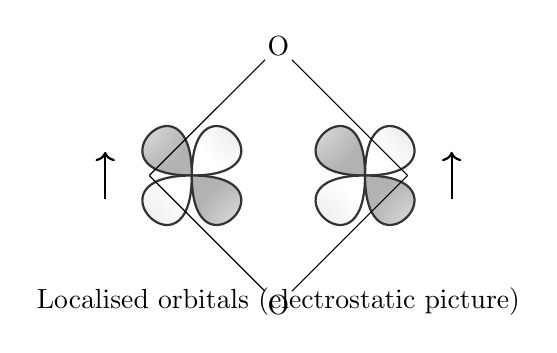
\begin{tikzpicture}
                \orbital[pos = {(-1.1,0)}, pcolor=white]{dyz}
                \orbital[pos = {(1.1,0)}, pcolor=white]{dyz}
                \node at (0,0){
                    \chemfig{[:45,2.2]O*4(--O--)}
                };
                \draw[thick,->] (-2.2,-0.3)--(-2.2,0.3);
                \draw[thick,->] (2.2,-0.3)--(2.2,0.3);

                \node at (0,-1.6) {Localised orbitals (electrostatic picture)};
            \end{tikzpicture}
        \end{figure}

        The bonding between metal and ligand is not purely ionic (crystal field theory), but instead has a significant covalent contribution. Thus the magnetic orbital on a metal may have some ligand character. As a result, the ligand bears some spin density from both metals centres and acts as a mediator for communication between the spins formally located on metals the two centres. This brings the spin polarisations on the metals closer together and allow exchange interaction happen.

        \begin{figure}[ht!]
            \centering
            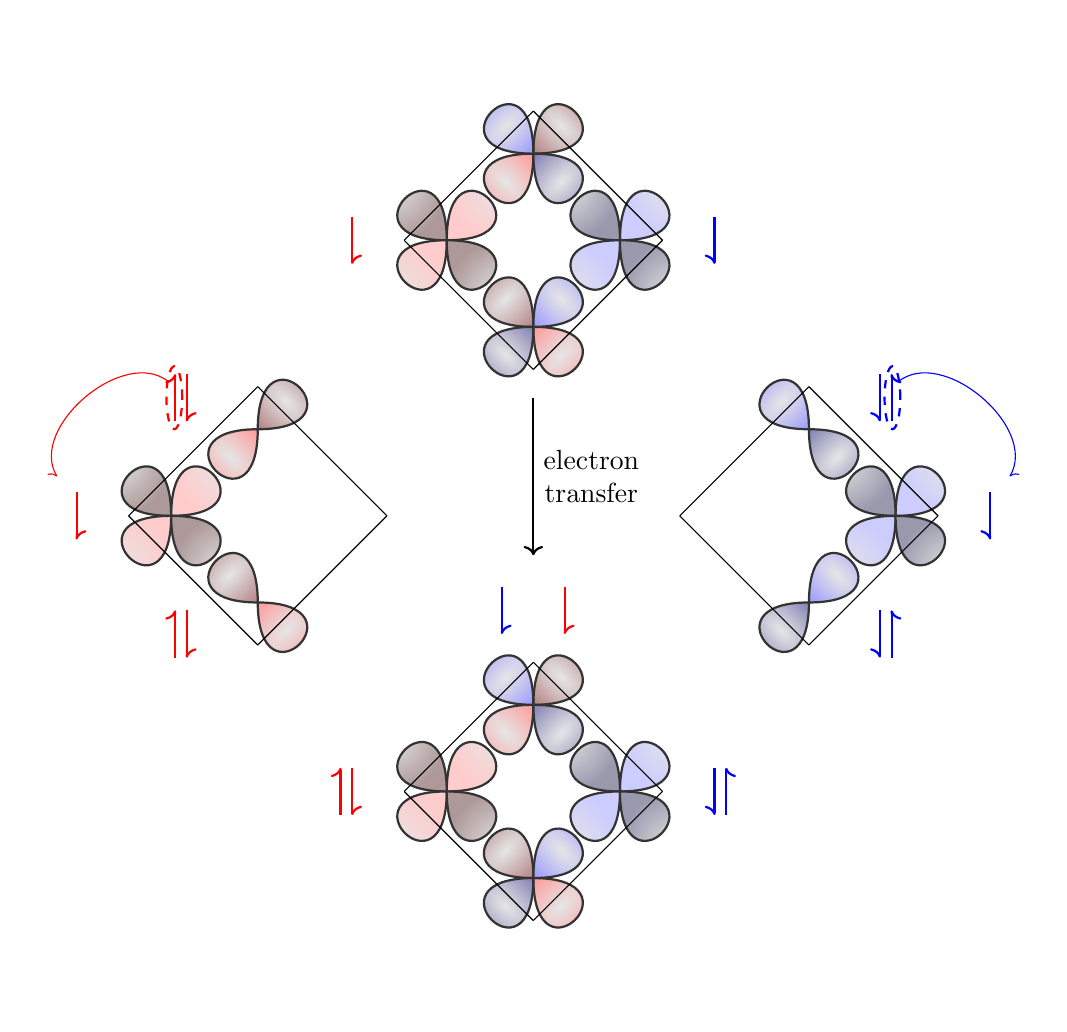
\begin{tikzpicture}
                \orbital[pos = {(-1.1,0)}, pcolor=red!20, ncolor=red!20!black!40]{dyz}
                \orbital[pos = {(1.1,0)}, pcolor=blue!20, ncolor=blue!20!black!40]{dyz}
                \node[rotate=225] at (0,1.1){\tikz{\orbital[pos = {(0,0)}, pcolor=red!40, ncolor=red!40!black!50]{py}}};
                \node[rotate=135] at (0,1.1){\tikz{\orbital[pos = {(0,0)}, pcolor=blue!40, ncolor=blue!40!black!50]{py}}};
                \node[rotate=315] at (0,-1.1){\tikz{\orbital[pos = {(0,0)}, pcolor=red!40, ncolor=red!40!black!50]{py}}};
                \node[rotate=45] at (0,-1.1){\tikz{\orbital[pos = {(0,0)}, pcolor=blue!40, ncolor=blue!40!black!50]{py}}};
                \node at (0,0){
                    \chemfig{[:45,2.2]*4(----)}
                };

                \draw[arrows = {->[left]},thick,red] (-2.3,0.3)--(-2.3,-0.3);
                \draw[arrows = {->[right]},thick,blue] (2.3,0.3)--(2.3,-0.3);

                \begin{scope}[shift={(-3.5,-3.5)}]
                    \orbital[pos = {(-1.1,0)}, pcolor=red!20, ncolor=red!20!black!40]{dyz}
                    \node[rotate=225] at (0,1.1){\tikz{\orbital[pos = {(0,0)}, pcolor=red!40, ncolor=red!40!black!50]{py}}};
                    \node[rotate=315] at (0,-1.1){\tikz{\orbital[pos = {(0,0)}, pcolor=red!40, ncolor=red!40!black!50]{py}}};
                    \node at (0,0){
                        \chemfig{[:45,2.2]*4(----)}
                    };
                    \draw[arrows = {->[left]},thick,red] (-2.3,0.3)--(-2.3,-0.3);
                    \draw[arrows = {->[left]},thick,red] (-0.9,1.8)--(-0.9,1.2);
                    \draw[arrows = {->[left]},thick,red] (-1.05,1.2)--(-1.05,1.8);
                    \draw[arrows = {->[left]},thick,red] (-0.9,-1.2)--(-0.9,-1.8);
                    \draw[arrows = {->[left]},thick,red] (-1.05,-1.8)--(-1.05,-1.2);
                    \draw[red,dashed,thick] (-1.06,1.5) ellipse (0.1 cm and 0.4 cm);
                    \draw[arrows = {->[right]},red] (-1.13,1.7) to[bend right=80] (-2.55,0.5);
                \end{scope}

                \begin{scope}[shift={(3.5,-3.5)}]
                    \orbital[pos = {(1.1,0)}, pcolor=blue!20, ncolor=blue!20!black!40]{dyz}
                    \node[rotate=135] at (0,1.1){\tikz{\orbital[pos = {(0,0)}, pcolor=blue!40, ncolor=blue!40!black!50]{py}}};
                    \node[rotate=45] at (0,-1.1){\tikz{\orbital[pos = {(0,0)}, pcolor=blue!40, ncolor=blue!40!black!50]{py}}};
                    \node at (0,0){
                        \chemfig{[:45,2.2]*4(----)}
                    };
                    \draw[arrows = {->[right]},thick,blue] (2.3,0.3)--(2.3,-0.3);
                    \draw[arrows = {->[right]},thick,blue] (0.9,1.8)--(0.9,1.2);
                    \draw[arrows = {->[right]},thick,blue] (1.05,1.2)--(1.05,1.8);
                    \draw[arrows = {->[right]},thick,blue] (0.9,-1.2)--(0.9,-1.8);
                    \draw[arrows = {->[right]},thick,blue] (1.05,-1.8)--(1.05,-1.2);
                    \draw[blue,dashed,thick] (1.06,1.5) ellipse (0.1 cm and 0.4 cm);
                    \draw[arrows = {->[left]},blue] (1.13,1.7) to[bend left=80] (2.55,0.5);
                \end{scope}

                \begin{scope}[shift={(0,-7)}]
                    \orbital[pos = {(-1.1,0)}, pcolor=red!20, ncolor=red!20!black!40]{dyz}
                    \orbital[pos = {(1.1,0)}, pcolor=blue!20, ncolor=blue!20!black!40]{dyz}
                    \node[rotate=225] at (0,1.1){\tikz{\orbital[pos = {(0,0)}, pcolor=red!40, ncolor=red!40!black!50]{py}}};
                    \node[rotate=135] at (0,1.1){\tikz{\orbital[pos = {(0,0)}, pcolor=blue!40, ncolor=blue!40!black!50]{py}}};
                    \node[rotate=315] at (0,-1.1){\tikz{\orbital[pos = {(0,0)}, pcolor=red!40, ncolor=red!40!black!50]{py}}};
                    \node[rotate=45] at (0,-1.1){\tikz{\orbital[pos = {(0,0)}, pcolor=blue!40, ncolor=blue!40!black!50]{py}}};
                    \node at (0,0){
                        \chemfig{[:45,2.2]*4(----)}
                    };

                    \draw[arrows = {->[left]},thick,red] (-2.45,-0.3)--(-2.45,0.3);
                    \draw[arrows = {->[left]},thick,red] (-2.3,0.3)--(-2.3,-0.3);
                    \draw[arrows = {->[right]},thick,blue] (2.45,-0.3)--(2.45,0.3);
                    \draw[arrows = {->[right]},thick,blue] (2.3,0.3)--(2.3,-0.3);
                    \draw[arrows = {->[left]},thick,blue] (-0.4,2.6)--(-0.4,2);
                    \draw[arrows = {->[left]},thick,red] (0.4,2.6)--(0.4,2);
                \end{scope}

                \draw[->,thick] (0,-2)--node[right,align=center]{electron\\ transfer}(0,-4);
            \end{tikzpicture}
        \end{figure}

        Note that the orbitals of the metals and ligands are divided into two orthogonal subsets --- one labelled in red and the other in blue. A simultaneous electron hopping allows the unpaired spin density to transfer to the ligand orbitals, and now these spins are close enough to have significant exchange interaction \(K\). Note that since the two ligand orbitals are orthogonal, the \(4St\) term vanishes; this orthogonality is inherited from the orthogonality of the two metal \(\mathrm{d}_{x^2-y^2}\) orbitals. Therefore, a parallel pair of spins are favoured in these ligand orbitals, which in turn favours a parallel pair of spins in the metal magnetic orbitals.

        If the electrons originally in the two metal magnetic orbitals are antiparallel, then this type of electron hopping will result in an antiparallel pair of electron on oxygen, which is disfavoured by Hund's first rule. Therefore, this type of potential superexchange results in ferromagnetic interaction.
    \end{ex}

    \subsubsection{Kinetic Superexchange}
    Kinetic superexchange stabilises the antiferromagnetic ground state through overlap of two magnetic orbitals which share the same anion orbital i.e. there is a net bonding interaction between the two magnetic orbitals.
    \begin{ex}
        \textit{\(180^\circ \) \(\mathrm{M}(e_g)-\mathrm{O}-\mathrm{M}(e_g)\) interaction.}

        Suppose now we have two magnetic \(e_g\) orbitals, but this time connected directly by a bridging \(\mathrm{O^{2-}}\) at \(180^\circ\).

        \begin{figure}[ht!]
            \centering
            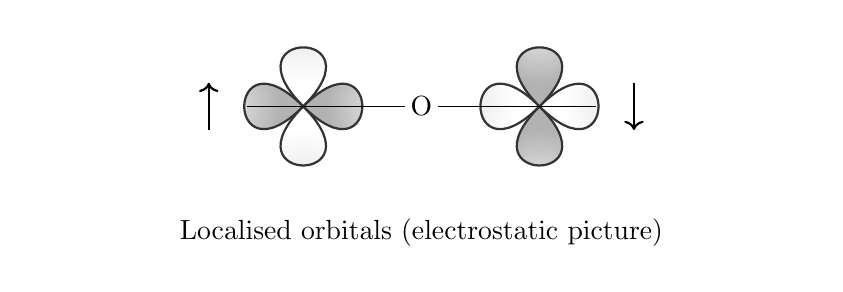
\begin{tikzpicture}
                \clip (-5,-2) rectangle (5,1);
                \node[rotate=45] at (-1.5,0){\tikz{\orbital[pos = {(0,0)}, pcolor=white]{dyz}}};
                \node[rotate=135] at (1.5,0){\tikz{\orbital[pos = {(0,0)}, pcolor=white]{dyz}}};
                \node at (0,0){
                    \chemfig{-[,2.1]O-[,2.1]}
                };
                \draw[thick,->] (-2.7,-0.3)--(-2.7,0.3);
                \draw[thick,->] (2.7,0.3)--(2.7,-0.3);

                \node at (0,-1.6) {Localised orbitals (electrostatic picture)};
                
            \end{tikzpicture}
        \end{figure}

        Again ligand-metal orbital interaction covalency enables electron transfers.
        \begin{figure}[ht!]
            \centering
            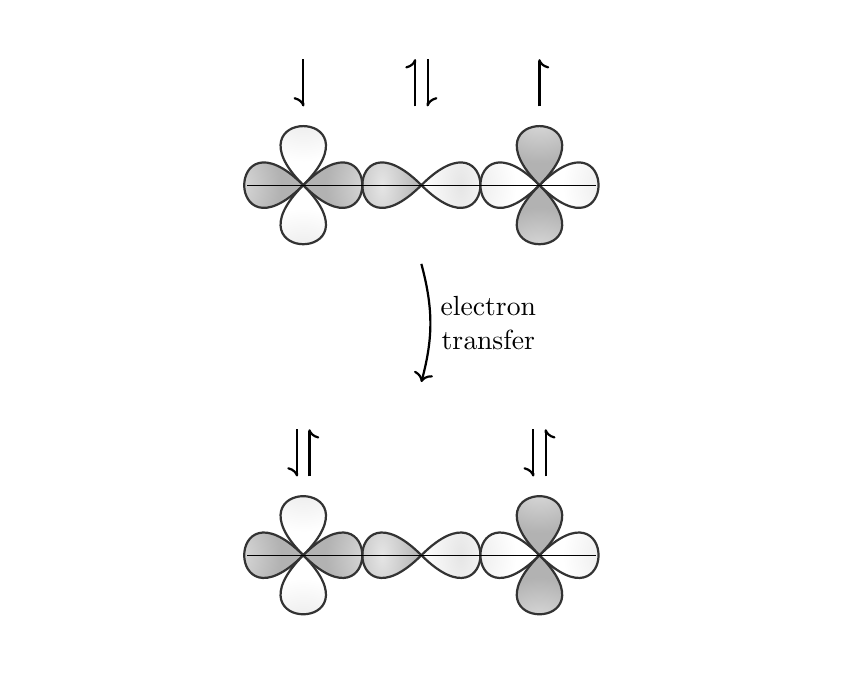
\begin{tikzpicture}
                \clip (-5,-6) rectangle (5,2);
                \node[rotate=45] at (-1.5,0){\tikz{\orbital[pos = {(0,0)}, pcolor=white]{dyz}}};
                \node[rotate=135] at (1.5,0){\tikz{\orbital[pos = {(0,0)}, pcolor=white]{dyz}}};
                \orbital[pos = {(0,0)}, pcolor=white]{py}
                \node at (0,0){
                    \chemfig{-[,2.1]-[,2.1]}
                };
                \draw[arrows = {->[right]},thick] (-1.5,1.6)--(-1.5,1);
                \draw[arrows = {->[right]},thick] (1.5,1)--(1.5,1.6);
                \draw[arrows = {->[left]},thick] (-0.08,1)--(-0.08,1.6);
                \draw[arrows = {->[left]},thick] (0.08,1.6)--(0.08,1);

                \draw[thick,->] (0,-1)to[bend left=15]node[right,align=center]{electron\\ transfer}(0,-2.5);

                \begin{scope}[shift={(0,-4.7)}]
                    \node[rotate=45] at (-1.5,0){\tikz{\orbital[pos = {(0,0)}, pcolor=white]{dyz}}};
                    \node[rotate=135] at (1.5,0){\tikz{\orbital[pos = {(0,0)}, pcolor=white]{dyz}}};
                    \orbital[pos = {(0,0)}, pcolor=white]{py}
                    \node at (0,0){
                        \chemfig{-[,2.1]-[,2.1]}
                    };
                    \draw[arrows = {->[right]},thick] (-1.58,1.6)--(-1.58,1);
                    \draw[arrows = {->[right]},thick] (1.58,1)--(1.58,1.6);
                    \draw[arrows = {->[right]},thick] (-1.42,1)--(-1.42,1.6);
                    \draw[arrows = {->[right]},thick] (1.42,1.6)--(1.42,1);
                \end{scope}
            \end{tikzpicture}
        \end{figure}

        This hopping stabilisation is only possible if the two magnetic orbitals of metals initially carries opposite spins, so it results in antiferromagnetic coupling.
    \end{ex}

    The example shown above is the \(\sigma\)-pathway of kinetic superexchange. A \(\pi\) pathway is also possible between two \(t_{2g}\) magnetic orbitals, with the arrangement shown in the figure below. This is usually weaker than the \(\sigma\) superexchange.
    \begin{figure}[ht!]
        \centering
        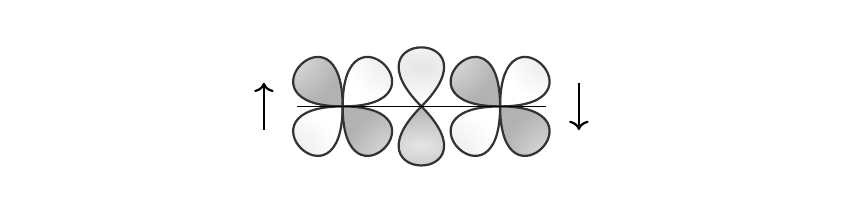
\begin{tikzpicture}
            \clip (-5,-1) rectangle (5,1);
            \orbital[pos = {(-1,0)}, pcolor=white]{dyz}
            \orbital[pos = {(1,0)}, pcolor=white]{dyz}
            \orbital[pos = {(0,0)}, pcolor=white]{pz}
            \node at (0,0){
                \chemfig{-[,1.5]-[,1.5]}
            };
            \draw[thick,->] (-2,-0.3)--(-2,0.3);
            \draw[thick,->] (2,0.3)--(2,-0.3);
            
        \end{tikzpicture}
    \end{figure}

    \subsubsection{Angular Dependence of Superexchange}
    As for the direct exchange, kinetic superexchange tends to dominate over potential superexchange unless \(S\) is small e.g. due to symmetry. As a result, the coupling constant \(J\) tends to have strong angular dependence.

    \begin{ex}
        \textit{Planar copper dimers with two hydroxyl bridges.}

        We continue investigating the following family of planar copper dimers.
        
        \begin{figure}[ht!]
            \centering
            \begin{tikzpicture}
                \clip (-5,-2) rectangle (5,2);
                \node at (0,0){
                    \chemfig{[:135,1.5]Cu*4(-O(-[,0.9]H)-Cu(-[:135]@{a}N)(-[:-135]@{b}N)-O(-[,0.9]H)-)(-[:45]@{c}N)(-[:-45]@{d}N)}
                    \chemmove{\draw[-,thick,shorten <=0.5mm, shorten >=0.5mm](a)..controls +(-135:7mm) and +(135:7mm)..(b);}
                    \chemmove{\draw[-,thick,shorten <=0.5mm, shorten >=0.5mm](c)..controls +(-45:7mm) and +(45:7mm)..(d);}
                };
            \end{tikzpicture}
            
        \end{figure}
        
        By changing the size of the \(\mathrm{N-R-N}\) ligand, we can alter the \(\mathrm{Cu-O-Cu}\) bond angle \(\theta\). When \(\theta=90^\circ\) exactly, this is the kinetic superexchange example we met before. Since the two orbitals are orthogonal, kinetic exchange is not possible so \(J\) is positive (ferromagnetic). As the bond angle deviates from \(90^\circ\), kinetic superexchange becomes possible via scheme shown in the previous example. Hence \(J\) begins to decrease.

        \begin{figure}[ht!]
            \centering
            % This file was created with matplot2tikz v0.4.0.
\begin{tikzpicture}

\definecolor{darkgray176}{RGB}{176,176,176}
\definecolor{steelblue31119180}{RGB}{31,119,180}

\begin{axis}[
tick align=outside,
tick pos=left,
x grid style={darkgray176},
xlabel={\(\displaystyle \theta\) / \(\displaystyle ^\circ\)},
xmin=88.8, xmax=115.2,
xtick style={color=black},
y grid style={darkgray176},
ylabel={\(\displaystyle 2J\) / \(\displaystyle \mathrm{cm}^{-1}\)},
ymin=-1289.49752214157, ymax=642.670431028157,
ytick style={color=black}
]
\addplot [draw=steelblue31119180, fill=steelblue31119180, mark=x, only marks, mark size=3]
table{%
x  y
95.5402423714721 178.706130417728
96.5325245872582 107.547153049391
96.9184112744514 62.2640866893312
98.682469388128 -118.867882623477
100.308708845054 -193.261459915636
102.238147328028 -354.986570004093
102.541343830572 -409.97299194447
102.92723304127 -400.269488300437
104.002205441705 -500.539124664589
107.6681352788 -714.016204833318
109.928337023874 -869.272263137848
};
\addplot [semithick, black]
table {%
90 554.844614974987
96 115.715534709139
102 -323.413545556708
108 -762.542625822556
114 -1201.6717060884
};
\end{axis}

\end{tikzpicture}

            \caption{The exchange parameter against ligand-metal bond angle for copper dimer.}
            \label{Fig:ligand_J}
        \end{figure}

        The \(J\) against \(\theta\) is plotted in \cref{Fig:ligand_J} for a range of compounds. It is found that the data shows a very good linearity against \(\theta\), with the empirical relationship
        \begin{equation}
            2J=(-74\theta + 7215)\unit{cm}^{-1}
        \end{equation}
        for \(\theta\ge 90^\circ\) measured in degrees. Since the kinetic superexchange is much stronger than potential superexchange, we only need very small spatial overlap (via ligand) for the kinetic term to dominate --- in this case \(J=0\) when \(\theta=97.5\).
    \end{ex}

    From the above example, it can be seen that the ferromagnetic coupling is fragile. The potential superexchange can be easily overwhelmed by the kinetic superexchange even with only a tiny amount of spatial overlap. It seems that it is therefore very difficult to produce ferromagnetic materials like magnets --- and even if we can make one by carefully controlling the geometry of orbital interaction, the small \(\abs{J}\) makes the ferromagnetic alignment easily scrambled by thermal activation once \(k_B T\approx \abs{J}\) at room temperatures.

    We will see how this problem is resolved when we have a magnetic network.
    
    \subsubsection{General Features of Superexchange}
    To conclude:
    \begin{itemize}
        \item The kinetic exchange pathways are usually stronger than potential superexchange. As a consequence, when competing pathways are present the resultant interaction tends to be antiferromagnetic.
        \item Because of the better overlap in \(\sigma\)-bonds, the \(\sigma\)-type superexchange tends to be greater than \(\pi\)-superexchange, i.e. the interactions involving the \(e_g\) orbitals tend to predominate. 
        \item The magnitude of \(J\) is very sensitive to orbital overlap (covalency). As a consequence \(\abs{J}\) tends to increase as we move from left to right (better energy match with ligand) or move down the group (more diffuse orbitals), and for softer and more polarisable ligands.
        \item For ions with more than one magnetic orbitals, both \(\sigma\) and \(\pi\) type interactions are possible.
    \end{itemize}
    
    \subsection{Magnetic Susceptibility of Clusters}
    Magnetic coupling makes the susceptibility of clusters deviate from the simple Curie law --- and the resulting general expression of \(\chi\) is usually quite complicated: coupling splits the system to a number of energy levels, with population given by the Boltzmann distribution, and each contributes accordingly to the total magnetic susceptibility. We will first investigate the high temperature and low temperature limits, which are quite easy to work out, before discussing how to find the general expression of \(\chi(T)\) for a cluster.

    \subsubsection{High Temperature Limit}
    If the temperature is high enough with \(k_B T\gg \abs{J}\), we can simply ignore the coupling and act as if the spin carriers are non-interacting. If the cluster carries spins \(\{S_1,\dots,S_n\}\), the molar susceptibility of the cluster is therefore the sum of the molar susceptibility of the individual spin carriers in the ideal Curie case,
    \begin{equation}
        \chi T=\sum_{i=1}^{n}\frac{N_A g^2 \mu_{\text{B}}^2}{3k_B} S_i (S_i+1)\,.
    \end{equation}
    If we use \(g\approx 2.0\), this gives
    \begin{equation}
        \chi T\approx\sum_{i=1}^{n}\frac{1}{2}S_i (S_i+1)\unit{emu}\unit{K}\unit{mol}^{-1}
    \end{equation}
    in cgs units.

    \subsubsection{Low Temperature Limit}
    Now, if \(k_B T\ll\abs{J}\), only the overall magnetic ground state is occupied. The whole cluster acts as like a single spin carrier with total spin \(S_{\text{T}}\), so that
    \begin{equation}
        \chi T=\frac{N_A g^2 \mu_{\text{B}}^2}{3k_B} S_{\text{T}} (S_{\text{T}}+1)\approx \frac{1}{2}S_{\text{T}}(S_{\text{T}}+1)\unit{emu}\unit{K}\unit{mol}^{-1}\,.
    \end{equation}
    Note that to use Curie law, we must have \(\frac{H}{T} / k_B\mu_{\text{B}}^{-1}\ll 1\) so that we are in the linear region of Brillouin's function. Since we take \(T\) to be small, \(H\) needs to small as well.


    The total spin \(S_{\text{T}}\) for the magnetic ground state varies from case to case. If all the coupling within the cluster is ferromagnetic, the magnetic ground state clearly has all spins aligned so
    \begin{equation}
        S_{\text{T}}=\sum_{i=1}^{n}S_i\,.
    \end{equation}
    If we have a chain of \(n\) identical spins \(S\), then the magnetic ground state has the spins alternating in direction. If \(n\) is even, then the ground states have all spins cancelled out so \(S_{\text{T}}=0\), and hence
    \begin{equation}
        \chi T =0\,.
    \end{equation}
    If \(n\) is odd, then we have all spins cancelled except one spin left out so \(S_{\text{T}}=S\) and
    \begin{equation}
        \chi T=\frac{N_A g^2 \mu_{\text{B}}^2}{3k_B} S(S+1)\,.
    \end{equation}
    If the coupling geometry is any more complex, then we need to find ground state \(S_{\text{T}}\) \textit{ad hoc}.

    \begin{ex}
        \textit{\(\mathrm{Ni_{12}(chp)_{12}(OAc)_{12}(H_2O)_6(thf)_6}\).}

        This complex contains twelve octahedral \(\mathrm{Ni(II)}\) ions with \(S=1\). Using \(g=2.0\), we get the high temperature (non-interacting limit)
        \begin{equation}
            \lim_{T\to\infty}\chi T\approx 12\times\frac{1}{2}S(S+1)=12\unit{emu}\unit{K}\unit{mol}^{-1}\,.
        \end{equation}
        If the metal centres are ferromagnetically coupled, then the low temperature has \(S_{\text{T}}=12\) and
        \begin{equation}
            \lim_{T\to 0}\chi_{\text{ferro}} T \approx \frac{1}{2}S_{\text{T}}(S_{\text{T}} + 1)=78\unit{emu}\unit{K}\unit{mol}^{-1}\,,
        \end{equation}
        while if the nickel centres are antiferromagnetically coupled, the ground state has \(S_{\text{T}}=0\) and
        \begin{equation}
            \lim_{T\to 0}\chi_{\text{anti}} T \approx \frac{1}{2}S_{\text{T}}(S_{\text{T}} + 1)=0\unit{emu}\unit{K}\unit{mol}^{-1}\,.
        \end{equation}

        We have the experimental data in \cref{Fig:Ni12cluster}. We see that the cluster's \(\chi T\) value increases as temperature decreases, so the coupling between \(\mathrm{Ni}\) centres must be ferromagnetic. However, we found that the high temperature \(\chi T\) value levels of at around \(18\unit{emu}\unit{K}\unit{mol}^{-1}\), which is larger than our calculated value of \(12\unit{emu}\unit{K}\unit{mol}^{-1}\). This means that in this compound, we actually have a \(g\) value larger than \(2.0\): usually for \(\mathrm{Ni^{2+}}\), \(g\approx 2.2\) is a good approximation, while fitting this set of data gives \(g\approx 2.45\).

        What we can also observe is that the \(\chi T\) value does not reach its low temperature limit even for the lowest-temperature data measured (\(1.8\unit{K}\)). This again suggests that the ferromagnetic coupling in this compound is really weak. Magnetic excited states with \(S_{\text{T}}<12\) have significant populations even at \(1.8\unit{K}\).

        \begin{figure}
            \centering
            \begin{subfigure}[h]{0.4\linewidth}
                \begin{adjustbox}{width=\linewidth}
                \includegraphics[width=\linewidth]{figures/Ni_cluster.jpg}
                \end{adjustbox}
            \end{subfigure}
            \hskip 0.8cm
            \begin{subfigure}[h]{0.48\linewidth}
                \begin{adjustbox}{width=\linewidth}
                % This file was created with matplot2tikz v0.4.0.
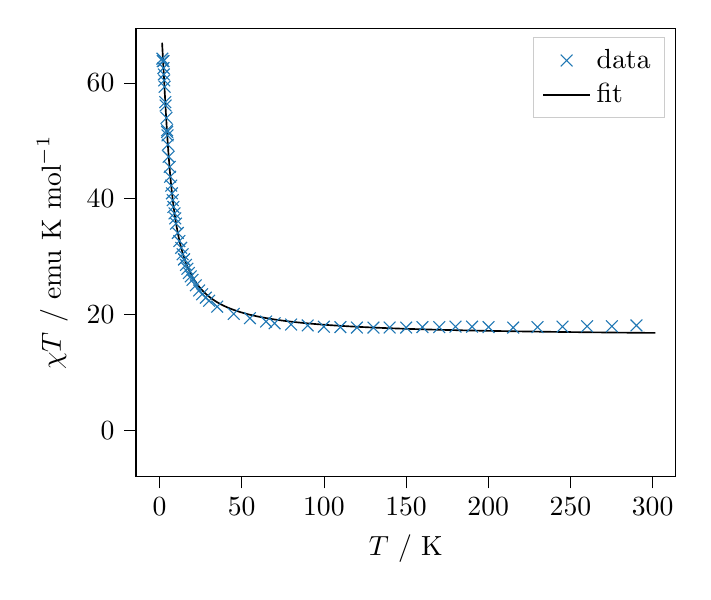
\begin{tikzpicture}

\definecolor{darkgray176}{RGB}{176,176,176}
\definecolor{lightgray204}{RGB}{204,204,204}
\definecolor{steelblue31119180}{RGB}{31,119,180}

\begin{axis}[
legend cell align={left},
legend style={fill opacity=0.8, draw opacity=1, text opacity=1, draw=lightgray204},
tick align=outside,
tick pos=left,
x grid style={darkgray176},
xlabel={\(\displaystyle T\) / \(\displaystyle \mathrm{K}\)},
xmin=-14.2673360837386, xmax=314,
xtick style={color=black},
y grid style={darkgray176},
ylabel={\(\displaystyle \chi T\) / \(\displaystyle \mathrm{emu\ K\ mol^{-1}}\)},
ymin=-8, ymax=69.4399923644874,
ytick style={color=black}
]
\addplot [draw=steelblue31119180, fill=steelblue31119180, mark=x, only marks, mark size=3]
table{%
x  y
1.78971258585885 64.1850677875314
2.01342281879195 63.7434274089825
2.46085352545617 63.7434274089825
2.46085352545617 62.5657191712774
2.68456375838926 61.4616182249051
2.90828423212039 60.4311228851415
3.13199446505348 59.3270219387692
3.5794251717177 56.6771796674758
7.60627080930159 40.9253406223815
4.25056611131502 53.9537317895739
4.69798657718121 51.819135503438
4.69798657718121 51.524709707555
4.92170705091233 50.9358547463402
5.14541728384543 49.3165078148105
5.59284799050965 47.2555205047319
6.26398893010696 45.4889589905363
6.48769916304006 43.7960030829493
7.15884010263737 42.2502617580282
10.0671140939597 35.6992616864033
3.8031354046508 56.0883280757098
8.05369127516779 39.7476340694006
8.50112198183201 38.5699241469711
9.17226292142932 37.4658232005989
9.61969362809354 36.5825424435011
11.1856857402213 34.0799113854249
12.0805369127517 32.6813880126183
13.1991085590132 31.5036780901888
14.0939597315436 30.3995771438165
14.9888211448721 29.5162963867188
14.9888211448721 29.5162963867188
16.1073825503356 28.5594066535637
17.002243963664 27.8969460857403
17.8970951361944 27.1608832807571
19.015666782456 26.5720249500936
20.1342281879195 25.9831733583276
22.1476510067114 25.0262836251725
24.1610738255034 24.1430028680747
25.9507966521602 23.4805423002514
28.1879194630873 22.8916907084853
30.2013422818792 22.3764413538791
35.1230493327915 21.3459493835642
45.1901634267513 20.0946372239748
55.0335570469799 19.3585676800941
64.8769711488045 18.7697160883281
70.0223781918519 18.4752869229964
80.0894922858117 18.2544667337219
90.1566063797714 18.1072555205047
100 17.8864353312303
110.06711409396 17.812826355173
120.134228187919 17.7392173791157
130.201342281879 17.7392173791157
140.044756383704 17.7392173791157
150.111870477664 17.7392173791157
159.955264097892 17.812826355173
170.246098665583 17.812826355173
180.089492285812 17.8864353312303
190.156606379771 17.8864353312303
200.223740955327 17.812826355173
215.212541618603 17.7392173791157
229.977642289744 17.812826355173
245.190183908347 17.8864353312303
260.178984571623 17.9600375683902
275.167785234899 17.9600375683902
290.156626861367 18.1072555205047
};
\addlegendentry{data}
\addplot [semithick, black]
table {%
1.61074132727297 66.9319803146216
2.40663493183495 62.8305653420207
3.20252853639693 58.5001329795362
3.99842214095891 54.371747669754
4.7943157455209 50.6511544281558
5.59020935008288 47.394287018777
6.38610295464486 44.5794363356388
7.18199655920685 42.1549804653983
7.97789016376883 40.0634452041015
8.77378376833081 38.2515230924775
9.5696773728928 36.6732721388405
10.3655709774548 35.2903921571955
11.1614645820168 34.0714194523025
11.9573581865787 32.9906399714031
12.7532517911407 32.0270387295577
13.5491453957027 31.1633917104693
14.3450390002647 30.3855188605119
15.1409326048267 29.6816840125024
15.9368262093887 29.0421181006506
16.7327198139506 28.4586418558691
17.5286134185126 27.9243672300322
18.3245070230746 27.4334605634053
19.1204006276366 26.9809540157831
19.9162942321986 26.5625947309386
20.7121878367606 26.1747235685183
21.5080814413225 25.8141770873314
22.3039750458845 25.4782078928859
23.0998686504465 25.1644195592136
23.8957622550085 24.8707131759014
24.6916558595705 24.5952432160661
25.4875494641325 24.3363809165915
26.2834430686944 24.0926837440704
27.0793366732564 23.862869815709
27.8752302778184 23.6457963744382
28.6711238823804 23.4404415971241
29.4670174869424 23.2458891557506
30.2629110915044 23.0613150626298
31.0588046960663 22.8859764187824
31.8546983006283 22.7192017547676
32.6505919051903 22.560382709332
33.4464855097523 22.4089668363219
34.2423791143143 22.2644513666794
35.0382727188763 22.1263777818302
35.8341663234382 21.9943270787752
36.6300599280002 21.8679156268188
37.4259535325622 21.7467915319653
38.2218471371242 21.6306314382825
39.0177407416862 21.5191377064956
39.8136343462482 21.4120359191794
40.6095279508101 21.3090726694928
41.4054215553721 21.2100135967387
42.2013151599341 21.114641637336
42.9972087644961 21.0227554642613
43.7931023690581 20.9341680917817
44.5889959736201 20.8487056254896
45.384889578182 20.7662061403545
46.180783182744 20.6865186718081
46.976676787306 20.6095023068431
47.772570391868 20.5350253637865
48.56846399643 20.4629646508492
49.364357600992 20.3932047947902
50.1602512055539 20.3256376321063
50.9561448101159 20.2601616560745
51.7520384146779 20.196681513778
52.5479320192399 20.1351075479363
53.3438256238019 20.0753553789641
54.1397192283638 20.0173455232077
54.9356128329258 19.9610030437669
55.7315064374878 19.9062572307108
56.5274000420498 19.8530413078465
57.3232936466118 19.8012921635112
58.1191872511738 19.7509501031256
58.9150808557357 19.7019586214888
59.7109744602977 19.6542641930061
60.5068680648597 19.6078160782249
61.3027616694217 19.5625661452225
62.0986552739837 19.5184687045348
62.8945488785457 19.4754803564458
63.6904424831076 19.4335598495715
64.4863360876696 19.3926679497806
65.2822296922316 19.3527673185783
66.0781232967936 19.3138224001717
66.8740169013556 19.2757993164988
67.6699105059176 19.2386657695783
68.4658041104795 19.2023909505906
69.2616977150415 19.1669454551551
70.0575913196035 19.1323012043194
70.8534849241655 19.0984313708143
71.6493785287275 19.0653103101727
72.4452721332894 19.0329134963405
73.2411657378514 19.0012174614434
74.0370593424134 18.9701997393998
74.8329529469754 18.9398388130967
75.6288465515374 18.910114064869
76.4247401560994 18.881005730044
77.2206337606613 18.8524948533324
78.0165273652233 18.8245632478645
78.8124209697853 18.7971934566865
79.6083145743473 18.7703687165462
80.4042081789093 18.7440729238117
81.2001017834713 18.7182906023774
81.9959953880333 18.6930068734236
82.7918889925952 18.6682074269071
83.5877825971572 18.6438784946665
84.3836762017192 18.6200068250393
85.1795698062812 18.5965796588895
85.9754634108432 18.573584706958
86.7713570154051 18.5510101284499
87.5672506199671 18.5288445107811
88.3631442245291 18.5070768504118
89.1590378290911 18.4856965346993
89.9549314336531 18.4646933247076
90.7508250382151 18.4440573389156
91.546718642777 18.4237790377695
92.342612247339 18.4038492090286
93.138505851901 18.3842589538582
93.934399456463 18.3649996736243
94.730293061025 18.3460630573504
95.5261866655869 18.3274410697975
96.3220802701489 18.3091259401313
97.1179738747109 18.2911101511433
97.9138674792729 18.2733864289949
98.7097610838349 18.2559477334548
99.5056546883969 18.2387872486016
100.301548292959 18.2218983739673
101.097441897521 18.2052747160971
101.893335502083 18.1889100805012
102.689229106645 18.172798463981
103.485122711207 18.1569340473056
104.281016315769 18.1413111882233
105.076909920331 18.1259244147879
105.872803524893 18.110768418986
106.668697129455 18.0958380506469
107.464590734017 18.0811283116222
108.260484338579 18.0666343502211
109.056377943141 18.0523514558884
109.852271547703 18.038275054112
110.648165152265 18.0244007015497
111.444058756827 18.0107240813643
112.239952361389 17.9972409987551
113.035845965951 17.9839473766788
113.831739570513 17.9708392517475
114.627633175075 17.9579127702987
115.423526779637 17.9451641846255
116.219420384199 17.9325898493622
117.01531398876 17.920186218016
117.811207593322 17.9079498396396
118.607101197884 17.8958773556363
119.402994802446 17.8839654966931
120.198888407008 17.8722110798345
120.99478201157 17.8606110055928
121.790675616132 17.8491622552887
122.586569220694 17.8378618884168
123.382462825256 17.826707040133
124.178356429818 17.8156949188375
124.97425003438 17.8048228038499
125.770143638942 17.7940880431722
126.566037243504 17.7834880513361
127.361930848066 17.7730203073307
128.157824452628 17.7626823526071
128.95371805719 17.7524717891563
129.749611661752 17.7423862776586
130.545505266314 17.7324235356989
131.341398870876 17.7225813360482
132.137292475438 17.7128575050065
132.93318608 17.7032499208041
133.729079684562 17.6937565120616
134.524973289124 17.6843752563025
135.320866893686 17.6751041785198
136.116760498248 17.6659413497913
136.91265410281 17.6568848859443
137.708547707372 17.6479329462653
138.504441311934 17.6390837322552
139.300334916496 17.6303354864259
140.096228521058 17.6216864911389
140.89212212562 17.6131350674821
141.688015730182 17.6046795741854
142.483909334744 17.5963184065717
143.279802939306 17.5880499955428
144.075696543868 17.5798728065998
144.87159014843 17.5717853388944
145.667483752992 17.563786124312
146.463377357554 17.5558737265844
147.259270962116 17.5480467404314
148.055164566678 17.5403037907293
148.85105817124 17.5326435317074
149.646951775802 17.5250646461681
150.442845380364 17.5175658447339
151.238738984926 17.5101458651164
152.034632589488 17.5028034714088
152.83052619405 17.4955374534007
153.626419798612 17.4883466259139
154.422313403174 17.4812298281584
155.218207007736 17.474185923109
156.014100612298 17.4672137968999
156.80999421686 17.4603123582386
157.605887821422 17.4534805378366
158.401781425984 17.4467172878584
159.197675030546 17.4400215813859
159.993568635108 17.4333924118991
160.78946223967 17.4268287927725
161.585355844232 17.4203297567863
162.381249448794 17.4138943556511
163.177143053356 17.4075216595478
163.973036657918 17.4012107566799
164.768930262479 17.3949607528391
165.564823867041 17.3887707709833
166.360717471603 17.3826399508268
167.156611076165 17.3765674484422
167.952504680727 17.3705524358733
168.748398285289 17.3645941007594
169.544291889851 17.3586916459699
170.340185494413 17.3528442892488
171.136079098975 17.3470512628699
171.931972703537 17.3413118133008
172.727866308099 17.3356252008764
173.523759912661 17.3299906994816
174.319653517223 17.3244075962428
175.115547121785 17.3188751912268
175.911440726347 17.313392797149
176.707334330909 17.3079597390891
177.503227935471 17.302575354214
178.299121540033 17.297238991509
179.095015144595 17.2919500115151
179.890908749157 17.2867077860742
180.686802353719 17.2815116980801
181.482695958281 17.2763611412372
182.278589562843 17.2712555198245
183.074483167405 17.2661942484658
183.870376771967 17.2611767519071
184.666270376529 17.2562024647976
185.462163981091 17.2512708314784
186.258057585653 17.2463813057756
187.053951190215 17.2415333507986
187.849844794777 17.2367264387438
188.645738399339 17.2319600507032
189.441632003901 17.227233676478
190.237525608463 17.2225468143964
191.033419213025 17.2178989711365
191.829312817587 17.2132896615531
192.625206422149 17.2087184085091
193.421100026711 17.2041847427112
194.216993631273 17.1996882025489
195.012887235835 17.1952283339385
195.808780840397 17.1908046901701
196.604674444959 17.1864168317583
197.400568049521 17.1820643262972
198.196461654083 17.1777467483184
198.992355258645 17.173463679152
199.788248863207 17.1692147067919
200.584142467769 17.1649994257635
201.380036072331 17.1608174369948
202.175929676893 17.1566683476906
202.971823281455 17.1525517712097
203.767716886017 17.1484673269447
204.563610490579 17.1444146402049
205.359504095141 17.1403933421015
206.155397699703 17.1364030694363
206.951291304265 17.132443464592
207.747184908827 17.1285141754253
208.543078513389 17.1246148551631
209.338972117951 17.1207451623001
210.134865722513 17.1169047604994
210.930759327074 17.1130933184949
211.726652931636 17.1093105099962
212.522546536198 17.1055560135958
213.31844014076 17.1018295126775
214.114333745322 17.0981306953283
214.910227349884 17.0944592542505
215.706120954446 17.0908148866775
216.502014559008 17.0871972942901
217.29790816357 17.0836061831351
218.093801768132 17.080041263546
218.889695372694 17.0765022500652
219.685588977256 17.0729888613675
220.481482581818 17.069500820186
221.27737618638 17.0660378532388
222.073269790942 17.062599691158
222.869163395504 17.0591860684196
223.665057000066 17.0557967232756
224.460950604628 17.0524313976866
225.25684420919 17.0490898372567
226.052737813752 17.0457717911696
226.848631418314 17.0424770121252
227.644525022876 17.0392052562791
228.440418627438 17.0359562831815
229.236312232 17.0327298557191
230.032205836562 17.0295257400572
230.828099441124 17.0263437055832
231.623993045686 17.023183524851
232.419886650248 17.0200449735276
233.21578025481 17.0169278303392
234.011673859372 17.0138318770197
234.807567463934 17.0107568982598
235.603461068496 17.007702681657
236.399354673058 17.0046690176664
237.19524827762 17.0016556995535
237.991141882182 16.9986625233467
238.787035486744 16.9956892877913
239.582929091306 16.9927357943049
240.378822695868 16.9898018469326
241.17471630043 16.9868872523042
241.970609904992 16.9839918195914
242.766503509554 16.9811153604662
243.562397114116 16.9782576890603
244.358290718678 16.9754186219249
245.15418432324 16.9725979779914
245.950077927802 16.9697955785333
246.745971532364 16.9670112471279
247.541865136926 16.9642448096198
248.337758741488 16.9614960940843
249.13365234605 16.9587649307919
249.929545950612 16.9560511521734
250.725439555174 16.9533545927855
251.521333159736 16.9506750892776
252.317226764298 16.9480124803582
253.11312036886 16.9453666067631
253.909013973422 16.9427373112234
254.704907577984 16.9401244384344
255.500801182546 16.937527835025
256.296694787108 16.9349473495277
257.092588391669 16.9323828323495
257.888481996232 16.9298341357422
258.684375600793 16.9273011137749
259.480269205355 16.9247836223056
260.276162809917 16.9222815189544
261.072056414479 16.9197946630759
261.867950019041 16.9173229157335
262.663843623603 16.9148661396734
263.459737228165 16.9124241992989
264.255630832727 16.909996960646
265.051524437289 16.9075842913584
265.847418041851 16.9051860606636
266.643311646413 16.9028021393496
267.439205250975 16.9004323997411
268.235098855537 16.8980767156773
269.030992460099 16.8957349624893
269.826886064661 16.8934070169778
270.622779669223 16.8910927573922
271.418673273785 16.8887920634086
272.214566878347 16.8865048161096
273.010460482909 16.8842308979633
273.806354087471 16.8819701928036
274.602247692033 16.8797225858103
275.398141296595 16.8774879634894
276.194034901157 16.8752662136544
276.989928505719 16.8730572254073
277.785822110281 16.8708608891201
278.581715714843 16.868677096417
279.377609319405 16.8665057401561
280.173502923967 16.8643467144123
280.969396528529 16.8621999144599
281.765290133091 16.8600652367556
282.561183737653 16.8579425789222
283.357077342215 16.8558318397316
284.152970946777 16.8537329190894
284.948864551339 16.8516457180188
285.744758155901 16.8495701386448
286.540651760463 16.8475060841793
287.336545365025 16.845453458906
288.132438969587 16.8434121681653
288.928332574149 16.8413821183399
289.724226178711 16.839363216841
290.520119783273 16.8373553720932
291.316013387835 16.8353584935218
292.111906992397 16.8333724915381
292.907800596959 16.8313972775269
293.703694201521 16.8294327638328
294.499587806083 16.8274788637475
295.295481410645 16.8255354914968
296.091375015207 16.8236025622283
296.887268619769 16.8216799919988
297.683162224331 16.8197676977625
298.479055828893 16.8178655973588
299.274949433455 16.8159736095005
300.070843038017 16.8140916537622
300.866736642579 16.8122196505693
301.662630247141 16.8103575211862
};
\addlegendentry{fit}
\end{axis}

\end{tikzpicture}

                \end{adjustbox}
            \end{subfigure}
            \caption{The structure and the measured and fitted \(\chi T\) against \(T\) for the \(\mathrm{Ni_{12}}\) cluster.}
            \label{Fig:Ni12cluster}
        \end{figure}
    \end{ex}

    \begin{ex}
        \textit{\(\mathrm{Cu_2(OAc)_4\cdot 2H_2O}\).}

        This cluster contains two \(S=\frac{1}{2}\) \(\mathrm{Cu(II)}\) ions. Using \(g=2.0\), the high temperature limit is
        \begin{equation}
            \lim_{T\to\infty}\chi T\approx 2\times\frac{1}{2}S(S+1)=0.75\unit{emu}\unit{K}\unit{mol}^{-1}\,.
        \end{equation}
        If the copper ions are ferromagnetically coupled, then the low temperature has \(S_{\text{T}}=1\) and
        \begin{equation}
            \lim_{T\to 0}\chi_{\text{ferro}} T \approx \frac{1}{2}S_{\text{T}}(S_{\text{T}} + 1)=1\unit{emu}\unit{K}\unit{mol}^{-1}\,,
        \end{equation}
        while if the they are antiferromagnetically coupled, the ground state has \(S_{\text{T}}=0\) and
        \begin{equation}
            \lim_{T\to 0}\chi_{\text{anti}} T \approx \frac{1}{2}S_{\text{T}}(S_{\text{T}} + 1)=0\unit{emu}\unit{K}\unit{mol}^{-1}\,.
        \end{equation}

        We have the experimental data in \cref{Fig:Cu2cluster}. It is clear to see that \(J\) is large, such that even at room temperature, \(\chi T\) is not approaching its high temperature limiting value. Fitting gives \(J/k_B\approx 420\unit{K}\). Up until approximately \(80\unit{K}\), we have \(\chi T\approx 0\), suggesting that only the \(S_{\text{T}}=0\) ground state is significantly populated at that temperature.

        \begin{figure}
            \centering
            % This file was created with matplot2tikz v0.4.0.
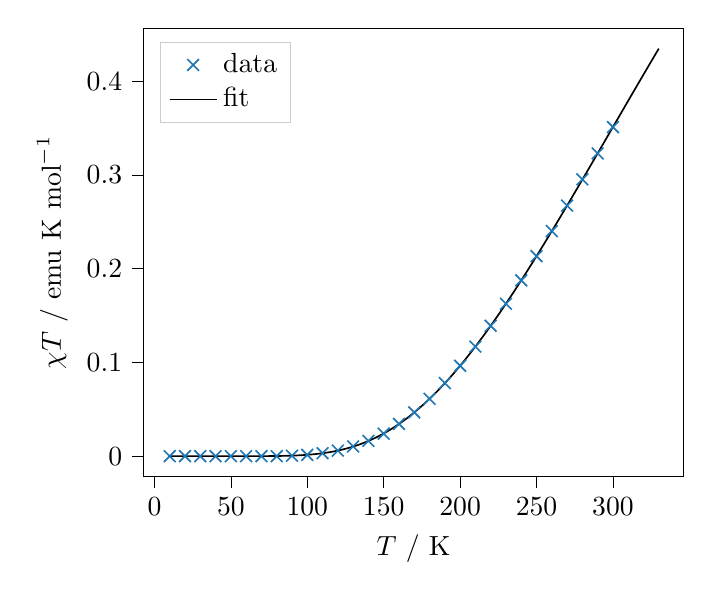
\begin{tikzpicture}

\definecolor{darkgray176}{RGB}{176,176,176}
\definecolor{lightgray204}{RGB}{204,204,204}
\definecolor{steelblue31119180}{RGB}{31,119,180}

\begin{axis}[
legend cell align={left},
legend style={
  fill opacity=0.8,
  draw opacity=1,
  text opacity=1,
  at={(0.03,0.97)},
  anchor=north west,
  draw=lightgray204
},
tick align=outside,
tick pos=left,
x grid style={darkgray176},
xlabel={\(\displaystyle T\) / \(\displaystyle \mathrm{K}\)},
xmin=-7.05, xmax=346.05,
xtick style={color=black},
y grid style={darkgray176},
ylabel={\(\displaystyle \chi T\) / \(\displaystyle \mathrm{emu\ K\ mol^{-1}}\)},
ymin=-0.0217404912428104, ymax=0.456550316099018,
ytick style={color=black}
]
\addplot [semithick, steelblue31119180, mark=x, mark size=3, mark options={solid}, only marks]
table {%
10 0
20 0
30 0
40 0
50 0
60 0
70 0
80 0
90 0.00045
100 0.00136
110 0.00317
120 0.00589
130 0.01042
140 0.01631
150 0.02401
160 0.03443
170 0.04666
180 0.06116
190 0.07792
200 0.09649
210 0.11687
220 0.13907
230 0.16263
240 0.18754
250 0.21336
260 0.24009
270 0.26727
280 0.29536
290 0.32299
300 0.35108
};
\addlegendentry{data}
\addplot [semithick, black]
table {%
9 8.38016643735043e-41
9.80451127819549 1.90995172670776e-37
10.609022556391 1.34751732815645e-34
11.4135338345865 3.77118159505316e-32
12.218045112782 5.02547307773228e-30
13.0225563909774 3.65894471249628e-28
13.8270676691729 1.61747460723547e-26
14.6315789473684 4.7137533185747e-25
15.4360902255639 9.66578332473469e-24
16.2406015037594 1.4693827393549e-22
17.0451127819549 1.7276833789531e-21
17.8496240601504 1.62671119645119e-20
18.6541353383459 1.26228411216076e-19
19.4586466165414 8.26842796459933e-19
20.2631578947368 4.66521993042709e-18
21.0676691729323 2.30637596862354e-17
21.8721804511278 1.01374762631907e-16
22.6766917293233 4.01148903190683e-16
23.4812030075188 1.44459756290231e-15
24.2857142857143 4.77883195577682e-15
25.0902255639098 1.46411970307703e-14
25.8947368421053 4.18424369757189e-14
26.6992481203008 1.1224686306635e-13
27.5037593984962 2.84223534617122e-13
28.3082706766917 6.82671863737044e-13
29.1127819548872 1.56218117110539e-12
29.9172932330827 3.41912511849611e-12
30.7218045112782 7.18260239789472e-12
31.5263157894737 1.45276671124663e-11
32.3308270676692 2.83717009562223e-11
33.1353383458647 5.36363534721082e-11
33.9398496240602 9.83832767404891e-11
34.7443609022556 1.75461690738482e-10
35.5488721804511 3.04839115583748e-10
36.3533834586466 5.16822571140266e-10
37.1578947368421 8.56415064481115e-10
37.9624060150376 1.3890899173454e-09
38.7669172932331 2.20830191593646e-09
39.5714285714286 3.44508779235659e-09
40.3759398496241 5.28013756681534e-09
41.1804511278196 7.95874127304325e-09
41.984962406015 1.18090312008327e-08
42.7894736842105 1.72639468962189e-08
43.593984962406 2.4887347923067e-08
44.3984962406015 3.5404687290838e-08
45.203007518797 4.97386363092744e-08
46.0075187969925 6.90500195940958e-08
46.812030075188 9.47843774893778e-08
47.6165413533835 1.28724423051343e-07
48.4210526315789 1.73048602962165e-07
49.2255639097744 2.30395907518825e-07
50.0300751879699 3.03937005527949e-07
50.8345864661654 3.97451706985559e-07
51.6390977443609 5.15412681328551e-07
52.4436090225564 6.63075283306003e-07
53.2481203007519 8.46573263580393e-07
54.0526315789474 1.07302006839413e-06
54.8571428571429 1.35061536327345e-06
55.6616541353383 1.68875635089926e-06
56.4661654135338 2.09815339390676e-06
57.2706766917293 2.59094940027112e-06
58.0751879699248 3.18084238271233e-06
58.8796992481203 3.88321056465794e-06
59.6842105263158 4.71523937402047e-06
60.4887218045113 5.69604964250746e-06
61.2932330827068 6.84682631236985e-06
62.0977443609023 8.19094694426721e-06
62.9022556390977 9.75410931902614e-06
63.7067669172932 1.15644574321382e-05
64.5112781954887 1.36527051924466e-05
65.3157894736842 1.60522571551083e-05
66.1203007518797 1.87993256430353e-05
66.9248120300752 2.19330436400381e-05
67.7293233082707 2.54955728721927e-05
68.5338345864662 2.95322065309438e-05
69.3383458646616 3.40914661314905e-05
70.1428571428571 3.92251920425121e-05
70.9473684210526 4.49886272676745e-05
71.7518796992481 5.14404941050671e-05
72.5563909774436 5.86430633572338e-05
73.3609022556391 6.66622158112886e-05
74.1654135338346 7.55674957553016e-05
74.9699248120301 8.54321563432964e-05
75.7744360902256 9.63331966664492e-05
76.5789473684211 0.000108351390432105
77.3834586466165 0.000121571306194738
78.187969924812 0.000136081319123754
78.9924812030075 0.000151973614331834
79.796992481203 0.000169344181824252
80.6015037593985 0.000188292803164017
81.406015037594 0.000208923029979861
82.2105263157895 0.00023134215447379
83.015037593985 0.0002556611721122
83.8195488721804 0.000281994736709424
84.6240601503759 0.000310461108134927
85.4285714285714 0.000341182092895397
86.2330827067669 0.000374282977860556
87.0375939849624 0.000409892457416896
87.8421052631579 0.000448142554346566
88.6466165413534 0.000489168534739689
89.4511278195489 0.000533108817257212
90.2556390977444 0.000580104877068427
91.0601503759399 0.000630301144792434
91.8646616541353 0.000683844900776172
92.6691729323308 0.000740886165043522
93.4736842105263 0.000801577583250202
94.2781954887218 0.000866074308978126
95.0827067669173 0.000934533882700525
95.8872180451128 0.00100711610774555
96.6917293233083 0.00108398292358152
97.4962406015038 0.0011652982767414
98.3007518796992 0.00125122798969771
99.1052631578947 0.00134193962799182
99.9097744360902 0.00143760236591388
100.714285714286 0.00153838685102112
101.518796992481 0.00164446506777327
102.323308270677 0.00175601020055489
103.127819548872 0.00187319649634407
103.932330827068 0.00199619912727781
104.736842105263 0.00212519405335348
105.541353383459 0.00226035788549604
106.345864661654 0.00240186774920984
107.15037593985 0.00254990114902365
107.954887218045 0.00270463583392704
108.759398496241 0.00286624966398553
109.563909774436 0.00303492047831217
110.368421052632 0.0032108259645622
111.172932330827 0.003394143530108
111.977443609023 0.00358505017504114
112.781954887218 0.00378372236713893
113.586466165414 0.00399033591892289
114.390977443609 0.00420506586692779
115.195488721805 0.00442808635329022
116 0.00465957050975738
116.804511278195 0.00489969034420775
117.609022556391 0.00514861662976734
118.413533834586 0.00540651879659697
119.218045112782 0.00567356482641848
120.022556390977 0.00594992114984011
120.827067669173 0.00623575254653435
121.631578947368 0.00653122204831449
122.436090225564 0.00683649084514964
123.240601503759 0.00715171819415162
124.045112781955 0.0074770613315611
124.84962406015 0.00781267538775463
125.654135338346 0.00815871330528879
126.458646616541 0.00851532575999231
127.263157894737 0.00888266108511235
128.067669172932 0.00926086519851608
128.872180451128 0.00965008153294478
129.676691729323 0.0100504509693127
130.481203007519 0.0104621117730402
131.285714285714 0.0108851995334052
132.09022556391 0.0113198471058959
132.894736842105 0.0117661845575417
133.699248120301 0.012224339115198
134.503759398496 0.0126944351167583
135.308270676692 0.0131765939652613
136.112781954887 0.0136709340858621
136.917293233083 0.0141775708856309
137.721804511278 0.0146966167161437
138.526315789474 0.0152281808388238
139.330827067669 0.0157723693929945
140.135338345865 0.0163292853666006
140.93984962406 0.0168990285695528
141.744360902256 0.0174816956096514
142.548872180451 0.018077379871042
143.353383458647 0.0186861714951542
144.157894736842 0.0193081573640764
144.962406015038 0.0199434210863152
145.766917293233 0.02059204298489
146.571428571429 0.0212541000877116
147.375939849624 0.021929666120192
148.18045112782 0.0226188115000348
148.984962406015 0.023321603334153
149.789473684211 0.02403810541766
150.593984962406 0.0247683782348835
151.398496240602 0.0255124789623465
152.203007518797 0.0262704614736636
153.007518796992 0.0270423763462985
153.812030075188 0.0278282708701302
154.616541353383 0.0286281890577742
155.421052631579 0.0294421716566058
156.225563909774 0.0302702561624332
157.03007518797 0.0311124768347675
157.834586466165 0.031968864713638
158.639097744361 0.0328394476378998
159.443609022556 0.0337242502649844
160.248120300752 0.0346232940920404
161.052631578947 0.0355365974784147
161.857142857143 0.036464175669425
162.661654135338 0.0374060408213726
163.466165413534 0.0383622020277476
164.270676691729 0.0393326653465789
165.075187969925 0.0403174338288798
165.87969924812 0.0413165075481435
166.684210526316 0.0423298836308421
167.488721804511 0.0433575562878825
168.293233082707 0.0443995168469752
169.097744360902 0.0454557537858714
169.902255639098 0.0465262527664253
170.706766917293 0.0476109966694374
171.511278195489 0.0487099656302395
172.315789473684 0.0498231370749768
173.12030075188 0.0509504857575491
173.924812030075 0.0520919837971703
174.729323308271 0.0532476007165076
175.533834586466 0.0544173034803614
176.338345864662 0.0556010565348504
177.142857142857 0.0567988218470621
177.947368421053 0.0580105589451371
178.751879699248 0.0592362249587476
179.556390977444 0.0604757746599401
180.360902255639 0.0617291605043055
181.165413533835 0.0629963326724462
181.96992481203 0.0642772391117068
182.774436090226 0.0655718255781389
183.578947368421 0.0668800356786678
184.383458646617 0.0682018109134335
185.187969924812 0.069537090718276
185.992481203008 0.0708858125073372
186.796992481203 0.0722479117157526
187.601503759398 0.073623321842406
188.406015037594 0.0750119744927216
189.210526315789 0.0764137994214689
190.015037593985 0.0778287245755552
190.81954887218 0.0792566761367843
191.624060150376 0.0806975785645556
192.428571428571 0.0821513546384849
193.233082706767 0.0836179255009234
194.037593984962 0.085097210699355
194.842105263158 0.0865891282286518
195.646616541353 0.0880935945731696
196.451127819549 0.0896105247486631
197.255639097744 0.0911398323440046
198.06015037594 0.0926814295626875
198.864661654135 0.0942352272641003
199.669172932331 0.0958011350045518
200.473684210526 0.0973790610780359
201.278195488722 0.0989689125567185
202.082706766917 0.100570595331134
202.887218045113 0.102184014150076
203.691729323308 0.103809072660176
204.496240601504 0.105445673445142
205.300751879699 0.10709371806467
206.105263157895 0.108753107092989
206.90977443609 0.110423740157054
207.714285714286 0.11210551597436
208.518796992481 0.113798332390372
209.323308270677 0.115502086415569
210.127819548872 0.117216674262084
210.932330827068 0.118941991379935
211.736842105263 0.120677932492841
212.541353383459 0.122424391633613
213.345864661654 0.124181262179124
214.15037593985 0.125948436884825
214.954887218045 0.127725807918842
215.759398496241 0.129513266895605
216.563909774436 0.131310704909038
217.368421052632 0.133118012565289
218.172932330827 0.134935080014999
218.977443609023 0.136761796985105
219.781954887218 0.138598052810178
220.586466165414 0.140443736463286
221.390977443609 0.142298736586394
222.195488721805 0.144162941520273
223 0.146036239333943
223.804511278195 0.147918517853634
224.609022556391 0.149809664691263
225.413533834586 0.151709567272433
226.218045112782 0.153618112863951
227.022556390977 0.155535188600858
227.827067669173 0.15746068151298
228.631578947368 0.159394478550996
229.436090225564 0.161336466612024
230.240601503759 0.163286532564721
231.045112781955 0.165244563273912
231.84962406015 0.167210445624728
232.654135338346 0.169184066546272
233.458646616541 0.17116531303481
234.263157894737 0.17315407217648
235.067669172932 0.175150231169537
235.872180451128 0.17715367734612
236.676691729323 0.179164298193552
237.481203007519 0.18118198137518
238.285714285714 0.183206614750744
239.09022556391 0.185238086396289
239.894736842105 0.187276284623621
240.699248120301 0.189321097999309
241.503759398496 0.191372415363235
242.308270676692 0.193430125846695
243.112781954887 0.19549411889006
243.917293233083 0.197564284259997
244.721804511278 0.199640512066254
245.526315789474 0.201722692778006
246.330827067669 0.203810717239784
247.135338345865 0.205904476686975
247.93984962406 0.208003862760897
248.744360902256 0.210108767523473
249.548872180451 0.212219083471477
250.353383458647 0.214334703550387
251.157894736842 0.216455521167829
251.962406015038 0.218581430206628
252.766917293233 0.220712325037465
253.571428571429 0.222848100531145
254.375939849624 0.224988652070482
255.18045112782 0.227133875561814
255.984962406015 0.229283667446131
256.789473684211 0.231437924709846
257.593984962406 0.233596544895201
258.398496240602 0.235759426110308
259.203007518797 0.237926467038849
260.007518796992 0.240097566949416
260.812030075188 0.242272625704514
261.616541353383 0.244451543769227
262.421052631579 0.246634222219549
263.225563909774 0.248820562750388
264.03007518797 0.251010467683248
264.834586466165 0.25320383997359
265.639097744361 0.25540058321789
266.443609022556 0.257600601660379
267.248120300752 0.259803800199488
268.052631578947 0.262010084393991
268.857142857143 0.264219360468865
269.661654135338 0.266431535320851
270.466165413534 0.268646516523746
271.270676691729 0.270864212333406
272.075187969925 0.273084531692488
272.87969924812 0.275307384234922
273.684210526316 0.277532680290116
274.488721804511 0.279760330886913
275.293233082707 0.28199024775729
276.097744360902 0.284222343339815
276.902255639098 0.286456530782857
277.706766917293 0.288692723947564
278.511278195489 0.290930837410604
279.315789473684 0.293170786466681
280.12030075188 0.295412487130832
280.924812030075 0.297655856140495
281.729323308271 0.299900810957377
282.533834586466 0.302147269769101
283.338345864662 0.304395151490659
284.142857142857 0.306644375765658
284.947368421053 0.308894862967372
285.751879699248 0.311146534199608
286.556390977444 0.313399311297378
287.360902255639 0.315653116827396
288.165413533835 0.317907874088389
288.96992481203 0.320163507111245
289.774436090226 0.322419940658982
290.578947368421 0.324677100226556
291.383458646617 0.326934912040508
292.187969924812 0.329193303058451
292.992481203008 0.331452200968409
293.796992481203 0.333711534188002
294.601503759398 0.335971231863484
295.406015037594 0.33823122386865
296.210526315789 0.340491440803591
297.015037593985 0.342751813993325
297.81954887218 0.345012275486295
298.624060150376 0.347272758052739
299.428571428571 0.349533195182938
300.233082706767 0.351793521085344
301.037593984962 0.354053670684592
301.842105263158 0.356313579619399
302.646616541353 0.358573184240354
303.451127819549 0.360832421607604
304.255639097744 0.363091229488431
305.06015037594 0.365349546354735
305.864661654135 0.367607311380421
306.669172932331 0.369864464438688
307.473684210526 0.372120946099229
308.278195488722 0.374376697625349
309.082706766917 0.376631660970993
309.887218045113 0.37888577877769
310.691729323308 0.381138994371428
311.496240601504 0.383391251759445
312.300751879699 0.385642495626949
313.105263157895 0.387892671333766
313.90977443609 0.390141724910929
314.714285714286 0.392389603057186
315.518796992481 0.39463625313546
316.323308270677 0.396881623169242
317.127819548872 0.399125661838926
317.932330827068 0.401368318478091
318.736842105263 0.403609543069729
319.541353383459 0.405849286242421
320.345864661654 0.408087499266468
321.15037593985 0.410324134049971
321.954887218045 0.412559143134874
322.759398496241 0.414792479692955
323.563909774436 0.417024097521786
324.368421052632 0.419253951040652
325.172932330827 0.421481995286434
325.977443609023 0.423708185909456
326.781954887218 0.425932479169307
327.586466165414 0.428154831930623
328.390977443609 0.430375201658847
329.195488721805 0.432593546415965
330 0.434809824856208
};
\addlegendentry{fit}
\end{axis}

\end{tikzpicture}

            \caption{The measured and fitted \(\chi T\) against \(T\) for the \(\mathrm{Cu_{2}}\) cluster.}
            \label{Fig:Cu2cluster}
        \end{figure}
    \end{ex}

    \subsection{Modelling Exchange Interactions in Clusters}
    Now let's see how do we solve for the exact magnetic energy levels and \(\chi T(T)\) expressions for simple systems. The recipe is as follows:
    \begin{enumerate}
        \item Set up the Hamiltonian. The \textit{Heisenberg--Dirac--van Vleck Hamiltonian} is\footnote{Here we assumed both the spins and the interactions are \textit{isotropic}, i.e. the same in every direction. We will explore more possibility later.}
        \begin{equation}
            \hat{H}=-2\sum_{i>j}J_{ij}\hat{\vb{S}}_i\hat{\vb{S}}_j\,,
        \end{equation}
        where \(\hat{\vb{S}}_i\) is the spin operator for particle \(i\), and \(J_{ij}\) is the coupling strength between spin \(i\) and spin \(j\): it's positive for ferromagnetic coupling and negative for antiferromagnetic coupling.

        Practically, we don't need to couple all pairs of atoms in a cluster: we only need to consider the coupling between two spin carriers if they are close enough for the interaction to be significant. This means that we can set \(J_{ij}=0\) if \(i\) and \(j\) are far enough. Moreover, some \(J\) values may be identical by symmetry, which further simplifies the expression of the Hamiltonian. A few examples of spin Hamiltonians for simple systems are given in \cref{Fig:Hamiltonians} --- we will not consider any system more complex than these in this course.

        \begin{figure}[ht!]
            \centering
            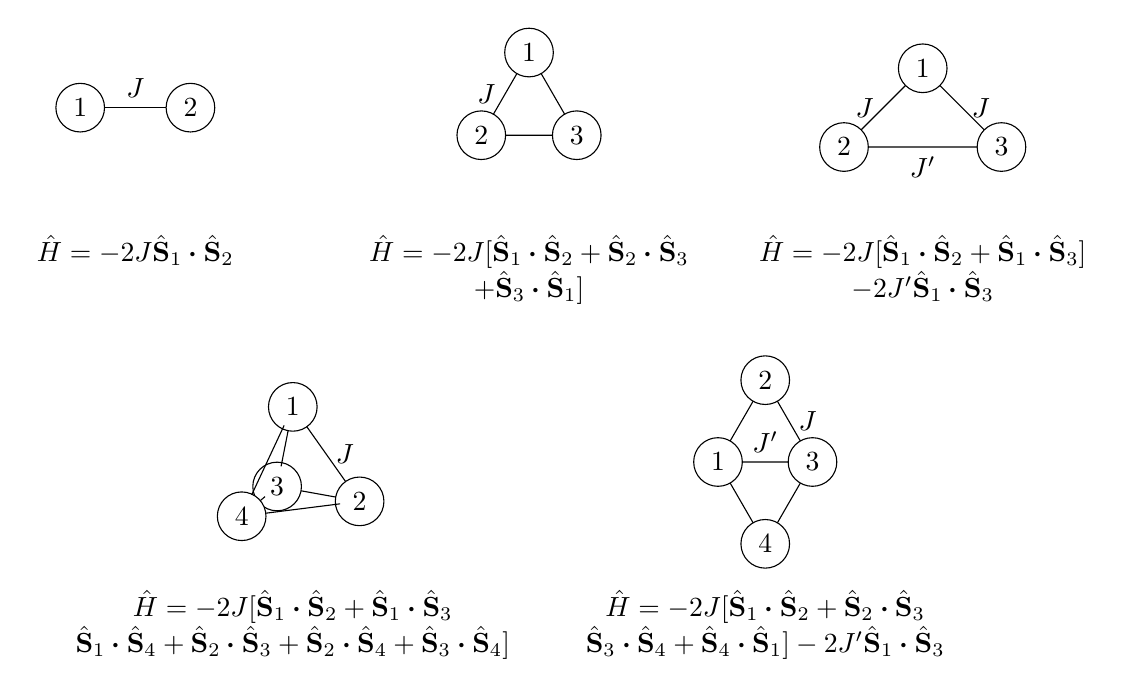
\begin{tikzpicture}
                \draw (-0.7,0)node[circle, draw, fill=white]{\(1\)}--node[above]{\(J\)}(0.7,0)node[circle, draw, fill=white]{\(2\)};
                \node at (0,-1.5) [below] {\(\hat{H}=-2J\hat{\vb{S}}_1\vdot\hat{\vb{S}}_2\)};

                \begin{scope}[shift={(5,0)}]
                    \draw (90:0.7)node[circle, draw, fill=white]{\(1\)} --node[left]{\(J\)} (210:0.7)node[circle, draw, fill=white]{\(2\)} -- (-30:0.7)node[circle, draw, fill=white]{\(3\)} -- cycle;
                    \node at (0,-1.5) [below, align=center] {\(\hat{H}=-2J[\hat{\vb{S}}_1\vdot\hat{\vb{S}}_2+\hat{\vb{S}}_2\vdot\hat{\vb{S}}_3\) \\ \(+\hat{\vb{S}}_3\vdot\hat{\vb{S}}_1]\)};
                \end{scope}

                \begin{scope}[shift={(10,0)}]
                    \draw (0,0.5)node[circle, draw, fill=white]{\(1\)} --node[left]{\(J\)} (-1,-0.5)node[circle, draw, fill=white]{\(2\)} --node[below]{\(J'\)} (1, -0.5) node[circle, draw, fill=white]{\(3\)} --node[right]{\(J\)} cycle;
                    \node at (0,-1.5) [below, align=center] {\(\hat{H}=-2J[\hat{\vb{S}}_1\vdot\hat{\vb{S}}_2+\hat{\vb{S}}_1\vdot\hat{\vb{S}}_3]\) \\ \(-2J'\hat{\vb{S}}_1\vdot\hat{\vb{S}}_3\)};
                \end{scope}

                \begin{scope}[shift={(2,-4.5)}, z={(40:0.4)}]
                    \coordinate (A) at (0,0.7,0);
                    \coordinate (B) at ({0.8485 * cos(0)},-0.5,{0.8485 * sin(0)});
                    \coordinate (C) at ({0.8485 * cos(120)},-0.5,{0.8485 * sin(120)});
                    \coordinate (D) at ({0.8485 * cos(240)},-0.5,{0.8485 * sin(240)});

                    \draw (A)node[circle, draw, fill=white]{\(1\)}--node[right]{\(J\)}(B)node[circle, draw, fill=white]{\(2\)}--(C)node[circle, draw, fill=white]{\(3\)}--(D)node[circle, draw, fill=white]{\(4\)};
                    \draw[shorten <= 0.3cm, shorten >= 0.25cm] (D)--(B);
                    \draw[shorten <= 0.3cm, shorten >= 0.26cm] (A)--(C);
                    \draw[shorten <= 0.26cm, shorten >= 0.3cm] (A)--(D);
                    \draw[shorten <= 0.2cm, shorten >= 0.31cm] (C)--(D);
                    \node at (0,-1.5) [below, align=center] {\(\hat{H}=-2J[\hat{\vb{S}}_1\vdot\hat{\vb{S}}_2+\hat{\vb{S}}_1\vdot\hat{\vb{S}}_3\) \\ \(\hat{\vb{S}}_1\vdot\hat{\vb{S}}_4+\hat{\vb{S}}_2\vdot\hat{\vb{S}}_3+\hat{\vb{S}}_2\vdot\hat{\vb{S}}_4+\hat{\vb{S}}_3\vdot\hat{\vb{S}}_4]\)};
                \end{scope}
                \begin{scope}[shift={(8,-4.5)}]
                    \coordinate (A) at (-0.6,0);
                    \coordinate (B) at (0.6,0);
                    \coordinate (C) at (0,1.0392);
                    \coordinate (D) at (0,-1.0392);
                    \draw (A) --node[above]{\(J'\)} (B) --node[right]{\(J\)} (C) node[circle, draw, fill=white]{\(2\)} -- (A)node[circle, draw, fill=white]{\(1\)} -- (D) node[circle, draw, fill=white]{\(4\)} -- (B)node[circle, draw, fill=white]{\(3\)};
                    \node at (0,-1.5) [below, align=center] {\(\hat{H}=-2J[\hat{\vb{S}}_1\vdot\hat{\vb{S}}_2+\hat{\vb{S}}_2\vdot\hat{\vb{S}}_3\) \\ \(\hat{\vb{S}}_3\vdot\hat{\vb{S}}_4+\hat{\vb{S}}_4\vdot\hat{\vb{S}}_1]-2J'\hat{\vb{S}}_1\vdot\hat{\vb{S}}_3\)};
                \end{scope}
            \end{tikzpicture}
            \caption{Examples of spin Hamiltonians of small clusters.}
            \label{Fig:Hamiltonians}
        \end{figure}

        \item Solving the spin Hamiltonian. This is the hard bit. The brute force approach is matrix diagonalisation. This is discussed in appendix \cref{Chap:Spin_matrix}, assuming familiarity with quantum mechanics.
        
        Here we will instead use another method called \textit{Kambe vector coupling}. It does not involve diagonalising a matrix, and easily doable by hand for small systems. The basic idea of this method is that although we don't know the eigenvalues of \(\hat{\vb{S}}_1\vdot\hat{\vb{S}}_2\) of two spins, we do know that of \((\hat{\vb{S}}_1+\hat{\vb{S}}_2)^2\equiv \hat{\vb{S}}_{\text{T}}^2\): if spin 1 has spin quantum number \(S_1\) and spin 2 has spin quantum number \(S_2\), then the total spin can take is quantum number \(S_{\text{T}}\) in \(S_1+S_2, S_1+S_2-1,\dots\abs{S_1-S_2}\). Moreover, since
        \begin{equation}
            \hat{\vb{S}}_{\text{T}}^2=(\hat{\vb{S}}_1+\hat{\vb{S}}_2)^2=\hat{\vb{S}}_1^2+\hat{\vb{S}}_2^2+2\hat{\vb{S}}_1\vdot\hat{\vb{S}}_2\,,
        \end{equation}
        we can rewrite the coupling Hamiltonian as
        \begin{equation}
            \hat{H}_{ij}=-2J\vb{S}_1\vdot\vb{S}_2=J[\hat{\vb{S}}_1^2+\hat{\vb{S}}_2^2-\hat{\vb{S}}_{\text{T}}^2]\,.
        \end{equation}
        Since the eigenvalue of the squared (spin) angular momentum operator is \(\hat{\vb{S}}^2\ket{S}=S(S+1)\ket{S}\), the energy spectrum of \(\hat{H}_{ij}\) is therefore
        \begin{equation}
            E(S_{\text{T}}, S_1, S_2)=J[S_1(S_1+1) + S_2(S_2+1) - S_{\text{T}}(S_{\text{T}}+1)]\,.
        \end{equation}

        The above process solves the coupling between two spins. It can be generalised to the coupling between more spins --- although it gets algebraically tricker, it is still essentially just rewriting the dot product of spin operators in terms of the squared spin operators. We will see a couple of examples later.

        \item Finally, to work out the magnetic susceptibility at a certain temperature, we need to apply the Boltzmann distribution to work out the thermal average.
        
        A state with total spin \(S_{\text{T}}\) has magnetic susceptibility
        \begin{equation}
            \chi(S_{\text{T}})=\frac{N_Ag^2\mu_{\text{B}}^2}{3k_B T}S_{\text{T}}(S_{\text{T}}+1)\,.
        \end{equation}
        Suppose it has energy \(E(S_{\text{T}})\), since the degeneracy of the state is \(2S_{\text{T}}+1\), it carries Boltzmann weight
        \begin{equation}
            (2S_{\text{T}}+1)e^{-E(S_{\text{T}})/k_B T}\,.
        \end{equation}
        The thermal (canonical) average of the magnetic susceptibility is therefore
        \begin{equation}
            \chi=\frac{N_Ag^2\mu_{\text{B}}^2}{3k_B T}\frac{\sum_{S_{\text{T}}} S_{\text{T}}(S_{\text{T}}+1) (2S_{\text{T}}+1)e^{-E(S_{\text{T}})/k_B T}}{\sum_{S_{\text{T}}}(2S_{\text{T}}+1)e^{-E(S_{\text{T}})/k_B T}}\,.
        \end{equation}
        This is the \textit{van Vleck equation}.

    \end{enumerate}

    Let's see a couple of examples.

    \begin{ex}
        \textit{A \(\mathrm{Cu(II)/Mn(II)}\) dimer.}

        Let's have a look at the \(\mathrm{Cu(II)/Mn(II)}\) complex \(\mathrm{Cu[(prp)_2pr]Mn(hfac)_2}\) was reported by Brewer and Sinn (\textit{Inorg.Chem}, 1987, 26, 1529). It was studied as part of a more extended study of heteronuclear diatomics as models for the enzyme cytochrome oxidase. The structure of the \(\mathrm{Fe}\) analogue is shown below. The two metal ions are bridged by two \(\mu_2\)-phenoxy groups which are likely to provide the superexchange pathway.

        \begin{figure}[ht!]
            \centering
            \begin{tikzpicture}
                \node at (0,0){\includesvg[width=0.45\textwidth]{figures/Cu_Mn_dimer}};
                \draw[red,dashed,thick] (-3.5,-2.8) rectangle (-1.55,0.9);
                \draw[blue,dashed,thick] (-0.45,-3.1) rectangle (1.35,-0.6);
                \node[red] at (-4.8,-0.5){
                    \chemfig{[:150]Fe**[60,300,dash pattern=on 3pt off 3pt]6(-O-(-CF_3)--(-CF_3)-O-)}
                    \chemmove{
                        \node[at=(cyclecenter1)](){\(\ominus\)};
                    }
                };
                \node[blue] at (4.8,-0.5){
                    \definesubmol{wb}{
                        (-[::90,.5,,,draw=none]%
                        -[::180,,,,blue,decorate,decoration={%
                        snake,amplitude=0.2mm,segment length=0.75mm }%
                    ])}
                    \chemfig{*6(-=-(-!{wb})=(-O(-[:30]Cu)-[:150]Fe)-=)}
                };
            \end{tikzpicture}
            \caption{X-ray structure of the \(\mathrm{Fe}\) analogue \(\mathrm{Cu[(prp)_2pr]Fe(hfac)_2}\).}
        \end{figure}

        The compound has spin Hamiltonian
        \begin{equation}
            \hat{H}=-2J\hat{\vb{S}}_{\mathrm{Cu}}\vdot\hat{\vb{S}}_{\mathrm{Mn}}\,.
        \end{equation}
        \(\mathrm{Cu^{II}}\) and \(\mathrm{Mn^{II}}\) have spins \(S_{\mathrm{Cu}}=\frac{1}{2}\) and \(S_{\mathrm{Mn}}=\frac{5}{2}\) respectively. When the two ions couple, the total spin \(S_{\text{T}}\) takes values \(S_{\text{T}}\in\{S_{\mathrm{Cu}}+S_{\mathrm{Mn}}, \dots, \abs{S_{\mathrm{Cu}}-S_{\mathrm{Mn}}}\}=\{3,2\}\).

        Using the Kambe vector coupling method, the spin Hamiltonian can be rewritten as
        \begin{equation}
            \hat{H}=J[\hat{\vb{S}}_{\mathrm{Cu}}^2+\hat{\vb{S}}_{\mathrm{Mn}}^2-\hat{\vb{S}}_{\text{T}}^2]\,,
        \end{equation}
        and so the energy spectrum are
        \begin{align}
            E&=J[S_{\mathrm{Cu}}(S_{\mathrm{Cu}}+1)+S_{\mathrm{Mn}}(S_{\mathrm{Mn}})-S_{\text{T}}(S_{\text{T}}+1)] \notag \\
            &=J\left[\frac{19}{2}-S_{\text{T}}(S_{\text{T}}+1)\right]\,.
        \end{align}

        The energy eigenvalues are tabulated as follows.

        \begin{table}[ht!]
            \renewcommand{\arraystretch}{1.2}
            \centering
            \begin{tabular}{cccc}
                \toprule
                \(S_{\mathrm{Cu}}\) & \(S_{\mathrm{Mn}}\) & \(S_{\text{T}}\) & \(E\) \\ \midrule
                \(\frac{1}{2}\) & \(\frac{5}{2}\) & \(3\) & \(-\frac{5}{2}J\) \\
                \(\frac{1}{2}\) & \(\frac{5}{2}\) & \(2\) & \(+\frac{7}{2}J\) \\ \bottomrule
            \end{tabular}
        \end{table}

        A convenient sanity check of the solutions obtained is that the `centre of mass' of these energy levels, accounting for the degeneracies, should be zero:
        \begin{equation}
            \sum E(S_{\text{T}}) (2S_{\text{T}}+1)=0\,.
        \end{equation}
        Now, applying the van Vleck equation, we get the temperature-dependent magnetic susceptibility
        \begin{equation}
            \chi=\frac{N_Ag^2\mu_{\text{B}}^2}{3k_B T}\frac{84\ee^{6J/k_B T}+30}{7\ee^{6J/k_B T}+5}\,.
        \end{equation}

        The experimental \(\chi T\) value of this compound is shown in \cref{Fig:Cu_Mn_cluster}. Our theoretical model fits the data really well, giving \(J/k_B=-21\unit{K}\) and \(g=2.05\). The coupling is antiferromagnetic.

        We can also double check the high temperature and low temperature limit. When \(T\to 0\), only the \(S_{\text{T}}=2\) ground state is occupied, giving
        \begin{equation}
            \lim_{T\to 0}\chi T =\frac{1}{8}g^2S_{\text{T}}(S_{\text{T}}+1)\approx 3.15\unit{emu}\unit{K}\unit{mol}^{-1}
        \end{equation}
        using the fitted \(g\) value of \(2.05\). (An \textit{a priori} estimation using \(g\approx 2.0\) would give \(\chi T\to 3.0\unit{emu}\unit{K}\unit{mol}^{-1}\).) The high temperature limit is
        \begin{equation}
            \lim_{T\to\infty}\chi T=\frac{1}{8}g^2\sum_i S_i(S_i+1)=4.99\unit{emu}\unit{K}\unit{mol}^{-1}
        \end{equation}
        using \(g\approx 2.05\) (\(g=2.0\) gives \(\chi T\to 3.75\unit{emu}\unit{K}\unit{mol}^{-1}\)). We see that our graph hasn't reached this limit yet.

        \begin{figure}
            \centering
            % This file was created with matplot2tikz v0.4.0.
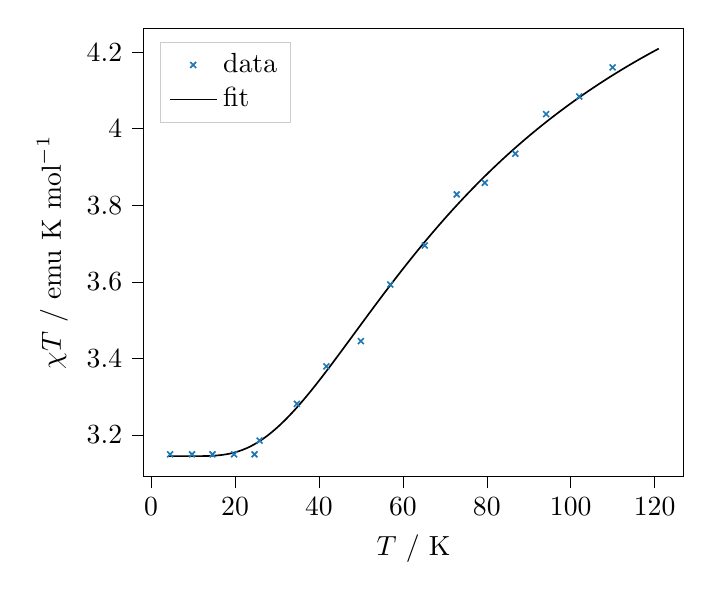
\begin{tikzpicture}

\definecolor{darkgray176}{RGB}{176,176,176}
\definecolor{lightgray204}{RGB}{204,204,204}
\definecolor{steelblue31119180}{RGB}{31,119,180}

\begin{axis}[
legend cell align={left},
legend style={
  fill opacity=0.8,
  draw opacity=1,
  text opacity=1,
  at={(0.03,0.97)},
  anchor=north west,
  draw=lightgray204
},
tick align=outside,
tick pos=left,
x grid style={darkgray176},
xlabel={\(\displaystyle T\) / \(\displaystyle \mathrm{K}\)},
xmin=-1.76233605, xmax=126.82938105,
xtick style={color=black},
y grid style={darkgray176},
ylabel={\(\displaystyle \chi T\) / \(\displaystyle \mathrm{emu\ K\ mol^{-1}}\)},
ymin=3.09136348821546, ymax=4.26258189296311,
ytick style={color=black}
]
\addplot [semithick, steelblue31119180, mark=x, mark size=1.5, mark options={solid}, only marks]
table {%
4.53638 3.14933
9.75749 3.14933
14.63624 3.14933
19.77176 3.14933
24.6505 3.14933
25.84879 3.18523
34.75036 3.28144
41.7689 3.37908
49.98574 3.44513
57.00428 3.59303
65.22112 3.69497
72.8388 3.82851
79.51499 3.85867
86.7903 3.93477
94.15122 4.03815
102.02568 4.0841
109.98573 4.16021
};
\addlegendentry{data}
\addplot [semithick, black]
table {%
4.082742 3.14460068843126
4.37572836842105 3.14460068843443
4.66871473684211 3.14460068845173
4.96170110526316 3.14460068852851
5.25468747368421 3.14460068881456
5.54767384210526 3.14460068973506
5.84066021052632 3.1446006923513
6.13364657894737 3.14460069903927
6.42663294736842 3.1446007146455
6.71961931578947 3.1446007482961
7.01260568421053 3.1446008160271
7.30559205263158 3.14460094437145
7.59857842105263 3.14460117498153
7.89156478947369 3.14460157029391
8.18455115789474 3.144602220164
8.47753752631579 3.14460324932204
8.77052389473684 3.14460482543701
9.0635102631579 3.14460716752703
9.35649663157895 3.14461055442697
9.649483 3.14461533301649
9.94246936842105 3.14462192592311
10.2354557368421 3.14463083844163
10.5284421052632 3.14464266444982
10.8214284736842 3.14465809114632
11.1144148421053 3.14467790248626
11.4074012105263 3.14470298123989
11.7003875789474 3.14473430964701
11.9933739473684 3.14477296868268
12.2863603157895 3.14482013598681
12.5793466842105 3.144877082541
12.8723330526316 3.14494516819941
13.1653194210526 3.14502583619849
13.4583057894737 3.14512060678104
13.7512921578947 3.14523107007652
14.0442785263158 3.14535887838061
14.3372648947368 3.14550573797439
14.6302512631579 3.14567340061804
14.9232376315789 3.14586365484564
15.216224 3.14607831717816
15.5092103684211 3.14631922336075
15.8021967368421 3.14658821971879
16.0951831052632 3.1468871547158
16.3881694736842 3.14721787078407
16.6811558421053 3.14758219648828
16.9741422105263 3.14798193907112
17.2671285789474 3.14841887742023
17.5601149473684 3.14889475548627
17.8531013157895 3.14941127617388
18.1460876842105 3.14997009571931
18.4390740526316 3.1505728185622
18.7320604210526 3.15122099271287
19.0250467894737 3.15191610561143
19.3180331578947 3.15265958047089
19.6110195263158 3.15345277309242
19.9040058947368 3.15429696913832
20.1969922631579 3.15519338184539
20.4899786315789 3.15614315015996
20.782965 3.1571473372738
21.0759513684211 3.15820692953957
21.3689377368421 3.15932283574353
21.6619241052632 3.16049588671275
21.9549104736842 3.16172683523422
22.2478968421053 3.16301635626299
22.5408832105263 3.16436504739715
22.8338695789474 3.16577342959754
23.1268559473684 3.16724194813086
23.4198423157895 3.16877097371556
23.7128286842105 3.17036080385044
24.0058150526316 3.17201166430696
24.2988014210526 3.17372371076695
24.5917877894737 3.17549703058841
24.8847741578947 3.17733164468288
25.1777605263158 3.17922750948907
25.4707468947368 3.18118451902793
25.7637332631579 3.18320250702563
26.056719631579 3.18528124909171
26.349706 3.18742046494042
26.6426923684211 3.18961982064426
26.9356787368421 3.19187893090953
27.2286651052632 3.19419736136444
27.5216514736842 3.19657463085125
27.8146378421053 3.19901021371433
28.1076242105263 3.20150354207716
28.4006105789474 3.20405400810158
28.6935969473684 3.20666096622342
28.9865833157895 3.20932373535914
29.2795696842105 3.21204160107889
29.5725560526316 3.2148138177415
29.8655424210526 3.21763961058793
30.1585287894737 3.22051817778971
30.4515151578947 3.22344869244969
30.7445015263158 3.22643030455254
31.0374878947368 3.22946214286307
31.3304742631579 3.23254331677058
31.623460631579 3.23567291807787
31.916447 3.23885002273389
32.2094333684211 3.24207369250918
32.5024197368421 3.24534297661351
32.7954061052632 3.2486569132555
33.0883924736842 3.25201453114397
33.3813788421053 3.25541485093125
33.6743652105263 3.25885688659862
33.9673515789474 3.26233964678423
34.2603379473684 3.26586213605429
34.5533243157895 3.26942335611788
34.8463106842105 3.27302230698649
35.1392970526316 3.27665798807894
35.4322834210526 3.28032939927289
35.7252697894737 3.28403554190375
36.0182561578947 3.28777541971236
36.3112425263158 3.29154803974247
36.6042288947368 3.29535241318928
36.8972152631579 3.29918755620041
37.190201631579 3.30305249063042
37.483188 3.30694624475042
37.7761743684211 3.31086785391396
38.0691607368421 3.31481636118067
38.3621471052632 3.31879081789888
38.6551334736842 3.32279028424884
38.9481198421053 3.32681382974757
39.2411062105263 3.33086053371707
39.5340925789474 3.33492948571693
39.8270789473684 3.3390197859429
40.1200653157895 3.34313054559267
40.4130516842105 3.34726088720011
40.7060380526316 3.35140994493936
40.9990244210526 3.35557686490002
41.2920107894737 3.35976080533462
41.5849971578947 3.36396093687961
41.8779835263158 3.36817644275113
42.1709698947368 3.37240651891667
42.4639562631579 3.37665037424365
42.756942631579 3.38090723062628
43.049929 3.38517632309148
43.3429153684211 3.38945689988516
43.6359017368421 3.39374822253962
43.9288881052632 3.39804956592338
44.2218744736842 3.40236021827395
44.5148608421053 3.40667948121494
44.8078472105263 3.41100666975801
45.1008335789474 3.41534111229071
45.3938199473684 3.41968215055104
45.6868063157895 3.42402913958943
45.9797926842105 3.42838144771897
46.2727790526316 3.43273845645463
46.5657654210526 3.4370995604422
46.8587517894737 3.44146416737752
47.1517381578947 3.44583169791678
47.4447245263158 3.45020158557849
47.7377108947369 3.45457327663766
48.0306972631579 3.45894623001281
48.323683631579 3.46331991714635
48.61667 3.46769382187887
48.9096563684211 3.47206744031783
49.2026427368421 3.47644028070107
49.4956291052632 3.48081186325575
49.7886154736842 3.48518172005296
50.0816018421053 3.48954939485857
50.3745882105263 3.49391444298061
50.6675745789474 3.49827643111359
50.9605609473684 3.50263493718019
51.2535473157895 3.50698955017049
51.5465336842105 3.51133986997918
51.8395200526316 3.51568550724109
52.1325064210526 3.52002608316511
52.4254927894737 3.5243612293671
52.7184791578947 3.52869058770171
53.0114655263158 3.53301381009355
53.3044518947369 3.53733055836795
53.5974382631579 3.54164050408132
53.890424631579 3.5459433283516
54.183411 3.5502387216887
54.4763973684211 3.55452638382536
54.7693837368421 3.55880602354834
55.0623701052632 3.56307735853038
55.3553564736842 3.56734011516278
55.6483428421053 3.57159402838896
55.9413292105263 3.57583884153901
56.2343155789474 3.58007430616537
56.5273019473684 3.58430018187975
56.8202883157895 3.5885162361914
57.1132746842105 3.59272224434677
57.4062610526316 3.59691798917075
57.6992474210526 3.60110326090942
57.9922337894737 3.60527785707453
58.2852201578947 3.60944158228962
58.5782065263158 3.61359424813801
58.8711928947369 3.61773567301252
59.1641792631579 3.62186568196719
59.457165631579 3.62598410657078
59.750152 3.63009078476235
60.0431383684211 3.63418556070873
60.3361247368421 3.63826828466409
60.6291111052632 3.64233881283145
60.9220974736842 3.64639700722636
61.2150838421053 3.65044273554257
61.5080702105263 3.65447587101982
61.8010565789474 3.65849629231376
62.0940429473684 3.66250388336789
62.3870293157895 3.66649853328771
62.6800156842105 3.67048013621691
62.9730020526316 3.67444859121572
63.2659884210526 3.67840380214131
63.5589747894737 3.68234567753035
63.8519611578947 3.68627413048363
64.1449475263158 3.69018907855278
64.4379338947369 3.69409044362906
64.7309202631579 3.6979781518342
65.023906631579 3.70185213341335
65.316893 3.70571232262992
65.6098793684211 3.70955865766265
65.9028657368421 3.71339108050446
66.1958521052632 3.71720953686344
66.4888384736842 3.72101397606572
66.7818248421053 3.7248043509603
67.0748112105263 3.72858061782583
67.3677975789474 3.73234273627919
67.6607839473684 3.7360906691861
67.9537703157895 3.73982438257343
68.2467566842105 3.7435438455434
68.5397430526316 3.74724903018963
68.8327294210526 3.75093991151484
69.1257157894737 3.75461646735046
69.4187021578947 3.75827867827785
69.7116885263158 3.76192652755126
70.0046748947369 3.76556000102246
70.2976612631579 3.76917908706705
70.590647631579 3.77278377651237
70.883634 3.77637406256699
71.1766203684211 3.77994994075178
71.4696067368421 3.78351140883258
71.7625931052632 3.7870584667543
72.0555794736842 3.79059111657661
72.3485658421053 3.794109362411
72.6415522105263 3.79761321035933
72.9345385789474 3.80110266845384
73.2275249473684 3.80457774659846
73.5205113157895 3.80803845651154
73.8134976842105 3.81148481166991
74.1064840526316 3.81491682725427
74.3994704210526 3.81833452009582
74.6924567894737 3.82173790862421
74.9854431578947 3.82512701281669
75.2784295263158 3.8285018541485
75.5714158947369 3.83186245554444
75.8644022631579 3.83520884133165
76.157388631579 3.83854103719341
76.450375 3.84185907012425
76.7433613684211 3.84516296838599
77.0363477368421 3.84845276146494
77.3293341052632 3.85172848003018
77.6223204736842 3.85499015589276
77.9153068421053 3.85823782196606
78.2082932105263 3.86147151222698
78.5012795789474 3.86469126167827
78.7942659473684 3.86789710631165
79.0872523157895 3.87108908307197
79.3802386842105 3.8742672298222
79.6732250526316 3.87743158530938
79.9662114210526 3.88058218913138
80.2591977894737 3.88371908170453
80.5521841578947 3.88684230423208
80.8451705263158 3.88995189867353
81.1381568947369 3.89304790771461
81.4311432631579 3.89613037473819
81.724129631579 3.8991993437959
82.017116 3.90225485958041
82.3101023684211 3.90529696739859
82.6030887368421 3.90832571314524
82.8960751052632 3.91134114327758
83.1890614736842 3.91434330479042
83.4820478421053 3.91733224519198
83.7750342105263 3.92030801248032
84.0680205789474 3.9232706551205
84.3610069473684 3.92622022202223
84.6539933157895 3.92915676251822
84.9469796842105 3.93208032634308
85.2399660526316 3.93499096361281
85.5329524210526 3.93788872480482
85.8259387894737 3.94077366073853
86.1189251578948 3.94364582255652
86.4119115263158 3.94650526170611
86.7048978947369 3.94935202992162
86.9978842631579 3.95218617920692
87.290870631579 3.95500776181865
87.583857 3.9578168302498
87.8768433684211 3.96061343721379
88.1698297368421 3.96339763562901
88.4628161052632 3.96616947860381
88.7558024736842 3.96892901942185
89.0487888421053 3.97167631152798
89.3417752105263 3.97441140851444
89.6347615789474 3.97713436410748
89.9277479473684 3.97984523215444
90.2207343157895 3.98254406661106
90.5137206842105 3.98523092152934
90.8067070526316 3.98790585104562
91.0996934210526 3.9905689093691
91.3926797894737 3.99322015077062
91.6856661578947 3.9958596295719
91.9786525263158 3.99848740013497
92.2716388947369 4.001103516852
92.5646252631579 4.00370803413545
92.857611631579 4.00630100640847
93.150598 4.0088824880956
93.4435843684211 4.01145253361385
93.7365707368421 4.01401119736392
94.0295571052632 4.0165585337218
94.3225434736842 4.01909459703061
94.6155298421053 4.02161944159265
94.9085162105263 4.02413312166179
95.2015025789474 4.02663569143605
95.4944889473684 4.02912720505041
95.7874753157895 4.03160771656991
96.0804616842105 4.03407727998291
96.3734480526316 4.03653594919466
96.6664344210526 4.03898377802097
96.9594207894737 4.04142082018221
97.2524071578948 4.04384712929744
97.5453935263158 4.04626275887876
97.8383798947369 4.04866776232587
98.1313662631579 4.05106219292078
98.424352631579 4.05344610382278
98.717339 4.05581954806349
99.0103253684211 4.05818257854219
99.3033117368421 4.06053524802123
99.5962981052632 4.06287760912166
99.8892844736842 4.06520971431902
100.182270842105 4.06753161593924
100.475257210526 4.06984336615477
100.768243578947 4.07214501698082
101.061229947368 4.07443662027169
101.354216315789 4.07671822771735
101.647202684211 4.0789898908401
101.940189052632 4.08125166099131
102.233175421053 4.08350358934844
102.526161789474 4.08574572691201
102.819148157895 4.08797812450283
103.112134526316 4.09020083275927
103.405120894737 4.09241390213469
103.698107263158 4.09461738289497
103.991093631579 4.09681132511614
104.28408 4.09899577868212
104.577066368421 4.10117079328259
104.870052736842 4.10333641841095
105.163039105263 4.10549270336231
105.456025473684 4.10763969723173
105.749011842105 4.10977744891238
106.041998210526 4.11190600709393
106.334984578947 4.11402542026091
106.627970947368 4.11613573669127
106.920957315789 4.11823700445495
107.213943684211 4.12032927141254
107.506930052632 4.12241258521404
107.799916421053 4.12448699329766
108.092902789474 4.12655254288877
108.385889157895 4.12860928099881
108.678875526316 4.13065725442436
108.971861894737 4.13269650974626
109.264848263158 4.13472709332878
109.557834631579 4.13674905131881
109.850821 4.13876242964525
110.143807368421 4.14076727401827
110.436793736842 4.14276362992883
110.729780105263 4.14475154264807
111.022766473684 4.14673105722689
111.315752842105 4.14870221849552
111.608739210526 4.15066507106316
111.901725578947 4.15261965931767
112.194711947368 4.15456602742528
112.487698315789 4.15650421933042
112.780684684211 4.15843427875551
113.073671052632 4.16035624920083
113.366657421053 4.16227017394447
113.659643789474 4.16417609604227
113.952630157895 4.16607405832778
114.245616526316 4.16796410341238
114.538602894737 4.16984627368526
114.831589263158 4.17172061131363
115.124575631579 4.17358715824275
115.417562 4.17544595619624
115.710548368421 4.17729704667619
116.003534736842 4.17914047096345
116.296521105263 4.18097627011791
116.589507473684 4.18280448497881
116.882493842105 4.18462515616504
117.175480210526 4.18643832407557
117.468466578947 4.18824402888976
117.761452947368 4.19004231056785
118.054439315789 4.19183320885136
118.347425684211 4.19361676326358
118.640412052632 4.19539301311003
118.933398421053 4.19716199747903
119.226384789474 4.19892375524216
119.519371157895 4.20067832505488
119.812357526316 4.20242574535707
120.105343894737 4.20416605437365
120.398330263158 4.20589929011517
120.691316631579 4.20762549037847
120.984303 4.2093446927473
};
\addlegendentry{fit}
\end{axis}

\end{tikzpicture}

            \caption{Experimental temperature dependence of \(\chi T\) for \(\mathrm{Cu[(prp)_2 pr]Mn(hfac)_2}\).}
            \label{Fig:Cu_Mn_cluster}
        \end{figure}
        
    \end{ex}

    \begin{ex}
        \textit{A tetrahedral tetamer \(\mathrm{[Cu_4OCl_{10}]^{4-}}\).}

        Reaction of \(\mathrm{CuCl_2\cdot 2H_2O}\) with \(\mathrm{CuO}\) and \(\mathrm{[Me_4N]Cl}\) forms an oxo-centred tetrahedral complex, \(\mathrm{[Me_4N]_4[Cu_4OCl_{10}]}\) (J.A. Bertrand and J. Kelley, \textit{Inorg. Chem.}, 1967, 6, 495). There are two likely superexchange pathways which may contribute to the magnetic exchange; the \(\mu_4\)-\(\mathrm{O}\) and the \(\mu_2\)-\(\mathrm{Cl}\). Magnetic data on this complex were reported by J.A. Barnes, G.W. Inman and W.E. Hatfield (\textit{Inorg. Chem.}, 1971, 10, 1725).The temperature dependence of \(\chi T\) and the structure are shown in \cref{Fig:Cu_tetramer}.

        \begin{figure}
            \centering
            \begin{tikzpicture}[z={(140:0.4)}]
                \node at (-7,0){% This file was created with matplot2tikz v0.4.0.
\begin{tikzpicture}

\definecolor{darkgray176}{RGB}{176,176,176}
\definecolor{lightgray204}{RGB}{204,204,204}
\definecolor{steelblue31119180}{RGB}{31,119,180}

\begin{axis}[
legend cell align={left},
legend style={fill opacity=0.8, draw opacity=1, text opacity=1, draw=lightgray204},
tick align=outside,
tick pos=left,
x grid style={darkgray176},
xlabel={\(\displaystyle T\) / \(\displaystyle \mathrm{K}\)},
xmin=-12.256, xmax=340.536,
xtick style={color=black},
y grid style={darkgray176},
ylabel={\(\displaystyle \chi\) / \(\displaystyle \mathrm{emu\ mol^{-1}}\)},
ymin=-0.000868500748268067, ymax=0.0183744118425221,
ytick style={color=black}
]
\addplot [semithick, steelblue31119180, mark=x, mark size=1.5, mark options={solid}, only marks]
table {%
4.2 0.01328
6 0.01324
9.6 0.01356
10.9 0.0136
11.5 0.01428
13.9 0.014956
15.4 0.015452
17.8 0.016192
19.1 0.016304
23.8 0.017364
29.4 0.01748
33.1 0.017148
35.5 0.016876
45.6 0.015756
59.1 0.013096
77 0.0114
196 0.006384
295 0.004796
};
\addlegendentry{data}
\addplot [semithick, black]
table {%
3.78 6.17709676784927e-06
4.58380952380952 4.30283536184032e-05
5.38761904761905 0.000163502621362335
6.19142857142857 0.000430285804180742
6.9952380952381 0.000891163691078095
7.79904761904762 0.00156476057731583
8.60285714285714 0.00243959444956334
9.40666666666667 0.00348126946769623
10.2104761904762 0.00464237777366758
11.0142857142857 0.00587167476607852
11.8180952380952 0.00712094441895649
12.6219047619048 0.00834920478201965
13.4257142857143 0.00952458663060086
14.2295238095238 0.0106245018676056
15.0333333333333 0.0116347464473683
15.8371428571429 0.0125480754553546
16.6409523809524 0.0133626337189011
17.4447619047619 0.0140804777490367
18.2485714285714 0.0147063087197374
19.052380952381 0.0152464568971737
19.8561904761905 0.015708110556567
20.66 0.0160987585502456
21.4638095238095 0.0164258071001252
22.267619047619 0.0166963316079872
23.0714285714286 0.016916928843182
23.8752380952381 0.0170936410132339
24.6790476190476 0.0172319294109107
25.4828571428571 0.0173366808238332
26.2866666666667 0.0174122344259932
27.0904761904762 0.0174624204354733
27.8942857142857 0.0174906045285543
28.6980952380952 0.0174997339974862
29.5019047619048 0.0174923830782602
30.3057142857143 0.0174707958889077
31.1095238095238 0.0174369261176971
31.9133333333333 0.0173924730702668
32.7171428571429 0.0173389139908558
33.5209523809524 0.0172775327642297
34.3247619047619 0.0172094452173269
35.1285714285714 0.0171356212987191
35.932380952381 0.0170569044378732
36.7361904761905 0.0169740283876163
37.54 0.0168876318409163
38.3438095238095 0.0167982710930187
39.1476190476191 0.0167064309960871
39.9514285714286 0.0166125344283405
40.7552380952381 0.016516950474867
41.5590476190476 0.016420001493785
42.3628571428571 0.0163219692197203
43.1666666666667 0.0162231000369265
43.9704761904762 0.0161236095368181
44.7742857142857 0.0160236864591701
45.5780952380952 0.0159234961026184
46.3819047619048 0.0158231832782245
47.1857142857143 0.0157228748695557
47.9895238095238 0.0156226820538194
48.7933333333333 0.0155227022308984
49.5971428571429 0.0154230207005169
50.4009523809524 0.0153237121220802
51.2047619047619 0.0152248417868491
52.0085714285714 0.0151264667279272
52.812380952381 0.015028636689952
53.6161904761905 0.0149313949773078
54.42 0.014834779197048
55.2238095238095 0.0147388219104592
56.0276190476191 0.0146435512052668
56.8314285714286 0.0145489911988291
57.6352380952381 0.0144551624812446
58.4390476190476 0.0143620825060818
59.2428571428571 0.0142697659353933
60.0466666666667 0.014178224944781
60.8504761904762 0.014087469493505
61.6542857142857 0.0139975075639671
62.4580952380952 0.0139083453743257
63.2619047619048 0.0138199875675104
64.0657142857143 0.0137324373794755
64.8695238095238 0.0136456967891686
65.6733333333333 0.0135597666523719
66.4771428571429 0.0134746468212993
67.2809523809524 0.0133903362515979
68.0847619047619 0.0133068330981939
68.8885714285714 0.0132241348012458
69.692380952381 0.0131422381633137
70.4961904761905 0.0130611394187178
71.3 0.012980834295941
72.1038095238095 0.0129013180738318
72.9076190476191 0.0128225856322708
73.7114285714286 0.0127446314978878
74.5152380952381 0.0126674498853496
75.3190476190476 0.0125910347346774
76.1228571428571 0.0125153797450006
76.9266666666667 0.012440478405109
77.7304761904762 0.0123663240211254
78.5342857142857 0.0122929097415824
79.3380952380952 0.0122202285801609
80.1419047619048 0.0121482734363145
80.9457142857143 0.0120770371139863
81.7495238095238 0.0120065123385957
82.5533333333333 0.0119366917724621
83.3571428571429 0.0118675680288076
84.1609523809524 0.0117991336844722
84.9647619047619 0.0117313812914583
85.7685714285714 0.01166430338741
86.572380952381 0.0115978925051237
87.3761904761905 0.0115321411811757
88.18 0.0114670419637444
88.9838095238095 0.0114025874196979
89.7876190476191 0.0113387701410106
90.5914285714286 0.0112755827505663
91.3952380952381 0.0112130179074011
92.1990476190476 0.0111510683114326
93.0028571428572 0.0110897267077193
93.8066666666667 0.0110289858902899
94.6104761904762 0.0109688387055779
95.4142857142857 0.010909278055494
96.2180952380952 0.0108502969001679
97.0219047619048 0.0107918882603844
97.8257142857143 0.0107340452197406
98.6295238095238 0.0106767609265463
99.4333333333333 0.0106200285954896
100.237142857143 0.0105638415090845
101.040952380952 0.0105081930189215
101.844761904762 0.0104530765467345
102.648571428571 0.0103984855853006
103.452380952381 0.0103444136991859
104.25619047619 0.0102908545253496
105.06 0.0102378017736188
105.86380952381 0.0101852492270439
106.667619047619 0.0101331907421451
107.471428571429 0.0100816202490581
108.275238095238 0.0100305317515892
109.079047619048 0.00997991932718524
109.882857142857 0.00992977712682701
110.686666666667 0.00988009937485286
111.490476190476 0.00983088036871751
112.294285714286 0.00978211447869265
113.098095238095 0.00973379614751415
113.901904761905 0.00968591988998074
114.705714285714 0.0096384802925087
115.509523809524 0.00959147201264663
116.313333333333 0.00954488977855413
117.117142857143 0.00949872838844791
117.920952380952 0.0094529827100187
118.724761904762 0.00940764767982183
119.528571428571 0.00936271830264444
120.332380952381 0.00931818965085184
121.13619047619 0.0092740568637154
121.94 0.00923031514672427
122.74380952381 0.00918695977088295
123.547619047619 0.00914398607199662
124.351428571429 0.00910138944994591
125.155238095238 0.00905916536795298
125.959047619048 0.00901730935184006
126.762857142857 0.00897581698928217
127.566666666667 0.00893468392905515
128.370476190476 0.00889390588028011
129.174285714286 0.00885347861166563
129.978095238095 0.00881339795074845
130.781904761905 0.00877365978313378
131.585714285714 0.00873426005173598
132.389523809524 0.00869519475602045
133.193333333333 0.00865645995124736
133.997142857143 0.00861805174771805
134.800952380952 0.00857996631002453
135.604761904762 0.0085421998563027
136.408571428571 0.00850474865748988
137.212380952381 0.00846760903658696
138.01619047619 0.00843077736792573
138.82 0.00839425007644165
139.62380952381 0.00835802363695254
140.427619047619 0.00832209457344333
141.231428571429 0.00828645945835737
142.035238095238 0.00825111491189429
142.839047619048 0.00821605760131489
143.642857142857 0.00818128424025312
144.446666666667 0.00814679158803528
145.250476190476 0.00811257644900674
146.054285714286 0.00807863567186623
146.858095238095 0.0080449661490078
147.661904761905 0.00801156481587054
148.465714285714 0.00797842865029629
149.269523809524 0.00794555467189518
150.073333333333 0.00791293994141919
150.877142857143 0.0078805815601438
151.680952380952 0.00784847666925765
152.484761904762 0.00781662244926027
153.288571428571 0.00778501611936798
154.092380952381 0.0077536549369278
154.89619047619 0.00772253619683946
155.7 0.00769165723098551
156.50380952381 0.00766101540766939
157.307619047619 0.00763060813106155
158.111428571429 0.00760043284065356
158.915238095238 0.00757048701072006
159.719047619048 0.00754076814978865
160.522857142857 0.00751127380011757
161.326666666667 0.00748200153718112
162.130476190476 0.00745294896916282
162.934285714286 0.00742411373645612
163.738095238095 0.00739549351117279
164.541904761905 0.0073670859966587
165.345714285714 0.00733888892701702
166.149523809524 0.00731090006663883
166.953333333333 0.00728311720974089
167.757142857143 0.00725553817991068
168.560952380952 0.00722816082965849
169.364761904762 0.0072009830399765
170.168571428571 0.00717400271990485
170.972380952381 0.00714721780610451
171.77619047619 0.00712062626243688
172.58 0.00709422607955017
173.38380952381 0.0070680152744722
174.187619047619 0.00704199189020985
174.991428571429 0.0070161539953548
175.795238095238 0.00699049968369566
176.599047619048 0.00696502707383629
177.402857142857 0.00693973430882028
178.206666666667 0.00691461955576145
179.010476190476 0.00688968100548039
179.814285714286 0.00686491687214677
180.618095238095 0.00684032539292755
181.421904761905 0.00681590482764081
182.225714285714 0.00679165345841521
183.029523809524 0.00676756958935506
183.833333333333 0.00674365154621073
184.637142857143 0.00671989767605447
185.440952380952 0.00669630634696155
186.244761904762 0.00667287594769649
187.048571428571 0.00664960488740452
187.852380952381 0.00662649159530801
188.65619047619 0.00660353452040785
189.46 0.00658073213118973
190.26380952381 0.0065580829153352
191.067619047619 0.00653558537943743
191.871428571429 0.00651323804872167
192.675238095238 0.00649103946677019
193.479047619048 0.00646898819525174
194.282857142857 0.0064470828136555
195.086666666667 0.00642532191902925
195.890476190476 0.00640370412572187
196.694285714286 0.00638222806513007
197.498095238095 0.00636089238544919
198.301904761905 0.00633969575142808
199.105714285714 0.00631863684412801
199.909523809524 0.0062977143606854
200.713333333333 0.00627692701407857
201.517142857143 0.00625627353289812
202.320952380952 0.00623575266112114
203.124761904762 0.00621536315788907
203.928571428571 0.0061951037972891
204.732380952381 0.00617497336813923
205.53619047619 0.00615497067377668
206.34 0.00613509453184982
207.14380952381 0.00611534377411343
207.947619047619 0.00609571724622726
208.751428571429 0.00607621380755784
209.555238095238 0.0060568323309835
210.359047619048 0.0060375717027025
211.162857142857 0.0060184308220443
211.966666666667 0.00599940860128381
212.770476190476 0.00598050396545862
213.574285714286 0.00596171585218921
214.378095238095 0.00594304321150199
215.181904761905 0.00592448500565517
215.985714285714 0.00590604020896746
216.789523809524 0.00588770780764945
217.593333333333 0.0058694867996377
218.397142857143 0.00585137619443146
219.200952380952 0.00583337501293199
220.004761904762 0.00581548228728444
220.808571428571 0.00579769706072221
221.612380952381 0.0057800183874138
222.41619047619 0.00576244533231204
223.22 0.00574497697100577
224.02380952381 0.00572761238957378
224.827619047619 0.00571035068444108
225.631428571429 0.00569319096223746
226.435238095238 0.00567613233965819
227.239047619048 0.00565917394332701
228.042857142857 0.00564231490966114
228.846666666667 0.00562555438473851
229.650476190476 0.00560889152416698
230.454285714286 0.00559232549295563
231.258095238095 0.00557585546538807
232.061904761905 0.00555948062489768
232.865714285714 0.00554320016394478
233.669523809524 0.00552701328389574
234.473333333333 0.00551091919490391
235.277142857143 0.00549491711579243
236.080952380952 0.00547900627393882
236.884761904762 0.00546318590516134
237.688571428571 0.0054474552536071
238.492380952381 0.00543181357164187
239.296190476191 0.00541626011974162
240.1 0.00540079416638567
240.90380952381 0.00538541498795147
241.707619047619 0.00537012186861101
242.511428571429 0.00535491410022878
243.315238095238 0.00533979098226127
244.119047619048 0.00532475182165803
244.922857142857 0.0053097959327642
245.726666666667 0.00529492263722447
246.530476190476 0.00528013126388857
247.334285714286 0.00526542114871811
248.138095238095 0.00525079163469486
248.941904761905 0.00523624207173036
249.745714285714 0.00522177181657694
250.549523809524 0.00520738023274002
251.353333333333 0.00519306669039173
252.157142857143 0.00517883056628583
252.960952380952 0.00516467124367386
253.764761904762 0.00515058811222257
254.568571428571 0.00513658056793253
255.372380952381 0.005122648013058
256.17619047619 0.00510878985602792
256.98 0.00509500551136808
257.78380952381 0.00508129439962448
258.587619047619 0.0050676559472877
259.391428571429 0.00505408958671855
260.195238095238 0.0050405947560746
260.999047619048 0.00502717089923796
261.802857142857 0.00501381746574402
262.606666666667 0.00500053391071123
263.410476190476 0.00498731969477189
264.214285714286 0.00497417428400401
265.018095238095 0.00496109714986406
265.821904761905 0.00494808776912076
266.625714285714 0.00493514562378977
267.429523809524 0.00492227020106939
268.233333333333 0.00490946099327706
269.037142857143 0.00489671749778694
269.840952380952 0.00488403921696819
270.644761904762 0.00487142565812429
271.448571428571 0.00485887633343314
272.252380952381 0.00484639075988799
273.05619047619 0.00483396845923934
273.86 0.00482160895793744
274.66380952381 0.00480931178707586
275.467619047619 0.0047970764823356
276.271428571429 0.00478490258393023
277.075238095238 0.00477278963655158
277.879047619048 0.00476073718931635
278.682857142857 0.00474874479571339
279.486666666667 0.00473681201355175
280.290476190476 0.00472493840490942
281.094285714286 0.0047131235360828
281.898095238095 0.00470136697753689
282.701904761905 0.00468966830385614
283.505714285714 0.00467802709369599
284.309523809524 0.00466644292973512
285.113333333333 0.00465491539862824
285.917142857143 0.0046434440909597
286.720952380952 0.00463202860119757
287.524761904762 0.00462066852764849
288.328571428571 0.004609363472413
289.132380952381 0.00459811304134161
289.93619047619 0.00458691684399139
290.74 0.00457577449358318
291.54380952381 0.00456468560695933
292.347619047619 0.00455364980454211
293.151428571429 0.00454266671029258
293.955238095238 0.00453173595167008
294.759047619048 0.00452085715959227
295.562857142857 0.00451002996839562
296.366666666667 0.00449925401579654
297.170476190476 0.00448852894285299
297.974285714286 0.00447785439392657
298.778095238095 0.00446723001664514
299.581904761905 0.00445665546186597
300.385714285714 0.00444613038363931
301.189523809524 0.00443565443917254
301.993333333333 0.00442522728879466
302.797142857143 0.00441484859592141
303.600952380952 0.00440451802702069
304.404761904762 0.00439423525157858
305.208571428571 0.00438399994206569
306.012380952381 0.00437381177390402
306.81619047619 0.00436367042543423
307.62 0.00435357557788337
308.423809523809 0.00434352691533294
309.227619047619 0.00433352412468748
310.031428571429 0.00432356689564351
310.835238095238 0.00431365492065887
311.639047619048 0.00430378789492246
312.442857142857 0.00429396551632438
313.246666666667 0.00428418748542647
314.050476190476 0.0042744535054332
314.854285714286 0.00426476328216293
315.658095238095 0.00425511652401958
316.461904761905 0.00424551294196463
317.265714285714 0.00423595224948946
318.069523809524 0.00422643416258812
318.873333333333 0.00421695839973032
319.677142857143 0.00420752468183491
320.480952380952 0.00419813273224358
321.284761904762 0.00418878227669495
322.088571428571 0.00417947304329897
322.892380952381 0.00417020476251166
323.69619047619 0.00416097716711012
324.5 0.00415178999216793
};
\addlegendentry{fit}
\end{axis}

\end{tikzpicture}
};
                \pgfmathsetmacro{\a}{1}
                \pgfmathsetmacro{\b}{\a * sqrt(2) * 2/3}
                \coordinate (O) at (0,0,0);
                \coordinate (Cu1) at (0,\a,0);
                \coordinate (Cu2) at ({\b * cos(0)},{-\a / 3},{\b * sin(0)});
                \coordinate (Cu3) at ({\b * cos(120)},{-\a / 3},{\b * sin(120)});
                \coordinate (Cu4) at ({\b * cos(240)},{-\a / 3},{\b * sin(240)});
                \foreach \i in {1,2,3,4}{
                    \draw (O) node[fill=white, inner sep=0 pt]{\(\mathrm{O}\)} -- (Cu\i) node[fill=white, inner sep=1 pt]{\(\mathrm{Cu}\)} -- +(0,\a,0) coordinate (Cl\i) node[fill=white, inner sep=0 pt]{\(\mathrm{Cl}\)};
                }
                \foreach \i in {2,3,4}{
                    \draw  (Cl\i) node[fill=white, inner sep=0 pt]{\(\mathrm{Cl}\)} -- (Cu1) node[fill=white, inner sep=1 pt]{\(\mathrm{Cu}\)};
                    \foreach \j in {0,120,240}{
                        \draw (Cu\i) node[fill=white, inner sep=1 pt]{\(\mathrm{Cu}\)} -- ++ ({\b * cos(\j)},{-\a / 3},{\b * sin(\j)}) node[fill=white, inner sep=1 pt]{\(\mathrm{Cl}\)};
                    }
                }

            \end{tikzpicture}
            \caption{Structure and experimental magnetic susceptibility of \(\mathrm{[Cu_4OCl_{10}]^{4-}}\).}
            \label{Fig:Cu_tetramer}
        \end{figure}
        
    \end{ex}
    
    
    
        
    


    

    

    
    



    \newpage
    \part*{Appendices}
    \addcontentsline{toc}{part}{\protect\numberline{}Appendices}
    \appendix
    \section{Solving Spin Hamiltonian by Matrix Diagonalisation}\label{Chap:Spin_matrix}
    The most general spin interaction Hamiltonian has the form
    \begin{equation}
        \hat{H}=-2\sum_{i>j}J_{ij}^{\alpha\beta}\sum_{\alpha,\beta}\hat{S}_i^{\alpha}\hat{S}_j^{\beta}\,,
    \end{equation}
    where the exchange parameter between two spins \(i\) and \(j\) is characterised by a 2-tensor \(\mathsf{J}_{ij}\). We assume that the exchange is isotropic, then this becomes
    \begin{align}
        \hat{H}&=-2\sum_{i>j}J_{ij}\hat{\vb{S}}_i\vdot\hat{\vb{S}}_j\notag\\
        &=-2\sum_{i>j}J_{ij}[\hat{S}_i^x\hat{S}_j^x + \hat{S}_i^y\hat{S}_j^y + \hat{S}_i^z\hat{S}_j^z]\,.\label{Isotropic_coupling}
    \end{align}

    If the spin is anisotropic, e.g. if we have an Ising spin, then the transverse \((x,y)\) components of the spin vectors are energetically suppressed. Therefore, we can ignore the \(x\) and \(y\) components in the Hamiltonian (\ref{Isotropic_coupling}) and write
    \begin{equation}
        \hat{H}=-2\sum_{ij}J_{ij}\hat{S}_i^z\hat{S}_j^z\,.
    \end{equation}
    This is mathematically equivalent to coupling only happening along in \(z\) directions, known as the \textit{Ising Hamiltonian}.

    We will illustrate the idea using the isotropic (Heisenberg) Hamiltonian (\ref{Isotropic_coupling}). Our first step is to choose a basis for the \(N\) spins. A convenient choice is the direct product of the \(S^z\) basis
    \begin{equation}
        \left\{\ket{S^z_1, S^z_2, \dots, S^z_n}\mid -S_i\le S^z_i\le S_i\right\}
    \end{equation}
    with dimensionality \(\prod(2S_i+1)\). For simplicity, we will consider \(N\) spin-\(\frac{1}{2}\) particles, so the basis is
    \begin{equation}
        \left\{\ket{S_1^z, S_2^z,\dots,S_N^z}\mid S_i^z=\pm\frac{1}{2}\right\}
    \end{equation}
    with dimensionality \(2^N\). For example, for \(N=2\), the basis set is
    \begin{equation}
        \left\{\ket{\frac{1}{2},\frac{1}{2}}, \ket{\frac{1}{2},-\frac{1}{2}}, \ket{-\frac{1}{2},\frac{1}{2}}, \ket{-\frac{1}{2},-\frac{1}{2}}\right\}\,,
    \end{equation}
    or equivalently
    \begin{equation}
        \{\ket{\uparrow\uparrow}, \ket{\uparrow\downarrow}, \ket{\downarrow\uparrow}, \ket{\downarrow\downarrow}\}\,.
    \end{equation}

    The spin operators are the representations of the \(SU(2)\) group. For a spin-\(\frac{1}{2}\) particle in the \(S^z\) basis, these are the \textit{Pauli matrices}
    \begin{equation}
        \mathsf{S}^x=\frac{1}{2}\begin{pmatrix}
            0 & 1 \\ 1 & 0
        \end{pmatrix} \quad \mathsf{S}^y = \frac{1}{2}\begin{pmatrix}
            0 & -\ii \\ \ii & 0
        \end{pmatrix} \quad \mathsf{S}^z =\frac{1}{2}\begin{pmatrix}
            1 & 0 \\ 0 & -1
        \end{pmatrix}\,,
    \end{equation}
    assuming \(\hbar=1\). In our composite space of \(N\) particles, the operator \(\hat{S}_i^\alpha\) is given by the tensor product
    \begin{equation}
        \hat{S}_i^\alpha = \hat{I} \otimes\dots\otimes\underbrace{\hat{S}^\alpha}_{\text{site }i}\otimes\dots\hat{I}\,,
    \end{equation}
    where \(\hat{I}\) is the identity operator, and so
    \begin{equation}
        \hat{S}_i^\alpha \hat{S}_j^\alpha = \hat{I} \otimes\dots\otimes \hat{S}^\alpha\otimes\dots\otimes \hat{S}^\alpha\otimes\dots\hat{I}\,,
    \end{equation}
    with \(\hat{S}^\alpha\) at sites \(i\) and \(j\). Summing all the matrices up, we will get the full Hamiltonian in the \(S^z\) representation.

    For example, for the simplest Heisenberg Hamiltonian
    \begin{equation}
        \hat{H}=-2J\hat{\vb{S}}_1\vdot\hat{\vb{S}}_2\,,
    \end{equation}
    we have
    \begin{equation}
        \mathsf{S}^x\otimes \mathsf{S}^x =\frac{1}{4}\begin{pmatrix}
            0 & 0 & 0 & 1 \\
            0 & 0 & 1 & 0 \\
            0 & 1 & 0 & 0 \\
            1 & 0 & 0 & 0
        \end{pmatrix}\quad \mathsf{S}^y\otimes \mathsf{S}^y=\frac{1}{4}\begin{pmatrix}
            0 & 0 & 0 & -1 \\
            0 & 0 & 1 & 0 \\
            0 & 1 & 0 & 0 \\
            -1 & 0 & 0 & 0
        \end{pmatrix}\quad \mathsf{S}^z\otimes \mathsf{S}^z=\frac{1}{4}\begin{pmatrix}
            1 & 0 & 0 & 0 \\
            0 & -1 & 0 & 0 \\
            0 & 0 & -1 & 0 \\
            0 & 0 & 0 & 1
        \end{pmatrix}\,.
    \end{equation}
    Summing these up, the Hamiltonian in our representation is
    \begin{equation}
        \mathsf{H}=J\begin{pmatrix}
            -\frac{1}{2} & 0 & 0 & 0 \\
            0 & \frac{1}{2} & -1 & 0 \\
            0 & -1 & \frac{1}{2} & 0 \\
            0 & 0 & 0 & -\frac{1}{2}
        \end{pmatrix}\,.
    \end{equation}
    Diagonalising this matrix gives us a set of triply degenerate eigenvectors
    \begin{equation}
        \begin{pmatrix}
            1 \\ 0 \\ 0 \\ 0
        \end{pmatrix}\ ,\quad\frac{1}{\sqrt{2}}\begin{pmatrix}
            0 \\ 1 \\ 1 \\ 0
        \end{pmatrix}\ ,\quad\begin{pmatrix}
            0 \\ 0 \\ 0 \\ 1
        \end{pmatrix}\ ,\qquad \lambda=-\frac{1}{2}J
    \end{equation}
    and a non-degenerate eigenvector
    \begin{equation}
        \frac{1}{\sqrt{2}}\begin{pmatrix}
            0 \\ 1 \\ -1 \\ 0
        \end{pmatrix}\ ,\qquad \lambda=\frac{3}{2}J\,.
    \end{equation}
    These are exactly the triplet states
    \begin{equation}
        \ket{\uparrow\uparrow}\,,\ \ket{\downarrow\downarrow}\,,\ \frac{1}{\sqrt{2}}(\ket{\uparrow\downarrow}+\ket{\downarrow\uparrow})\qquad E_{\text{triplet}}=-\frac{1}{2}J
    \end{equation}
    and the singlet state
    \begin{equation}
        \frac{1}{\sqrt{2}}(\ket{\uparrow\downarrow}-\ket{\downarrow\uparrow})\qquad E_{\text{triplet}}=\frac{3}{2}J\,.
    \end{equation}

    As you can see, the dimensionality of the matrix that we have to diagonalise goes with exponentially with the system size, so it is really a computationally expensive method for large systems.

\end{document}